\documentclass[%
	11pt,
	a4paper,
	utf8,
	%twocolumn
		]{article}	

\usepackage{style_packages/podvoyskiy_article_extended}


\begin{document}
\title{Сборник заметок\\по СУБД PostgreSQL}

\author{}

\date{}
\maketitle

\thispagestyle{fancy}

\tableofcontents

\section{Установка PostgreSQL}

\subsection{Установка на Centos 7}

На ОС Centos Postgres может быть установлен с использованием репозиториев <<из коробки>>, однако доступная версия Postgres (для Centos 7 это Postgres 9.2) считается устаревшей.

Прежде чем приступить к настройке нового репозитория, следует исключить из поиск пакетов \verb|postgresql| из репозитория Centos-Base. Иначе зависимости могут разрешаться для \verb|postgresql|, предоставляемого базовым репозиторием. Для этого нужно в файле \verb|/etc/yum.repos.d/CentOS-Base.repo| в разделы \verb|[base]| и \verb|[updates]| добавить строку \verb*|exclude=postgresql*|. В итоге должно получиться так
\begin{lstlisting}[
title = {\sffamily /etc/yum.repos.d/CentOS-Base.repo},
style = bash,
numbers = none	
]
[base]
name=CentOS-$releasever - Base
mirrorlist=http://mirrorlist...
gpgcheck=1
gpgkey=file:///...
exclude=postgresql*  # <- NB

[updates]
name=CentOS-$releasever - Updates
mirrorlist=...
gpgcheck=1
gpgkey=file:///...
exclude=postgresql*  # <- NB
...
\end{lstlisting}

Устанавливаем пакет конфигурации репозитория, используя официальный репозиторий PostgreSQL для CentOS
\begin{lstlisting}[
style = bash,
numbers = none
]
$ sudo yum install https://download.postgresql.org/pub/repos/yum/reporpms/EL-7-x86_64/pgdg-redhat-repo-latest.noarch.rpm
\end{lstlisting}

Устанавливаем PostgreSQL-сервер (несколько раз нужно будет подтвердить, что мы разрешаем импотр GPG-ключей)
\begin{lstlisting}[
style = bash,
numbers = none
]
# PostgreSQL 12
$ sudo yum install postgresql12-server
\end{lstlisting}

Прежде чем можно будет создать свою базу данных, нужно создать кластер баз данных PostgreSQL. Кластер баз данных -- это набор баз данных, управляемых одним экземпляром сервера. Создание кластера баз данных сводится к созданию каталогов, в которые будут помещены данные БД и баз данных \verb|template1| и \verb|postgres|.

База данных \verb|template1| нужна для создания новой базы данных. Все, что в ней находится будет помещено в новую базу данных при ее создании. А \verb|postgres| это база данных по умолчанию.

Создать PostgreSQL-кластер базы данных можно так
\begin{lstlisting}[
style = bash,
numbers = none
]
$ sudo /usr/pgsql-12/bin/postgresql-12-setup initdb
Initializing database ... OK
\end{lstlisting}

Запускаем PostgreSQL с помощью утилиты \verb|systemctl|
\begin{lstlisting}[
style = bash,
numbers = none	
]
$ sudo systemctl start postgresql-12 
$ sudo systemctl enable postgresql-12
\end{lstlisting}

Во время установки была создана роль \verb|postgres|. Чтобы использовать ее для запуска утилиты \verb|psql| следует набрать следующее
\begin{lstlisting}[
style = bash,
numbers = none
]
$ sudo -i -u postgres
\end{lstlisting}

Чтобы не переключаться между ролями можно сделать так
\begin{lstlisting}[
style = bash,
numbers = none	
]
$ sudo -u postgres psql
\end{lstlisting}

На текущий момент у нас есть только роль \verb|postgres|. Чтобы создать новую роль нужно набрать в командной оболочке
\begin{lstlisting}[
style = bash,
numbers = none
]
$ sudo -u postgres creatuser --interactive  # sammy
\end{lstlisting}

PostgreSQL предполагает, что у роли есть база данных с тем же именем. То есть если роль пользователя называется \verb|sammy|, то эта роль попытается подключиться к базе данных с тем же именем \verb|sammy|
\begin{lstlisting}[
style = bash,
numbers = none
]
$ sudo -u postgres createdb sammy
\end{lstlisting}

Если имя роли PostgreSQL не совпадает с именем пользователя Linux, его можно добавить так
\begin{lstlisting}[
style = bash,
numbers = none
]
$ sudo adduser sammy
\end{lstlisting}
а потом
\begin{lstlisting}[
style = bash,
numbers = none	
]
$ sudo -u sammy psql
\end{lstlisting}

Если при создании базы данных из sql-файла возникают ошибки доступа к данным, то для начала нужно проверить права роли, из-под которой создается база данных
\begin{lstlisting}[
numbers = none
]
# Запускаем psql из-под роли, у которой есть права на изменение ролей
$ sudo -u postgres psql
postgres# \du  -- выведет список ролей
\end{lstlisting}

Если окажется, что интересующая роль не обладает нужными правами, то следует их добавить
\begin{lstlisting}[
numbers = none	
]
# alter user role_name superuser;
# alter user role_name createrole;
# alter user role_name createdb;
\end{lstlisting}

После этого можно запускать создание базы данных из sql-файла
\begin{lstlisting}[
style = bash,
numbers = none	
]
# Если файл большой можно запустить создание в фоне (& в конце команды)
$ psql -f database_maker.sql > psql.log 2>&1 &
# Следим за ходом выполнения
$ tail -f psql.log
\end{lstlisting}



\subsection{Установка на MacOS X}

Для работы с PostreSQL на ОС MacOS X проще всего установить специальный клиент \url{https://postgresapp.com/}. Нужно скачать образ приложения Postgres.app и перенести его в директорию \verb|Applications|. Затем нужно двойным кликом запустить приложение. После чего появится окно приложения (\pic{fig:postgresapp}).
\begin{figure}[h]
	\centering
	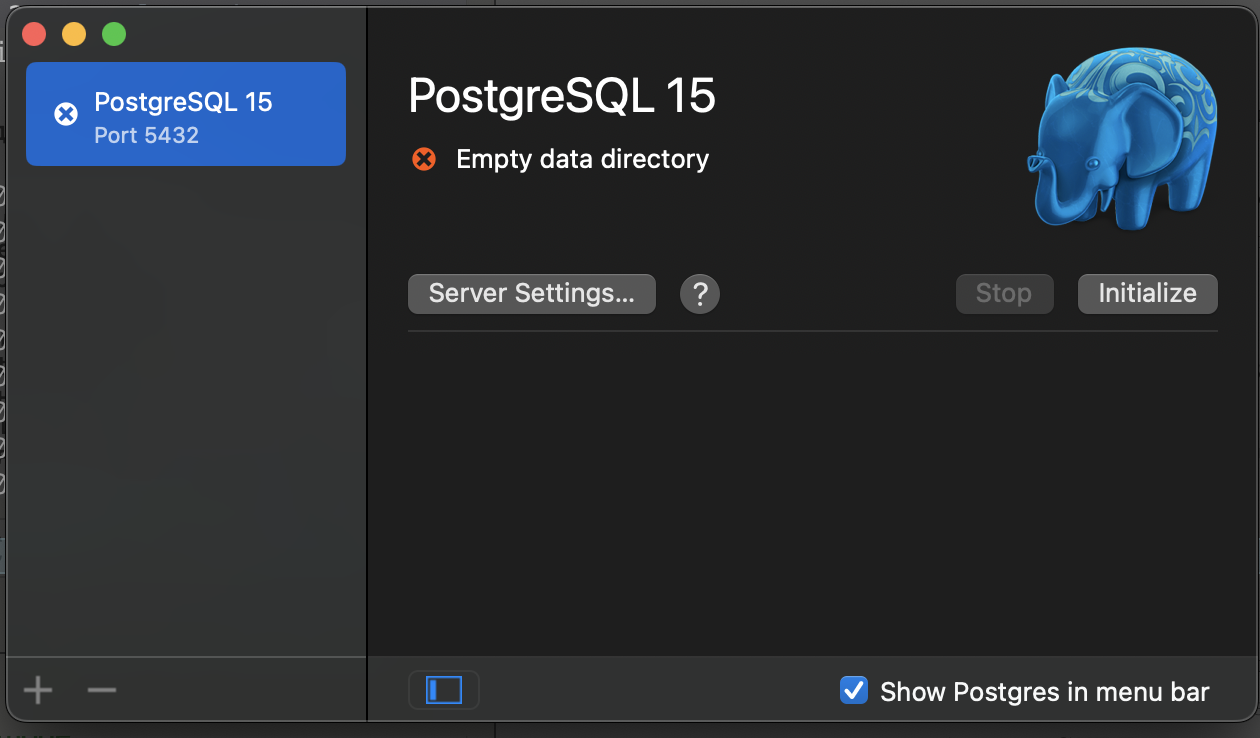
\includegraphics[scale=0.5]{figures/postgresapp.png}
	\caption{Окно приложения Postgres для MacOS X}\label{fig:postgresapp}
\end{figure}

Нажимаем кнопку \emph{Initialize} и запускаем сервер (\pic{fig:postgresapp_run_server}). Убедиться в том, что сервер запущен можно с помощью утилиты \verb|pg_ctl|
\begin{lstlisting}[
style = bash,
numbers = none
]
$ pg_ctl -D ~/Library/Application\ Support/Postgres/var-15 status
pg_ctl: server is running (PID: 48717)
/Applications/Postgres.app/Contents/Versions/15/bin/postgres "-D" "/Users/leor.finkelberg/Library/Application Support/Postgres/var-15" "-p" "5432" 
\end{lstlisting}

И так
\begin{lstlisting}[
style = bash,
numbers = none
]
$ ps aux | grep -inE postgres
...
581:leor.finkelberg  48717   0,0  0,2 34344392  15460   ??  Ss    1:42     0:00.08 /Applications/Postgres.app/Contents/Versions/15/bin/postgres -D /Users/leor.finkelberg/Library/Application Support/Postgres/var-15 -p 5432
...
\end{lstlisting}

\begin{figure}[h]
	\centering
	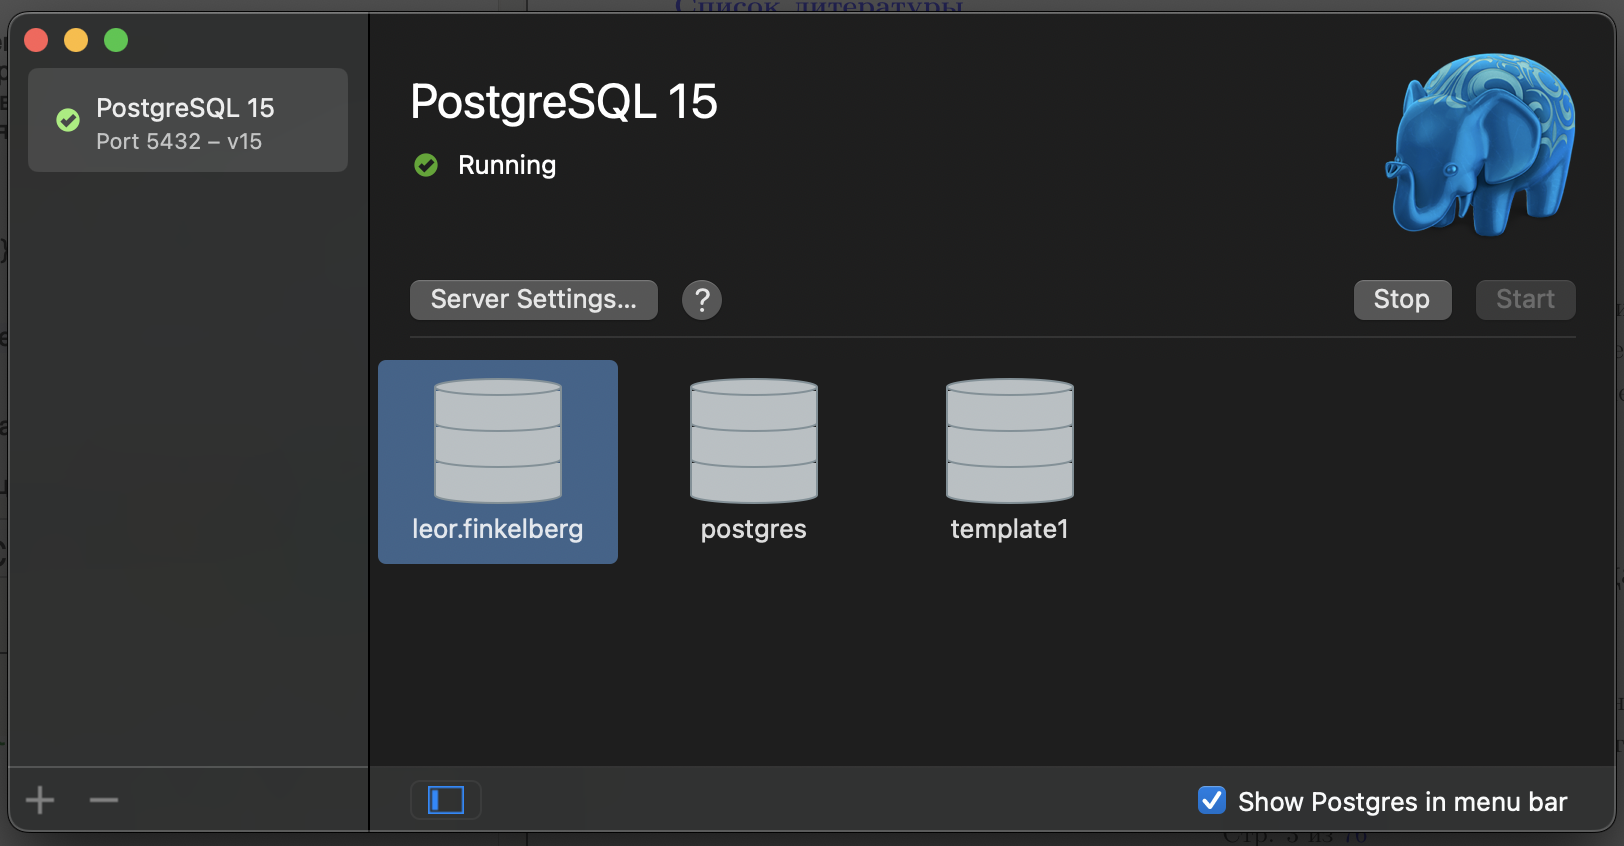
\includegraphics[scale=0.5]{figures/postgresapp_run_server.png}
	\caption{Запуск серверва PostgreSQL на MacOS X}\label{fig:postgresapp_run_server}
\end{figure}

\section{Учебные наборы данных}

Очень приличных объемов базу данных можно скачать здесь \url{https://drive.google.com/drive/folders/13F7M80Kf_somnjb-mTYAnh1hW1Y_g4kJ}

Например можно скачать sql-файл создания базы данных
\begin{lstlisting}[
style = bash,
numbers = none
]
$ unzip postgres_air.sql.zip
# запускаем в фоне
$ psql -f postgres_air.sql > psql.log 2>&1 &
# следим за ходом выполнения 
$ tail -f psql.log
\end{lstlisting}

Если создание базы данных прошло успешно, то потом нужно добавить путь к схеме базы данных
\begin{lstlisting}[
style = sql,
numbers = none
]
SET search_path TO postgres_air;
\end{lstlisting}

Проверить, что все таблицы схемы видны можно сделать так
\begin{lstlisting}[
numbers = none
]
# \dt+
\end{lstlisting}

При работе с этой базой данных полезно сразу создать кое-какие индексы
\begin{lstlisting}[
style = sql,
numbers = none
]
CREATE INDEX flight_departure_airport ON flight(departure_airport);
CREATE INDEX flight_scheduled_departure ON flight(scheduled_departure);
CREATE INDEX flight_update_ts ON flight(update_ts);
CREATE INDEX booking_leg_booking_id ON booking_leg(booking_id);
CREATE INDEX booking_leg_update_ts ON booking_leg(update_ts);
CREATE INDEX account_last_name ON account(last_name);
\end{lstlisting}

Чтобы получить результаты запросов, PostgreSQL выполняет следующие шаги \cite[\strbook{31}]{dombrovskaya:postgresql-2022}:
\begin{itemize}
	\item компилирует и преобразует инструкцию SQL в выражение, состоящее из логических операций высокого уровня, называемое логический план,
	
	\item оптимизирует логический план и превращает его в план выполнения,
	
	\item выполняет (интерпретирует) план и возвращает результаты.
\end{itemize}

\remark{
Разные серверы баз данных могут интерпретировать один и тот же запрос по-разному
}

Для оценки эффективности запроса оптимизатор использует внутренние показатели, основанные на объеме вычислительных ресурсов, необходимых для выполнения запроса или отдельной физической операции в рамках плана. Наиболее важными ресурсами являются те, что влияют на время выполнения, а именно циклы процессора и количество операций ввода-вывода (чтение и запись дисковых блоков).

Другие ресурсы, такие как память или дисковое пространство, тоже косвенно влияют на время выполнения; например, количество доступной памяти будет влиять на соотношение циклов процессора и количество операций ввода-вывода.

Эти два основных показателя, \emph{циклы процессора} и \emph{количество операций ввода-вывода}, напрямую не сопоставимы. Однако для сравнения планов выполнения запросов оптимизатор объединяет их в одну функцию стоимости: чем ниже стоимость, тем лучше план.

Любой файл, используемый для объектов базы данных, делится на блоки одинаковой длины: по умолчанию PostgreSQL использует блоки по 8192 байта каждый. \emph{Блок} -- это единица, которая передается между жестким диском и оперативной памятью, а количество операций ввода-вывода, необходимое для выполнения любого доступа к данным, равно количеству блоков, которые читаются и записываются.

Строка может быть вставлена в любой блок, в котором достаточно свободного места, без специального упорядочивания.

Все реляционные базы данных, влкючая PostgreSQL, позволяют создавать дополнительные, избыточные структуры, значительно ускоряя доступ к данным по сравнению с простым последовательным чтением.

Эти дополнительные структуры называются \emph{индексами}. Во-первых, индекс -- <<избыточные>> объекты базы данных; они не хранят никакой дополнительной информации, которую нельзя найти в исходной таблице. Во-вторых, индексы предоставляют дополнительные пути доступа к данным; они позволяют определить, какие значения храняться в строках таблицы, без необходимости чтения самой таблицы -- так работает доступ на основе индексов.

Если условие (или условия) фильтрации поддерживаются индексом в таблице, индекс можно использовать для доступа к данным из этой таблицы. Алгоритм извлекает список указателей на блоки, содержащие строки со значениями, удовлетворяющими условию фильтрации, и только эти блоки читаются из таблицы.

Основная структура данных таблицы -- это куча, то есть строки хранятся неупорядоченно. Есть две отдельные \emph{физические операции}, используемые PostgreSQL для получения \emph{строк с помощью индексов}:
\begin{itemize}
	\item \emph{индексное сканирование} (\verb|index scan|); при индексном сканировании движок базы данных считывает одну за другой все записи индекса, которые удовлетворяют условию фильтрации, и в этом же порядке извлекает блоки.
	
	\item \emph{сканирование по битовой карте} (\verb|bitmap heap scan|): поскольку базовая таблица представляет собой кучу, несколько записей индекса могут указывать на один и тот же блок; чтобы избежать многократного чтения одного и того же блока, в PostgreSQL реализована операция сканирования по битовой карте, которая создает битовую карту блоков, содержающих необходимые строки. Потом все строки в этих блоках фильтруются.
\end{itemize}

Стоимостная модель этого алгоритма намного сложнее. Неформально ее можно описать так: при малых значениях селективности, скорее всего, все строки, удовлетворяющие условиям фильтрации, будут располагаться в разных блоках, и, следовательно, стоимость бдует пропорциональна количеству возрващаемых строк. Для больших  значений селективности количество обрабатываемых блоков приближается к общему количество блоков. В последнем случае стоимость становится выше, чем стоимость полного сканирования, поскольку для доступа к индексу необходимы ресурсы \cite[\strbook{43}]{dombrovskaya:postgresql-2022}.

Если сканируется только индекс, то для малых значений селективности стоимость примерно пропорциональна количеству возвращаемых строк. При больших значениях селективности алгоритм выполняет (почти) полный просмотр индекса. Стоимость просмотра индекска обычно ниже, чем стоимость полного просмотра таблицы, потому что \emph{индекс содержит меньше данных}.

\section{Индексные структуры}

Для \emph{меньших значений селективности} предпочтительнее доступ на основе \emph{индексов}, а \emph{полное сканирование} лучше подходит для \emph{больших значений селективности} \cite[\strbook{44}]{dombrovskaya:postgresql-2022}.

\remark{
	Индексы эффективны, когда подмножество строк таблицы составляет небольшую долю от общего числа (то есть при низких значениях селективности)
}

Структура данных называется индексом, если:
\begin{itemize}
	\item это избыточная структура данных: избыточность означает, что индекс можно удалить без потери данных и восстановить по информации, хранящейся где-то еще,
	
	\item она невидима для приложения: невидимость означает, что приложение не может узнать о наличии индекса или о его отсутсвии. Иначе говоря, любой запрос дает те же результаты как с индексом, так и без него,
	
	\item она предназначена для ускорения выбора данных по определенным критериям: индекс создается в надежде, что это улучшит производительность конкретного запроса или нескольких запросов.
\end{itemize}

Улучщение производительности не происходит бесплатно. Поскольку индекс избыточен, он должен обновляться при обновлении данных таблицы. Это приводит к накладным расходам для операции обновления, которыми иногда нельзя пренебречь. В частности, индексы PostgreSQL могут оказывать большое влияние на операцию очистки (\verb|VACUUM|). Однако эти расходы как правило переоценивают. Современные высокопроизводительные СУБД используют алгоритмы, которые снижают стоимость обновления индексов, поэтому несколько индексов в таблице -- обычное дело.

Хотя индексные структуры могут значительно различаться для разных типов индексов, ускорение всегда достигается за счет \emph{быстрой проверки некоторых условий фильтрации}, указанных в запросе. Такие условия фильтрации устанавливают определенные ограничения на атрибуты таблицы.

Ни один алгоритм поиска не может найти индексный ключ среди $ N $ различных ключей быстрее, чем за время $ \log N $. Такая производительность достигается с помощью двоичноо поиска по упорядоченному списку или с помощью бинарного дерева. Однако стоимость обновлений (например, вставки новых ключей) может быть очень высока как для упорядоченных списков, так и для двоичных деревьев: вставка одной записи может привести к полной реструктуризации. Это делает обе структуры непригодными для хранения.

Напротив, \emph{B-деревья} можно изменять без значительных накладных расходов. Когда вы вставляете запись, \emph{реструктуризация ограничена одним блоком}. Даже в худшем случае количество измененных блоков не будет превышать глубины дерева \cite[\strbook{49}]{dombrovskaya:postgresql-2022}.

Если каждый блок содержит $ f $ указателей, то количество блоков на каждом уровне в $ f $ раз больше, чем в предыдущем. Следовательно, глубина дерева, содержащего $ N $ записей, равна $ \log_f N = \dfrac{\log N}{\log f} $. Эта формула дает количество обращений к диску, необходимое для поиска по одному ключу. Размер блока в PostgreSQL составляет 8 Кбайт. В такой блок помещается десятки индексных записей. следовательно, индекс с 6-7 уровнями может вместить миллиарды записей.

\section{Алгоритмы соединения}

Для больших таблиц более эффективны алгоритмы соединения хешированием и сортировки слиянием.

\subsection{Соединение хешированием}

Результат естественного соединения состоит из пар строк из таблиц R и S, которые имеют равные значения атрибутов, по которым выполняется соединение. Идея алгоритма соединения хешированием проста: если значения равны, то равны и хеш-значения.

Базовая версися алгоритма соединения хешированием включает две фазы:
\begin{itemize}
	\item на этапе построения хеш-таблицы все кортежи (строки) левой таблицы R сохраняются в корзинах согласно значениям хеш--функции,
	
	\item на этапе проверки каждая строка правой таблицы S направляется в соответствующую ей корзину. Если подходящие строки таблицы R находятся в этой корзине, порождаются выходные строки.
\end{itemize}

Алгоритм на основе хеширования значительно лучше вложенных циклов подходит для больших таблиц и большого количества различных значений атрибута соединения.

Базовый алгоритм соединения хешированием работает, если все корзины, созданные на этапе построения хеш-таблицы, помещаются в оперативную память. 

Другой вариант, называемый \emph{гибридным соединением хешированием}, соединяет таблицы, которые не могут поместиться в оперативной памяти. Гибридное соединение хешированием разделяет обе таблицы так, чтобы отдельные разделы помещались в память, а затем выполняет базовый алгоритм для каждой пары соотвествующих разделов. Стоимость гибридного соединения хешированием выше, потому что разделы временно храняться на жестком диске и обе таблицы сканируются дважды.

\subsection{Сортировка слиянием}

На первом этапе алгоритма обе входные таблицы сортируются в порядке возрастания по атрибутам соединения.

После того как таблицы правильно упорядочены, на этапе слияния обе таблицы сканируются один раз и для каждого значения атрибута соединения вычисляется декартово произведение строк, содержащих это значение.

Алгоритм сортировки слиянием особенно эффективен, если одна или обе входные таблицы уже отсортированы.

\section{Чтение планов выполнения}

Рассмотрим запрос
\begin{lstlisting}[
style = sql,
numbers = none
]
SELECT
  f.flight_no, -- атрибут группировки
  f.actual_departure,  -- атрибут группировки
  count(passenger_id) passengers
FROM
  flight f
    JOIN booking_leg bl ON bl.flight_id = f.flight_id
    JOIN passenger p ON p.booking_id = bl.booking_id
WHERE
  f.departure_airport = 'JFK'
  AND f.arrival_airport = 'ORD'
  AND f.actual_departure BETWEEN '2020-08-14' AND '2020-08-15'
GROUP BY f.flight_no, f.actual_departure; -- атрибуты группировки должна быть в списке выборки
\end{lstlisting}

Чтобы получить план выполнения запроса, используется команда \verb|EXPLAIN query|.

План содержит:
\begin{itemize}
	\item оценки стоимости,
	
	\item ожиадемое количество выходных строк,
	
	\item ожидаемый средний размер (<<ширину>>) строк.
\end{itemize}

Значения стоимости включают в себя совокупную стоимость:
\begin{itemize}
	\item первая показывает стоимость, необходимую для создания первой строки вывода,
	
	\item  в то время как вторая оценивает \emph{полную стоимость получения всего результата}.
\end{itemize}

Важно подчеркнуть, что все эти цифры являются приблизительными. План выполнения представляется в виде дерева физических операций. В этом дереве узлы представляют операции, а стрелки указывают на операнды.




\section{Замечания по использованию различных баз данных для различных проектов}

Небольшому стартапу лучше выбрать одну из реляционных баз данных, например, MySQL или PostgreSQL -- они подходят для широкого круга задач. Быстрорастущим компаниям есть смысл использовать сразу две-три СУБД. Например, MySQL или PostgreSQL для длительного хранения данных, а Redis -- для быстрой обработки запросов.

Проще и дешевле масштабировать облачные базы данных -- для проектов с непредсказуемой нагрузкой лучше всего подходят PostgreSQL или MongoDB в конфигурации, предназначенной для быстрого выделения ресурсов. В случае резкого роста трафика компания получает дополнительные мощности облачной СУБД автоматически или по запросу. При этом оплачиваются только фактически потраченные ресурсы.

Если информации для анализа очень много и требуется чтобы машинный алгоритм мог сделать выводы на их основе, необходимо быстро извлекать данные по заданным критериям. С этой задачей не справятся реляционные базы данных MySQL и PostgreSQL -- они долго обрабатывают большие массивы информации. Здесь нужна специальная аналитическая база данных, например, ClickHouse. Она быстро выполняет аналитические запросы.

Некоторые сервисы должны быстро обрабатывать запросы пользователей, в том числе в режиме реального времени -- для проведения транзакций, аналитики в реальном времени, счетчиков, аутентификации и других операциях, предполагающих быстрый ответ базы данных. Для таких ситуаций подойдет Redis -- нереляционная высокопроизводительная СУБД. Redis хранит данные в оперативной памяти, за счет этого отвечает на запросы в десятки раз быстрее, чем MySQL или PostgreSQL. Redis можно использовать и как самостоятельную СУБД, и как дополнительную СУБД в тех случаях, когда число запросов резко растет и нужно быстро их обработать.

Иногда бизнесу требуется решать узко специализированные задачи. Например, шифровать пароли, составлять рейтинги, анализировать маршруты транспорта или следить за передвижением курьеров в реальном времени. Нужна база данных, позволяющая подключать расширения или использовать команды для решения нестандартных задач. 

Для PostgreSQL и Postgres Pro разработано большое количество дополнительных расширений. Например, расширение для криптографии шифрует личные данные для безопасной передачи по сети. В случае кражи злоумышленники получают только обезличенную информацию. А расширение PostGIS подходит для картографических сервисов, например, для поиска по географическим данным.

В Redis есть наборы специальных команд и операторов, позволяющих использовать базу данных для решения узких задач в режиме реального времени. Например, составления рейтингов игроков в играх, аналитики контента, управления геоданными, в том числе отслеживания местоположения транспорта.

Итак:
\begin{itemize}
	\item У стартапа может смениться бизнес-модель. Поэтому лучше выбрать СУБД, подходящую для решения широкого круга задач, или заложить сразу две-три базы данных,
	
	\item В бизнесе, где нагрузка на инфраструктуру зависит от сезона, важно быстро масштабировать базу данных -- это удобно делать в облаке,
	
	\item Хранить информацию в неизменном виде позволяют реляционные базы данных, например, MySQL или PostgreSQL,
	
	\item Для работы с большими данными подойдет ClickHouse -- база данных, позволяющая быстро выполнять аналитические запросы,
	
	\item Быстро отвечать на запросы пользователей позволяет Redis -- нереляционная высокопроизводительная СУБД, она хранит данные в оперативной памяти.
\end{itemize}

\section{Ответвления от PostgreSQL}

От PostgreSQL существует более 20 ответвлений. На протяжении многих лет различные группы создавали ответвления и затем включали результаты своей работы в PostgreSQL:
\begin{itemize}
	\item HadoopDB -- гибрид PostgreSQL с технологиями MapReduce, ориентированный на аналитику,
	
	\item Greenplum -- реляционная СУБД, имеющая массово-параллельную архитектуру без разделения ресурсов. Или еще можно сказать, что Greeplumn представляет собой кластер над экземплярами PostgreSQL без разделения ресурсов с массово параллельной обработкой (MPP). Применяется для создания хранилищ данных и аналитики,
	
	\item Vertica -- столбцовая СУБД ориентированная на аналитику данных. Терминальный клиент для Python можно изучить на странице проекта \url{https://github.com/vertica/vertica-python},
	
	\item Amazon Redshift -- популярное хранилище данных на базе PostgreSQL 8.0.2. Предназначено в основном для OLAP-приложений. 
\end{itemize}

С различными СУБД (реляционными, нереляционными, аналитическими, графовыми, документарными и пр.) удобно работать с помощью кроссплатформенного менеджера баз данных \texttt{DBeaver} \url{https://dbeaver.io/download/}.

\subsection{Базовые сведения о \texttt{Greenplum}}

\texttt{Greenplum} -- реляционная СУБД с массово-параллельной архитектурой без разделения ресурсов, ориентированная на OLAP-приложения. Другими словами, основная задача \texttt{Greenplum} работа с аналитической нагрузкой. \texttt{PostgreSQL} это все-таки классическая реляционная СУБД ориентированная главным образом на OLTP-приложения, хотя с помощью этой СУБД можно строить и отностительно простые OLAP-приложения. Индексы, которые активно используются в \texttt{PostgreSQL}, полезны для OLTP-задач, но бесполезны в OLAP-задачах. Индексы эффективны, когда подмножество строк таблицы составляет небольшую долю от общего числа. В аналитических же задачах приходится работать с широкими длинными таблицами, т.е. с таблицами, у которых несколько сотен столбцов и очень много строк, порядка нескольких сотен тысяч или даже нескольких миллионов строк.

Профиль аналитической нагрузки:
\begin{itemize}
	\item <<Широкие>> таблицы (сотни столбцов, много строк),
	
	\item Работа большими пакетами данных (чтение, вставка),
	
	\item При чтении обрабатывается много строк, но мало столбцов (1 - 10\%),
	
	\item Обновления и удаления редки,
	
	\item Мало параллельных запросов в системе,
	
	\item Допустимы задержки при получении результата.
\end{itemize}

Цель: максимизация пропускной способности запроса.


Кластеры бывают гомогенные (все ноды кластера одинаковые) и с ролями (часть нод выполняют одну роль, часть другую, часть третью). Ноды могут представлять собой либо просто экземпляры СУБД, либо отказоустойчивые группы.

Так вот \texttt{Greenplum} это кластер на ролях с отказоустойчивыми группами. Здесь отказоустойчивая группа это пара <<Мастер-Резерв>> (Dispatch). Она управляет другими группами, которые хранят данные (Execute). В эти группы входят сегмент и зеркало.

\texttt{Greenplum} остается транзакционной системой в отличие от прочих аналитических решений.

\remark{
\texttt{Greenplum} \emph{не нужно} использовать в OLTP-приложениях, т.е. в приложениях, в которых речь идет о \emph{транзакционной нагрузке}
}

\texttt{Greenplum} лучше всего справляется с:
\begin{itemize}
	\item Сложные запросы, обрабатывающие большие объемы (в том числе сложные аналитические функции и т.д.),
	
	\item {ETL}/{ELT},
	
	\item Работа с индексами,
	
	\item Data Science,
	
	\item Аналитические функции на PL,
	
	\item Ad-hoc аналитика (когда мы не знаем какой запрос напишет пользователь).
\end{itemize}


\section{Хранилища данных}

Хранилище данных (Data Warehouse) -- предметно-ориентированная информационная база данных, специально разработанная и предназначенная для подготовки отчетов и бизнес-анализа с целью поддержки принятия решений в организации. Строится на базе систем управления базами данных и систем поддержки принятия решений. Данные, поступающие в хранилища, как правило, доступны только для чтения.

Существует два варианта \emph{обновления} данных в хранилище:
\begin{itemize}
	\item \emph{полное} обновление данных в хранилище. Сначала старые данные удаляются, потом происходит загрузка новых данных. Процесс выполняется с определенной периодичностью, при этом актуальность данных может несколько отставать от OLTP-системы,
	
	\item \emph{инкрементальное} обновление -- обновляются только те данные, которые изменились в OLTP-системе.
\end{itemize}

Принципы организации хранилища:
\begin{itemize}
	\item \emph{Проблемно-предметная ориентация}: данные объединяются в категории и хранятся в соответствии с областями, которые они описывают, а не с приложениями, которые они используют,
	
	\item \emph{Интегрированность}: данные объединены так, чтобы они удовлетворяли всем требованиям предприятия в целом, а не единственной функции бизнеса,
	
	\item \emph{Некорректируемость}: данные в хранилище не создаются; то есть данные поступают из внешних источников, не корректируются и не удаляются,
	
	\item \emph{Зависимость от времени}: данные в хранилище точны и корректны только в том случае, когда они привязаны к некоторому промежутку или моменту времени.
\end{itemize}

Существует два архитектурных направления:
\begin{itemize}
	\item {нормализованные хранилища данных},
	
	\item  {хранилища данных с измерениями}.
\end{itemize}

В нормализованных хранилищах, данные находятся в предметно-ориентированных таблицах третьей нормальной формы. Нормализованные хранилища характеризуются как простые в создании и управлении, недостатки нормализованных таблиц -- большое количество таблиц как атрибут нормализации, в следствие чего для получения какой-либо информации нужно делать выборку из многих таблиц одновременно, что приводит к снижению производительности системы. Для решения этой проблемы используются денормализованные таблицы -- витрины данных, на основе которых уже выводятся отчетные формы. При очень больших объемах данных могут использоваться несколько уровней витрин/хранилищ.

Хранилища с измерениями, как правило, используют схему <<звезда>> или <<снежинка>>. При этом в центре <<звезды>> находятся данные (таблица фактов), а измерения образуют лучи звезды. Различные таблицы фактов совместно используют таблицы измерений, что значительно облегчает операции объединения данных из нескольких предметных таблиц фактов. Основным недостатком является более сложные процедуры подготовки и загрузки данных, а также управление и изменение измерений данных.

\section{Основные ошибки при работе с \texttt{PostgreSQL}}

Отличный доклад Алексея Лесовского \url{https://www.youtube.com/watch?v=HjLnY0aPQZo&list=PL2SBCjiIRNXBIARbUE-BprXkH-HhZ2xr4&index=7}.

Чаще всего при работе с PostgreSQL не хватает дискового пространства или дисковой производительности.

Есть OLTP-нагрузка, которая характеризуется быстрыми, легкими, короткими запросами, и OLAP-нагрузка, характеризующаяся медленными, долгими, тяжелыми аналитическими запросами, которые вычитывают большие объемы данных.

Практика показывает, что нужно разносить OLTP и OLAP части, хотя бы потому, что OLAP-запросы блокируют OLTP-запросы.

PostgreSQL поддерживает \emph{потоковую} и \emph{логическую} репликацию. В отличие от потоковой репликации, при которой двоичные данные копируются побитово, механизм логической репликации преобразует WAL-файлы в набор логических изменений. Логическая репликация позволяет скопировать часть данных, тогда как в случае потоковой репликации ведомый узел является точной копией ведущего. 

Организовать независимую работу OLAP и OLTP запросов можно с помощью \emph{потоковой репликации} (поддерживаются синхронная, асинхронная и каскадная репликации). В каскадном режиме ведомый узел является ведущим для другой реплики. Это позволяет горизонтально масштабировать PostgreSQL на операциях чтения.

Можно использовать механизм \emph{логической репликации}\footnote{Еще называют механизмом логических публикаций и подписок}. Когда есть несколько независимых PostgreSQL-серверов со своими базами. Эти базы можно подключать в соседние базы. Все изменения источников будут реплицироваться на базу назначения и там будут видны.

Другой подход, \emph{декларативное партиционирование} и механизм внешних таблиц. Пусть есть несколь PostgreSQL-серверов, которые хранят данные за какие-то диапазоны. Сводную базу данных, имеющую доступ к партициям хранят на мастер-сервере.

И, наконец, эти схемы можно комбинировать.

Начать имеет смысл с разнесения нагрузки. В мастер идет запись, а с реплик выполняется чтение. Для выполнения сложных аналитических запросов нужна отдельная реплика.

Еще важно помнить, что базы данных это все-таки не хранилище, они больше ориентированны на конкурентный доступ. Не нужно строить индексы на все случаи жизни. Индексы снижают время обновления и в случае аварии время восстановления. Если строится индекс, то должна быть железная уверенность в том, что он там нужен.


Основные рекомендации:
\begin{itemize}	
	\item Базу данных следует размещать на SSD. Это надежное, устойчивое решение,
	
	\item Нельзя писать в базу данных все подряд,
	
	\item Важно проводить партиционирование (секционирование) данных,
	
	\item Очень важно организовать мониторинг\footnote{Можно следить за статусом клиентов, ошибками (появились ошибки, есть повод заглянуть в log), качественными/количественными показателями запросов (нет ли медленных запросов, например)}; нельзя использовать конфигурационные файлы с настройками по умолчанию, важно уметь конфигурировать PostgreSQL,
	
	\item Надо стараться разнести потоки чтения и записи, т.е. лучше не читать и не писать в одно и то же место; PostgreSQL очень хорошо масштабируется,
	
	\item Очень важно контролировать ничего не делающие транзакции, они снижают производительность и убивают базу,
	
	
\end{itemize}
 

\section{Файл подкачки}

Подкачка страниц представляет собой механизм виртуальной памяти, перемещающий неиспользуемые (неактивные) фрагменты памяти в другое хранилище (жесткий диск или какое-либо другое место), тем самым освобождая место в оперативной памяти для загрузки активных данных. В качестве хранилища могут выступать раздел подкачки или файл подкачки (swap-файл). Раздел подкачки обычно создается в момент установки операционной системы, а файл подкачки можно создать в любой момент, главное чтобы было место.

Пространство подкачки главным образом используется для расширения виртуальной памяти за пределы установленной оперативной памяти (RAM).

Ресурс твердотельных накопителей (SSD) напрямую зависит от числа циклов записи/перезаписи, поэтому не рекомендуется использовать swap на SSD.

\section{Первичные и внешние ключи}

\emph{Ограничение внешнего ключа} указывает, что значения столбца (или группы столбцов) должны соответствовать значениям в некоторой строке другой таблицы. Или другими словами ограничение внешнего ключа обеспечивает \emph{ссылочную целостность} связанных таблиц.

\emph{Ограничение первичного ключа} означает, что образующий его столбец или группа столбцов может быть уникальным идентификатором строк в таблице. Или другими словами обеспечивает \emph{сущностную целостность}.

\begin{lstlisting}[
style = sql,
numbers = none	
]
CREATE TABLE products (
  product_no integer PRIMARY KEY, -- первичный ключ уровня столбца
  name text,
  price numeric
);

CREATE TABLE orders (
  order_id integer PRIMARY KEY, -- первичный ключ уровня столбца
  shipping_address text,
  ...
);

CREATE TABLE order_items (
  product_no integer REFERENCES products ON DELETE RESTRICT, -- внешний ключ уровня столбца (ограничивающее удаление)
  order_id integer REFERENCES orders ON DELETE CASCADE, -- внешний ключ уровня столбца (каскадное удаление)
  quantity integer,
  PRIMARY KEY (product_no, order_id) -- составной первичный ключ уровня таблицы
);
\end{lstlisting}

Ограничивающие и каскадные удаления — два наиболее распространённых варианта. \texttt{RESTRICT} предотвращает удаление связанной строки. \texttt{NO ACTION} означает, что если зависимые строки продолжают существовать при проверке ограничения, возникает ошибка (это поведение по умолчанию). Главным отличием этих двух вариантов является то, что \texttt{NO ACTION} позволяет отложить проверку в процессе транзакции, а \texttt{RESTRICT} -- нет.

\texttt{CASCADE} указывает, что при удалении связанных строк зависимые от них будут так же автоматически удалены. Есть ещё два варианта: \texttt{SET NULL} и \texttt{SET DEFAULT}. При удалении связанных строк они назначают зависимым столбцам в подчинённой таблице значения \texttt{NULL} или значения по умолчанию, соответственно. Если в качестве действия задано \texttt{SET DEFAULT}, но значение по умолчанию не удовлетворяет ограничению внешнего ключа, операция закончится ошибкой.

\section{Буферный кеш в \texttt{PostgreSQL}}

Размер кеша устанавливается параметром \verb|shared_buffers|. Значение по умолчанию смехотворное -- 128 Мб. Это один из параметров, которые имеет смысл увеличить сразу же после установки PostgreSQL.

\begin{lstlisting}[
style = sql,
numbers = none
]
SELECT setting, unit
FROM pg_settings
WHERE name = 'shared_buffers';
\end{lstlisting}

\begin{lstlisting}[
style = bash,
numbers = none
]
+---------+------+
| setting | unit |
+---------+------+
| 16384   | 8kB  |
+---------+------+
\end{lstlisting}

Надо иметь в виду, что изменение параметра требует перезапуска сервера, поскольку вся необходимая под кеш память выделяется при старте сервера.

Оптимальное значение буферного кеша зависит данных, приложения, нагрузки и т.п. Стандартная рекомендация -- взять в качестве первого приближения 1/4 оперативной памяти, а дальше по ситуации.

Исключение из общего правила представляют временные таблицы. Поскольку временные данные видны только одному процессу, им нечего делать в общем буферном кеше. Более того, временные данные существуют только в рамках одного сеанса, так что их не нужно защищать от сбоя.

Для временных данных используется кеш в локальной памяти того процесса, который владеет таблицей. Поскольку такие данные доступны только одному процессу, их не требуется защищать блокировками. В локальном кеше используется обычный алгоритм вытеснения. 

В отличие от общего буферного кеша, память под локальный кеш выделяется по мере необходимости, ведь временные таблицы используются далеко не во всех сеансах. Максимальный объем памяти для временных таблиц одного сеанса ограничен параметром \verb|temp_buffers|.

Для справки перезапустить сервер на Windows, используя командную оболочку \texttt{bash}, можно с помощью утилиты \verb|pg_ctl|\footnote{Еще перезагрузить кластер после внесения изменений в файл \texttt{pg\_hba.conf} или \texttt{postgresql.conf} можно с помощью функции \texttt{pg\_reload\_conf()}} так
\begin{lstlisting}[
style = bash,
numbers = none
]
pg_ctl restart -D '/c/Program Files/PostgreSQL/11/data'
\end{lstlisting}
или так, если использовать \texttt{cmd.exe}
\begin{lstlisting}[
style = bash,
numbers = none
]
pg_ctl restart -D "C:\Program Files\PostgreSQL\11\data"
\end{lstlisting}

А посмотреть статус можно так
\begin{lstlisting}[
style = bash,
numbers = none
]
pg_ctl status -D "C:\Program Files\PostgreSQL\11\data"
\end{lstlisting}

Для справки все изменения (например, изменение номера порта), вносимые в файл \texttt{postgresql.conf} требуют перезапуска сервера, т.е. \verb|pg_ctl restart -D "C:\Prog...\data"|.

Помимо \texttt{set\_config}, PostgreSQL предоставляет для изменения конфигурационных параметров команду \texttt{ALTER SYSTEM} со следующим синтаксисом
\begin{lstlisting}[
style = sql,
numbers = none
]
ALTER SYSTEM SET configuration_parameter { TO | = } { value | 'value' | DEFAULT }
ALTER SYSTEM RESET configuration_parameter
ALTER SYSTEM RESET ALL
\end{lstlisting}

Иногда для вступления значения в силу требуется перезагрузка системы или перезапуск
\begin{lstlisting}[
style = sql,
numbers = none
]
$ SHOW work_mem; -- 4MB
$ ALTER SYSTEM SET work_mem TO '8MB';
$ SELECT pg_reload_config();
$ SHOW work_mem; -- 8MB
\end{lstlisting}

Получить список параметров, значения которым присвоены в файле \texttt{postgresql.conf}, а не по умолчанию можно так
\begin{lstlisting}[
style = sql,
numbers = none
]
SELECT name, current_setting(name), source
FROM pg_settings
WHERE source IN ('configuration file');
\end{lstlisting}

Получить размер базы данных можно с помощью специальных функций
\begin{lstlisting}[
style = sql,
numbers = none
]
SELECT datname, pg_size_pretty(pg_database_size(datname)) AS size
FROM pg_database;
\end{lstlisting}
выведет
\begin{lstlisting}[
style = bash,
numbers = none
]
+-----------+---------+
|  datname  |  size   |
+-----------+---------+
| postgres  | 8393 kB |
| demo      | 304 MB  |
| template1 | 7769 kB |
+-----------+---------+
\end{lstlisting}

Функция \texttt{pg\_total\_relation\_size()} возвращает размер таблицы со всеми индексами и TOAST-таблицами. Если интересует только размер самой таблицы, то следует воспользоваться функцией \texttt{pg\_relation\_size()}. Эта информация поможет следить за ростом таблицы и табличных пространств
\begin{lstlisting}[
style = sql,
numbers = none
]
SELECT pg_size_pretty(pg_total_relation_size('table'));
\end{lstlisting}

Наконец, размер индекса также вернет функция \texttt{pg\_relation\_size()}
\begin{lstlisting}[
style = sql,
numbers = none
]
SELECT indexrelid::regclass, pg_size_pretty(pg_relation_size(indexrelid::regclass))
FROM pg_index
LIMIT 2;
\end{lstlisting}

\section{План выполнения запроса и команда \texttt{EXPLAIN}}

У команды \texttt{EXPLAIN} есть несколько опций; при наличии опции \texttt{ANALYZE} команда выполняется и возвращает фактическое время и количество строк.

Для поддержания статистики базы данных в актуальном состоянии важно, чтобы работал процесс автоочистки.

Разумеется, если статистика неправильная, то ожидать хороших планов выполнения не приходится. После \emph{массовой загрузки данных} в базу рекомендуется выполнить команду \texttt{ANALYZE} для обновления статистики. 

Рассмотрим пример плана выполнения запроса
\begin{lstlisting}[
style = bash,
numbers = none
]
--------------------------------------------------------------------
Seq Scan on <table_name> (cost=0.00..1834.00 rows=100000 width=37)
\end{lstlisting}

Стоимость запроса (cost) -- это оценка затрат на его выполнение. В этом примере \texttt{0.00} -- стоимость выборки \emph{первой строки}, \texttt{1834.00} -- стоимость выборки \emph{всех} строк, вычисляемая по формуле \texttt{(relpages*seq\_page\_cost) + (reltuples*cpu\_tuple\_cost)}. Количество страниц отношения (\texttt{relpages}) и строк отношения (\texttt{reltuples}) можно найти в таблице \texttt{pg\_class}. Величины \texttt{seq\_page\_cost} и \texttt{cpu\_tuple\_cost} -- это конфигурационные параметры планировщика. Таким образом мы получаем число 1834.

В этом простом примере последовательного просмотра вычислить стоимость не составляет труда. Но если запрос включает вычисление предикатов, группировку, сортировку и соединение, то получить оценку стоимости гораздо сложнее. Наконец, величина 37 в плане выполнения -- это средняя ширина кортежа в байтах, которую можно найти в таблице \texttt{pg\_stats}. 

Чтобы выполнить запрос и одновременно получить его стоимость, имеется команда \texttt{EXPLAIN ANALYZE}. План запроса следует читать снизу вверх, начиная строки с наибольшим отступом.

Выполнить запрос и вывести его план можно и так
\begin{lstlisting}[
style = bash,
numbers = none
]
EXPLAIN (ANALYZE, FORMAT YAML, BUFFERS) SELECT * FROM <table_name>;
\end{lstlisting}

выведет что-то похожее на
\begin{lstlisting}[
style = bash,
numbers = none
]
+--------------------------------+
|           QUERY PLAN           |
+--------------------------------+
| - Plan:                       +|
|     Node Type: "Seq Scan"     +|
|     Parallel Aware: false     +|
|     Relation Name: "test_json"+|
|     Alias: "test_json"        +|
|     Startup Cost: 0.00        +|
|     Total Cost: 1.03          +|
|     Plan Rows: 3              +|
|     Plan Width: 105           +|
|     Actual Startup Time: 0.019+|
|     Actual Total Time: 0.021  +|
|     Actual Rows: 3            +|
|     Actual Loops: 1           +|
|     Shared Hit Blocks: 1      +| <-- NB!
|     Shared Read Blocks: 0     +|
|     Shared Dirtied Blocks: 0  +|
|     Shared Written Blocks: 0  +|
|     Local Hit Blocks: 0       +|
|     Local Read Blocks: 0      +|
|     Local Dirtied Blocks: 0   +|
|     Local Written Blocks: 0   +|
|     Temp Read Blocks: 0       +|
|     Temp Written Blocks: 0    +|
|   Planning Time: 0.105        +|
|   Triggers:                   +|
|   Execution Time: 0.048        |
+--------------------------------+
\end{lstlisting}

Строка <<\texttt{Shared Hit Blocks: 1}>> (разделяемые блоки в кеше) означает, что данные читаются из памяти, а не с диска.

\subsection{Обнаружение проблем в планах выполнения запросов}

Команда \texttt{EXPLAIN} может показать, почему запрос работает медленно, особенно если выполнять ее с опциями \texttt{BUFFER} и \texttt{ANALYZE}. Вот на что следует обращать внимание, пытаясь понять, хорош план выполнения или нет:
\begin{itemize}
	\item \emph{Оценка числа строк и истинное число строк}. Это важно, потому что планировщик ориентируется на эту величину, выбирая метод выполнения запроса. Есть два случая: оценка числа строк завышена или занижена. Неправильная оценка влияет на все алгоритмы: выборки данных с диска, сортировки, соединения и т.д. Вообще говоря, завешенная оценка -- это нехорошо, но \emph{заниженная} -- гораздо хуже. С одной стороны, при выполнении соединения очень больших таблиц методом вложенных циклов время выполнения растет экспоненциально, если для простоты предположить, что стоимость этого алгоритма равно $ O(n^2) $. С другой стороны, соединение с небольшой таблицей методом хеширования замедляет выполнение запроса, но эффект оказывается не таким чудовищным, как в первом случае.
	
	\item \emph{Сортировка в памяти или на диске}. Сортировка выполняется при наличии таких фраз, как \texttt{DISTINCT}, \texttt{LIMIT}, \texttt{ORDER}, \texttt{GROUP BY}, и некоторых других. Если памяти достаточно, то сортировка производится в памяти, иначе на диске.
	
	\item \emph{Буферный кеш}. Важно обращать внимание на то, сколько данных находится в буферах и сколько из них грязных. Чтение данных из буфера значительно повышает производительность.
\end{itemize}

\remark{%
Если план выполнения длинный и сложный и трудно понять в чем <<затык>>, то можно попробывать запретить алгоритм с экспоненциальным временем работы, например \emph{соединение методом вложенных циклов}
}

Еще один очень любопытный момент связан с \emph{межстолбцовой корреляцией}. Из-за межстолбцовой корреляции возможны ошибки в оценке количества строк, поскольку PostgreSQL предполагает, что все столбцы независимы. Но на самом деле это далеко не всегда так. Пример -- страна и язык в предпочтениях клиентов. 

Чтобы избежать проблем, связанных с межстолбцовой корреляцией, следует объединять такие столбцы в один с типом \texttt{jsonb}.

В PostgreSQL 10 добавлена перекрестная статистика столбцов, так что больше менять физическую структуру таблицы не нужно. Однако необходимо уведомить планировщик о наличии таких зависимостей. Чтобы расширить статистику, выполним такую команду
\begin{lstlisting}[
style = sql,
numbers = none
]
CREATE STATISTICS stats(dependenies) ON country, language FROM client;
\end{lstlisting}


\section{Сброс пароля для \texttt{psql} и \texttt{pgAdmin4}}

Для того чтобы доступ к базам данных через терминальный клиент \texttt{psql} или через web-интерфейс \texttt{pgAdmin4} можно было выполнять без ввода пароля, нужно сделать следующее:
\begin{itemize}
	\item найти файл \texttt{pg\_hba.conf}; на ОС Windows он располагается по адресу \directory{C: > Program Files > PostgreSQL > 11 > data},
	
	\item заменить в этом файле метод \texttt{md5} (в нижней части файла) на \texttt{trust}.
\end{itemize}

После исправлений файл \texttt{pg\_hba.conf} должен выглядеть приблизительно так
\begin{lstlisting}[
title = {\sffamily pg\_hba.conf},
style = bash,
numbers = none
]
...
# TYPE  DATABASE        USER            ADDRESS                 METHOD

# IPv4 local connections:
host    all             all             127.0.0.1/32            trust
host    all             all             0.0.0.0/0               trust
# IPv6 local connections:
host    all             all             ::1/128                 trust
host    all             all             ::0/0                   trust
# Allow replication connections from localhost, by a user with the
# replication privilege.
host    replication     all             127.0.0.1/32            trust
host    replication     all             ::1/128                 trust
host    appdb           app             all                     trust

\end{lstlisting}

\section{Создание резервной копии базы данных}

Задачу резервного копирования можно запускать с выделенного backup-сервера или с сервера базы данных. В комплекте PostgreSQL есть 2 утилиты, которые позволяют делать резервные копии: \texttt{pg\_dump}, \texttt{pg\_dumpall} (сохраняют резервную копию базы данных в текстовом файле или другом виде) и \texttt{pg\_basebackup} (делает базовую резервную копию \emph{работающего} сервера PostgreSQL). Кроме того есть возможность использовать утилиты файлового копирования, такие \texttt{rsync}, \texttt{tar}, \texttt{cp} и т.п.

Утилита \texttt{pg\_dump} подходит для случаев, когда нужно сделать резервную копию таблицы, базы или схемы, а \texttt{pg\_basebackup} -- подходит для случаев, когда нужно сделать резервную копию целиком всего кластера базы данных или настроить реплику. Утилиты \texttt{rsync}, \texttt{tar}, \texttt{cp} также используются для случаев копирования всего кластера.

Примеры создания резервной копии базы данных
\begin{lstlisting}[
style = bash,
numbers = none
]
pg_dump -U postgres -d demo --format=tar -v -f $(date +%Y-%m-%d).demo.tar
pg_dump -U postgres -d demo -f $(date +%Y-%m-%d).demo.sql
\end{lstlisting}

Создать резервную копию с backup-сервера в каталог \directory{/backup} (каталог должен существовать)
\begin{lstlisting}[
style = bash,
numbers = none
]
pg_basebackup -x -h db01.example.com -U backup -D /backup

\end{lstlisting}

Копирование со сжатием в bzip2, для случаев, когда нужно использовать нестандартный алгоритм сжатия
\begin{lstlisting}[
style = bash,
numbers = none
]
pg_basebackup -x --format=tar -h db01.example.com -U backup -D - | bzip2 -9 > /backup/db01/backup-$(date +%Y-%m-%d).tar.bz2
\end{lstlisting}

Копирование со сжатием в несколько потоков (задействуем 8 ядер)
\begin{lstlisting}[
style = bash,
numbers = none
]
pg_basebackup -x --format=tar -h db01.example.com -U backup -D - | lbzip2 -n 8 -9 > /backup/db01/backup-$(date +%Y-%m-%d).tar.bz2
\end{lstlisting}

Копирование запускается на сервере базы данных. Формируемая резервная копия отправляется на удаленный сервер по ssh
\begin{lstlisting}[
style = bash,
numbers = none
]
pg_basebackup -x --format=tar -h 127.0.0.1 -U backup -D - | \
    ssh backup@backup.example.com "tar -xf - -C /backup/"
\end{lstlisting}

Восстановить данные из созданных backup-файлов можно с помощью утилиты \texttt{pg\_restore}.




\section{Логический порядок обработки инструкции \texttt{SELECT}}

Порядок обработки инструкции \texttt{SELECT} определяет, когда объекты, определенные в одном шаге, становятся доступными для предложений в последующих шагах. Например, если обработчик запросов можно привязать к таблицам или представлениям, определенным в предложении \texttt{FROM}, эти объекты и их столбцы становятся доступными для всех последующих шагов.

Общая процедура выполнения \texttt{SELECT} следущая (подробности см. в документации~\href{https://postgrespro.ru/docs/postgresql/9.5/sql-select}{\texttt{SELECT}}):

\begin{enumerate}
	\item \texttt{WITH}: выполняются все запросы в списке \texttt{WITH}; по сути они формируют временные таблицы, к которым затем можно обращаться в списке \texttt{FROM}; запрос в \texttt{WITH} выполняется только один раз, даже если он фигурирует в списке \texttt{FROM} неоднократно,
	
	\item \texttt{FROM}: вычисляются все элементы в списке \texttt{FROM} (каждый элемент в списке \texttt{FROM} представляет собой реальную или виртуальную таблицу); другими словами конструируются таблицы из списка \texttt{FROM},
	
	\item \texttt{ON}: выбираются строки, удовлетворяющие заданному условию,
	
	\item \texttt{JOIN}: выполняется объединение таблиц,
	
	\item \texttt{WHERE}: исключаются строки, не удовлетворяющие заданному условию,
	
	\item \texttt{GROUP BY}: вывод разделяется по группам строк, соответствующим одному или нескольким значениям, а затем вычисляются результаты агрегатных функций,
	
	\item \texttt{HAVING}: исключаются группы, не удовлетворяющие заданному условию,
	
	\item \texttt{SELECT},
	
	\item \texttt{DISTINCT}: исключаются \emph{повторяющиеся} строки; \texttt{SELECT DISTINCT ON} исключает строки, совпадающие по всем указанным выражениям; \texttt{SELECT ALL} (по умолчанию) возвращает все строки результата, включая дубликаты,
	
	\item \texttt{UNION}, \texttt{INTERSECT} и \texttt{EXCEPT}: объединяется вывод нескольких команд \texttt{SELECT} в один результирующий набор.
	
	\item \texttt{ORDER BY}: строки сортируются в указанном порядке; в отсутствие \texttt{ORDER BY} строки возвращаются в том порядке, в каком системе будет проще их выдавать,
	
	\item \texttt{LIMIT} (или \texttt{FETCH FIRST}), либо \texttt{OFFSET}: возвращается только подмножество строк результата.
	
	\item Если указано \texttt{FOR UPDATE}, \texttt{FOR NO KEY UPDATE}, \texttt{FOR SHARE} или \texttt{FOR KEY SHARE}, оператор \texttt{SELECT} блокирует выбранные строки, защищая их от одновременных изменений.
\end{enumerate}

\section{Смена схемы базы данных}

Вывести список доступных схем

\begin{lstlisting}[
style = sql,
numbers = none,
]
SHOW search_path;
\end{lstlisting}

Задать схему 

\begin{lstlisting}[
style = sql,
numbers = none
]
SET search_path TO new_schema;
\end{lstlisting}
или, если требуется доступ к нескольким схемам
\begin{lstlisting}[
style = sql,
numbers = none,
]
SET search_path TO new_schema1, new_schema2, public;
\end{lstlisting}

\section{Секционирование}

\section{Транзакции и управление параллельным доступом}

В реляционной модели описана логическая единица обработки данных -- \emph{транзакция}. Можно сказать, что транзакция -- это множество последовательно выполняемых операций. Реляционная СУБД предоставляет механизм блокировки, гарантирующий целостность транзакций.

Транзакция -- это множество операций, в состав которого могут входить операции обновления, удаления, вставки и выборки данных. Часто эти операции погружаются в язык более высокого уровня или явно обертываются в блок транзакций, заключенный между командами \texttt{BEGIN} и \texttt{END}.

Транзакция считается успешно выполненной, если успешно выполненны все составляющие ее операции. Если какая-то операция транзакции завершается неудачно, то частично выполненные действия можно откатить.

Для явного управления транзакциями можно поставить команду \texttt{BEGIN} в ее начале и команду \texttt{END} или \texttt{COMMIT} в конце. В следующем примере показано, как выполнить команду SQL в транзакции
\begin{lstlisting}[
style = sql,
numbers = none
]
BEGIN;
CREATE TABLE emloyee(
  id serial primary key,
  name text,
  salary numeric
);
COMMIT; -- зафиксировать изменения
\end{lstlisting}

Помимо обеспечения целостности данных транзакции позволяют легко отменить изменения, внесенные в базу в процессе разработки и отладки. В интерактивном режиме блок транзакции можно сочетать с командой \texttt{SAVEPOINT}, чтобы поставить отметку в точке сохранения состояния.

\emph{Точка сохранения} -- это способ откатить не всю транзакцию целиком, а только ее часть. В примере ниже демонстрируется использование \texttt{SAVEPOINT}

\begin{lstlisting}[
style = sql,
numbers = none
]
BEGIN;
UPDATE employee SET salary = salary*1.1;
SAVEPOINT increase_salary; -- точка сохранения
UPDATE employe SET salary = salary + 500 WHERE name = 'join';
ROLLBACK TO increase_salary; -- возврат к точке сохранения
COMMIT;
\end{lstlisting}

Этим приемом очень удобно пользоваться в транзакциях, изменяющих данные в таблице. Сначала ставим точку сохранения с помощью \texttt{SAVEPOINT}, затем проводим операцию, изменяющую данные, а затем либо фиксируем результат с помощью \texttt{COMMIT}, либо откатываемся с помощью \texttt{ROLLBACK}.

Рекомендации:
\begin{itemize}
	\item Никогда не следует отключать процесс очистки (\texttt{VACUUM}\footnote{Для того чтобы почистить разбухшие таблицы и индексы нужно просто выполнить команду \texttt{VACUUM}}), иначе база данных рано или поздно остановится из-за циклического оборачивания идентификатора,
	
	\item Команды массовой вставки или обновления следует заключать в явные блоки транзакций,
	
	\item Следует иметь в виду, что активно обновляемые таблицы могут <<разбухать>> из-за большого числа мертвых строк.
\end{itemize}

\section{Уровня изоляции транзакций}

Разработчик может задать уровень изоляции транзакции, выполнив такую команду 
\begin{lstlisting}[
style = sql,
numbers = none
]
BEGIN TRANSACTION ISOLATION LEVEL { SERIALIZABLE | REPEATABLE READ | READ COMMITTED | READ UNCOMMITTED };
\end{lstlisting}

Что такое уровень изоляции, проще объяснить, описав побочные эффекты, возникающие на каждом уровне:
\begin{itemize}
	\item \emph{грязное чтение} -- это происходит, когда транзакция читает данные из кортежа, который был модифицирован другой транзакцией и еще не зафиксирован. В PostgreSQL грязное чтение невозможно, так как PostgreSQL не поддерживает уровень изоляции транзакций \texttt{READ UNCOMMITTED}, который разрешает транзакции читать незафиксированные данные,
	
	\item \emph{неповторяемое чтение} -- это происходит, если в одной транзакции некоторая строка читается дважды и при этом получаются разные результаты. Такое бывает, если уровень изоляции равен \texttt{READ COMMITED}, и зачастую является следствием многократного обновления строки другими транзакциями,
	
	\item \emph{фантомное чтение} -- это происходит, если на протяжении транзакции новая строка (или строки) сначала появляется, а потом исчезает. Часто это результат зафиксированной вставки, за которой следует зафиксированное удаление,
	
	\item \emph{аномалия сериализации} -- результат выполнения группы транзакций зависит от порядка их выполнения. Это может случиться только на уровне \texttt{REPEATABLE READ}.
\end{itemize}



\section{Создание таблицы}

\subsection{Базовые синтаксис создания таблицы}

Для создания таблиц в языке SQL служит команда \texttt{CREATE TABLE}. Упрощенный синтаксис таков
\begin{lstlisting}[
style = sql,
numbers = none
]
CREATE TABLE table_name(
    field_name data_type [constraint],
    field_name data_type [constraint],
    ...
    [constraint],
    [primary key],
    [foreign key]
);
\end{lstlisting}

Пример
\begin{lstlisting}[
style = sql,
numbers = none
]
CREATE TABLE aircrafts(
    aircraft_code CHAR(3) NOT NULL,
    model TEXT NOT NULL,
    range INTEGER NOT NULL,
    CHECK (range > 0),           -- ограничение
    PRIMARY KEY (aircraft_code)  -- первичный ключ
);
\end{lstlisting}

Создать таблицу с \emph{автоматическим} вычислением идентификационного номера строки
\begin{lstlisting}[
style = sql,
numbers = none
]
CREATE TABLE test(
    id SERIAL PRIMARY KEY,
    name TEXT
);
\end{lstlisting}

Теперь при вставке строки без явного указания идентификационного номера последний будет вычисляться автоматически\footnote{Если при вставке строки имена некоторых атрибутов явно не указываются, то считается, что значения этих атрибутов вычисляются автоматически, в противном случае они имет значение \texttt{<NULL>}}
\begin{lstlisting}[
style = sql,
numbers = none
]
INSERT INTO test(name) VALUES ('Ansys') RETURNING id;
\end{lstlisting}
выведет
\begin{lstlisting}[
style = bash,
numbers = none
]
+----+
| id |
+----+
|  1 |
+----+
\end{lstlisting}

Еще возвращенное значение можно было бы прочитать с помощью \emph{анонимной функции}
\begin{lstlisting}[
style = sql,
numbers = none
]
DO $$ -- анонимная функция
    DECLARE -- объявление переменной
        auto_generated_id INT;
    BEGIN
        -- значение атрибута id, которое возвращает RETURNING
        -- можно связать с переменной auto_generated_id с помощью ключевого слова INTO
        INSERT INTO test(name) VALUES ('Nastran') RETURNING id INTO auto_generated_id;
        RAISE NOTICE 'The primary key is: %', auto_generated_id;
    END
$$;
\end{lstlisting}
выведет
\begin{lstlisting}[
style = bash,
numbers = none
]
NOTICE: The primary key is: 2
\end{lstlisting}



\subsection{Создать таблицу по образу другой таблицы}

Создать таблицу со структурой данных, аналогичной другой таблице (но \emph{без} ограничений базовой таблицы) можно так
\begin{lstlisting}[
style = sql,
numbers = none,
]
CREATE TABLE tbl_name AS
    SELECT * FROM base_tbl LIMIT 0;
\end{lstlisting}  
или более короткий вариант
\begin{lstlisting}[
style = sql,
numbers = none,
]
CREATE TABLE tbl_name(LIKE base_tbl);
\end{lstlisting}

\section{Подзапросы}

По связанности подзапросы делятся на:
\begin{itemize}
	\item \emph{связанные} (или коррелированные) подзапросы, т.е. такие подзапросы, которые ссылаются на элементы внешнего подзапроса или элементы главного запроса,
	
	\item \emph{несвязанные} (или некоррелированные) подзапросы.
\end{itemize}

Фундаментальная концепция состоит в том, что связанные подзапросы выполняются для \emph{каждой} записи (строки) из внешнего подзапроса (или главного запроса), а несвязанные выполняются только один раз.

\subsection{Латеральные подзапросы}

Очень удобно использовать подзапросы в списке выборке. Например, в командах \texttt{SELECT} с их помощью можно создавать вычисляемые атрибуты при опросе таблицы. Пример с использованием скалярных подзапросов
\begin{lstlisting}[
style = sql,
numbers = none
]
SELECT
    car_id,
    manufacture_year,
    CASE WHEN manufacture_year <= (
        SELECT avg(manufacture_year) FROM car_portal_app.car
        WHERE car_model_id = c.car_model_id
        ) THEN 'old' ELSE 'new'
    END AS age,
    (SELECT count(*) FROM car_portal_app.car
     WHERE car_model_id = c.car_model_id) AS same_model_count
FROM car_portal_app.car AS c;
\end{lstlisting}

Эти подзапросы интересны тем, что могут ссылаться на главную таблицу в своей фразе \texttt{WHERE}. С помощью подобных подзапросов легко добавить в запрос дополнительные столбцы. Но есть проблема -- производительность. Таблица \texttt{car} просматривается сервером один раз в главном запросе, а затем еще два раза для каждой выбранной строки, т.е. для столбцов \texttt{age} и \texttt{same\_model\_count}. Другими словами, выбирается значение атрибута \texttt{car\_model\_id} таблицы \texttt{car} подзапроса для каждой строки таблицы \texttt{car} главного запроса. Для каждой строки главного запроса вычисляется скалярный подзапрос, связанный с псевдонимом \texttt{age}, и возвращающий для каждой строки год производства автомобиля, усредненный по группе марок автомобиля. А затем аналогичная процедура повторяется для второго подзапроса, связанного с псевдонимом \texttt{same\_model\_count}.

Конечно, можно независимо вычислить эти агрегаты по одному разу для каждой модели, а затем соединить результаты с таблицей \texttt{car}
\begin{lstlisting}[
style = sql,
numbers = none
]
SELECT
    car_id,
    manufacture_year,
    CASE
        WHEN manufacture_year <= avg_year THEN 'old'
        ELSE 'new'
    END AS age,
    same_model_count
FROM car_portal_app.car
    INNER JOIN (
        SELECT
            car_model_id,
            avg(manufacture_year) AS avg_year,
            count(*) AS same_model_count
        FROM car_portal_app.car
        GROUP BY car_model_id
    ) AS subq
    USING (car_model_id);
\end{lstlisting}

Результат тот же самый, а запрос выполняется значительно быстрее. Однако этот запрос хорош только тогда, когда нужно выбрать из базы данных много строк. Если нужно получить информацию только об одном автомобиле, то первый запрос будет быстрее.

Существует еще один способ использования подзапросов. Он сочетает в себе преимущества подзапросов в списке выборки, способных обращаться к главной таблице из фразы \texttt{WHERE}, с подзапросами во фразе \texttt{FROM}, которые могут возвращать несколько столбцов. Если поместить ключевое слово \texttt{LATERAL} перед подзапросом во фразе \texttt{FROM}, то он сможет ссылаться на любой элемент, предшествующий ему во фразе \texttt{FROM}.

Запрос выглядит следующим образом
\begin{lstlisting}[
style = sql,
numbers = none
]
SELECT
    car_id,
    manufacture_year,
    CASE
        WHEN manufacture_year <= avg_year THEN 'old'
        ELSE 'new'
    END AS age,
    same_model_count
FROM
    car_portal_app.car AS c,
    LATERAL ( -- латеральный связанный подзапрос; выполняется для каждой строки
              -- таблицы `car` внешнего запроса
        SELECT
            avg(manufacture_year) AS avg_year,
            count(*) AS same_model_count
        FROM car_portal_app.car
        WHERE car_model_id = c.car_model_id
    ) AS subq; -- у подзапроса во фразе FROM обязательно должен быть псевдоним
\end{lstlisting}

Итак, ключевое слово \texttt{LATERAL} позволяет ссылаться в подзапросах на столбцы предшествующих элементов списка \texttt{FROM}. Без \texttt{LATERAL} каждый подзапрос выполняется независимо и поэтому не может обращаться к другим элементам \texttt{FROM}.

\remark{%
В контексте фразы \texttt{FROM} по умолчанию подзапросы не могут ссылаться на другие элементы фразы \texttt{FROM}
}

Когда элемент \texttt{FROM} содержит ссылки \texttt{LATERAL}, запрос выполняется следующим образом: сначала для строки элемента \texttt{FROM} с целевыми столбцами, или набора строк из нескольких элементов \texttt{FROM}, содержащих целевые столбцы, вычисляется элемент \texttt{LATERAL} со значением этих столбцов. Затем результирующие строки обычным образом соединяются со строками, из которых они были вычислены. Эта процедура повторяется для всех строк исходных таблиц.

Применять \texttt{LATERAL} имеет смысл в основном, когда для вычисления соединяемых строк необходимо обратиться к столбцам других таблиц. 

Особенно полезно бывает использовать \texttt{LEFT JOIN} с подзапросом \texttt{LATERAL}, чтобы исходные строки оказались в результате, даже если подзапрос \texttt{LATERAL} не возвращает строк. Например, если функция \texttt{get\_product\_names()} выдает названия продуктов, выпущенных определенным производителем, но о продукции некоторых производителей информации нет, мы можем найти, каких именно, примерно так:
\begin{lstlisting}[
style = sql,
numbers = none
]
SELECT m.name
FROM manufacturers m LEFT JOIN LATERAL get_product_names(m.id) pname ON true
WHERE pname IS NULL;
\end{lstlisting}

Рассмотренный запрос работает приблизительно в два раза быстрее первого, он оптимален, когда нужно выбрать из таблицы \texttt{car} всего одну строку.

Синтаксис \texttt{JOIN} также допускается в латеральных подзапросах, хотя в большинстве случаев условие соединения каким-то образом включается во фразу \texttt{WHERE} подзапросов.

Употреблять \texttt{LATERAL} с функциями, возвращающими множества, нет необходимости. Все функции, упомянутые во фразе \texttt{FROM}, и так могут использовать результаты любых предшествующих функций или подзапросов.

\subsection{Дополнительные средства группировки}

Базы данных часто служат источником данных для различных отчетов. А в отчетах принято в одной и той же таблице показывать подытоги, итоги и общие итоги, подразумевающие группировку и агрегирование. Рассмотрим отчет о количестве объявлений в разрезе марок и кварталов, в котором требуется также показать итоги по каждому кварталу (суммарно по всем маркам) и общий итог. Вот как отбираются данные для такого отчета
\begin{lstlisting}[
style = sql,
numbers = none
]
SELECT
    to_char(advertisement_date, 'YYYY-Q') AS quarter,
    make,
    count(*)
FROM advertisement a
    INNER JOIN car c ON a.car_id = c.car_id
    INNER JOIN car_model m ON m.car_model_id = c.car_model_id
GROUP BY quarter, make;
\end{lstlisting}
выведет
\begin{lstlisting}[
style = bash,
numbers = none
]
quarter | make    | count
--------+---------+------
2014-4  | Peugeot |    12
2014-2  | Daewoo  |     8
2014-4  | Skoda   |     5
... 
\end{lstlisting}

Чтобы вычислить итоги, понадобятся дополнительные запросы
\begin{lstlisting}[
style = sql,
numbers = none
]
SELECT to_char(advertisement_date, 'YYYY-Q') AS quarter, count(*)
FROM advertisement a
    INNER JOIN car c ON a.car_id = c.car_id
    INNER JOIN car_model m ON m.car_model_id = c.car_model_id
GROUP BY quarter;

SELECT count(*)
FROM advertisement a
    INNER JOIN car c ON a.car_id = c.car_id
    INNER JOIN car_model m ON m.car_model_id = c.car_model_id;
\end{lstlisting}

PostgreSQL позволяет объединить все три запроса в один с помощью специальной конструкции \texttt{GROUP BY GROUPING SETS}
\begin{lstlisting}[
style = sql,
numbers = none
]
SELECT
    to_char(advertisement_date, 'YYYY-Q') AS quarter,
    make,
    count(*)
FROM advertisement a
    INNER JOIN car c ON a.car_id = c.car_id
    INNER JOIN car_model m ON m.car_model_id = c.car_model_id
GROUP BY GROUPING SETS ((quarter, make), (quarter), ()) -- << NB
ORDER BY quarter NULLS LAST, make NULLS LAST;
\end{lstlisting}

Благодаря конструкции \texttt{GROUPING SETS ((quarter, make), (quarter), ())} запрос работает как \texttt{UNION ALL} одинаковых запросов с разными фразами \texttt{GROUP BY}:
\begin{itemize}
	\item \texttt{GROUP BY quarter, make},
	
	\item \texttt{GROUP BY} -- здесь поле \texttt{make} будет иметь значение \texttt{NULL},
	
	\item все строки помещаются в одну группу, оба поля -- \texttt{quarter} и \texttt{make} -- будут иметь значение \texttt{NULL}.
\end{itemize}

Вообще говоря, фраза \texttt{GROUP BY} принимает не только выражения, но и группирующие элементы, которые могут быть выражениями или конструкциями типа \texttt{GROUPING SETS}.

Два других группирующих элемента -- \texttt{ROLLUP} и \texttt{CUBE}
\begin{itemize}
	\item \texttt{ROLLUP (a, b, c)} эквивалентно \texttt{GROUPING SETS ((a, b, c), (a, b), (c), ())}.
	
	\item \texttt{CUBE (a, b, c)} эквивалентно \texttt{GROUPING SETS ((a, b, c), (a, b), (a, c), (b, c), (a), (b), (c), ())} -- все возможные комбинации аргументов.
\end{itemize}

Разрешено также комбинировать различные группирующие элементы в одной фразе \texttt{GROUP BY}, например: \texttt{GROUP BY a, CUBE (b, c)} -- по сути дела, комбинация группирующих элементов.

\subsection{Дополнительные виды агрегирования}

Есть несколько агрегатных функций, которые выполняются специальным образом. Первая группа таких функций называется \textit{агрегатами по упорядоченному множеству}. Они учитывают не только значения выражений, переданных в качестве аргументов, но и их порядок.

PostgreSQL позволяет вычислить непрерывный или дискретный процентиль с помощью функций \texttt{percentile\_cont} и \texttt{percentile\_disc} соответственно.

Дискретный процентиль совпадает с одним из значений группы, а непрерывный -- результат интерполяции двух существующих значений. Есть возможность вычислить один процентиль для заданной процентной доли или сразу несколько процентилей для заданного массива долей.

Вот, например, запрос о распределении количества объявлений по автомобилям
\begin{lstlisting}[
style = sql,
numbers = none
]
SELECT percentile_disc('{0.25, 0.5, 0.75}'::real[]) WITHIN GROUP (ORDER BY range)
FROM aircrafts;
\end{lstlisting}
выведет
\begin{lstlisting}[
style = bash,
numbers = none
]
+------------------+
| percentile_disc  |
+------------------+
| {3000,5600,6700} |
+------------------+
\end{lstlisting}

Результат означает, что для 25 процентов наблюдений \emph{не превосходят} 3000, 50 процентов -- 5600, а 75 процентов -- 6700.

Синтаксис агрегатных функций по упорядоченному множеству отличается от обычных агрегатных функций, в нем используется специальная конструкция \texttt{WITHIN GROUP (ORDER BY expression)}. Здесь выражение \texttt{expression} -- фактически аргумент функции. На результат функции влияет не только порядок строк, но и значения этих выражений. В противоположность фразе \texttt{GROUP BY} в команде \texttt{SELECT} допускается только одно выражение, и ссылок на номера результирующих столбцов быть не должно.

Еще один достойный упоминания аспект агрегатных функций -- фраза \texttt{FILTER}. Она по заданному условию отфильтровывает строки, передаваемые агрегатной функции. Например, путь требуется подсчитать количество автомобилей для каждой модели и каждого значения количества дверей
\begin{lstlisting}[
style = sql,
numbers = none
]
SELECT
    car_model_id,
    count(*) FILTER (WHERE number_of_doors = 2) doors2,
    count(*) FILTER (WHERE number_of_doors = 3) doors3,
    count(*) FILTER (WHERE number_of_doors = 4) doors4,
    count(*) FILTER (WHERE number_of_doors = 5) doors5
FROM car_portal_app.car
GROUP BY car_model_id;
\end{lstlisting}
выведет
\begin{lstlisting}[
style = bash,
numbers = none
]
car_model_id | doors2 | doors3 | doors4 | doors5
-------------+--------+--------+--------+-------
          43 |      0 |      0 |      0 |     2
           8 |      0 |      0 |      1 |     0
          11 |      0 |      2 |      1 |     0
          80 |      0 |      1 |      0 |     0
...
\end{lstlisting}

Того же результата можно достичь и таким образом
\begin{lstlisting}[
style = sql,
numbers = none
]
count(CASE WHEN number_of_doors = 2 THEN 1 END) doors2
\end{lstlisting}
но вариант с фразой \texttt{FILTER} короче и проще.

Еще один пример на использование фразы \texttt{FILTER}
\begin{lstlisting}[
style = sql,
numbers = none
]
SELECT
    sum(amount) FILTER (WHERE fare_conditions = 'Business') AS business,
    sum(amount) FILTER (WHERE fare_conditions = 'Comfort') AS comfort,
    sum(amount) FILTER (WHERE fare_conditions = 'Economy') AS economy,
FROM ticket_flights;
\end{lstlisting}


\section{Копирование данных между файлом и таблицей}

Скопировать данные из внешнего файла в таблицу (по сути загрузить данные) можно с помощью команды \texttt{COPY}. С помощью этой же команды можно записать данные из таблицы в файл.

Общий синтаксис команды выглядит так
\begin{lstlisting}[
style = sql,
numbers = none,
]
-- копирует содержимое файла в таблицу
COPY имя_таблицы [ ( имя_столбца [, ...] ) ]
    FROM { 'имя_файла' | PROGRAM 'команда' | STDIN }
    [ [ WITH ] ( параметр [, ...] ) ]

-- копирует содрежимое таблицы в файл
COPY { имя_таблицы [ ( имя_столбца [, ...] ) ] | ( запрос ) }
    TO { 'имя_файла' | PROGRAM 'команда' | STDOUT }
    [ [ WITH ] ( параметр [, ...] ) ]
\end{lstlisting}

Здесь допускается \texttt{параметр}:
\begin{lstlisting}[
style = sql,
numbers = none,
]
FORMAT имя_формата
OIDS [ boolean ]
FREEZE [ boolean ]
DELIMITER 'символ_разделитель'
NULL 'маркер_NULL'
HEADER [ boolean ]
QUOTE 'символ_кавычек'
ESCAPE 'символ_экранирования'
FORCE_QUOTE { ( имя_столбца [, ...] ) | * }
FORCE_NOT_NULL ( имя_столбца [, ...] )
FORCE_NULL ( имя_столбца [, ...] )
ENCODING 'имя_кодировки'
\end{lstlisting}

Примеры
\begin{lstlisting}[
style = sql,
numbers = none,
]
-- сохранить данные из таблицы `family` в файл `family.csv`
postgres=# COPY family TO 'E:/[WorkDirectory]/GARBAGE/family.csv' DELIMITER ',';

-- загрузить в таблицу `family` данные из файла `family.csv`
postgres=# CREATE TABLE family (
               person TEXT PRIMARY KEY,
               parent TEXT REFERENCES family  -- создать внешний ключ на person
           );
postgres=# COPY family FROM 'E:/[WorkDirectory]/GARBAGE/family.csv' DELIMITER ',';
\end{lstlisting}

\section{Обновление записей. Команда \texttt{UPDATE}}

Изменить слово Drama на Dramatic в столбце \texttt{kind} таблицы \texttt{films}

\begin{lstlisting}[
style = sql,
numbers = none,
]
UPDATE films SET kind = 'Dramatic' WHERE kind = 'Drama';
\end{lstlisting}

Изменить значение температуры и сбросить уровень осадков к значению по умолчанию в одной строке таблицы \texttt{weather}

\begin{lstlisting}[
style = sql,
numbers = none,
deletekeywords = {date}
]
UPDATE
    weather
SET
    temp_lo = temp_lo + 1,
    temp_hi = temp_lo + 15,
    prcp = DEFAULT
WHERE
    city = 'San Francisco' AND
    dates = '2003-07-03';
\end{lstlisting}


\section{Общие табличные выражения}

В конструкциях общих табличных выражений с \texttt{WITH} имена временных таблиц указываются \emph{без} перечисления имен столбцов, а в конструкциях с \texttt{WITH RECURSIVE} -- с перечислением, например, \lstinline[style=sql]{WITH RECURSIVE tab(col1, col2, ...) AS (...)}.

Ссылки на общие табличные выражения в главном запросе можно трактовать как имена таблиц. PostgreSQL выполняет общее табличное выражение \emph{только один раз}, кеширует результаты, а затем повторно его использует, вместо того чтобы выполнять подзапросы всякий раз, как они встречаются в главном запросе \cite[\strbook{169}]{juba:2019}.

Порядок выполнения CTE не определен. Цель PostgreSQL -- выполнить \emph{главный запрос}. Если в нем есть ссылки на CTE, то PostgreSQL выполняет сначала их. Если на CTE типа \texttt{SELECT} нет ни прямых, ни косвенных ссылок из главного запроса, то оно не выполняется вовсе. Подкоманды, \emph{изменяющие} данные, выполняются \emph{всегда}.

В PostgreSQL~12 по умолчанию CTE \emph{не материализуются}! В нематериализованных CTE используются индексы.

Теперь есть возможность выбирать поведение CTE в зависимости от контекста
\begin{lstlisting}[
style = sql,
numbers = none
]
WITH temp_tbl AS MATERIALIZED (
   ...
)
-- или 
WITH temp_tbl AS NOT MATERIALIZED (
   ...
)
\end{lstlisting}

Однако, если CTE используется несколько раз, то оно будет материализовано в любом случае. Чтобы этого избежать, следует явно указывать \texttt{NOT MATERIALIZED}.

\subsection{Конструкция \texttt{WITH}}

Основное предназначение \texttt{SELECT} в предложении \texttt{WITH} (Common Table Expression, Общие Табличные Выражения) заключается в разбиении сложных запросов на простые части. Например, пусть задана некоторая таблица \texttt{orders}\footnote{См.~документацию \psql~ \url{https://postgrespro.ru/docs/postgrespro/9.5/queries-with}}

\begin{lstlisting}[
style = sql,
numbers = none,
]
WITH --part 1, common table expression
    regional_sales AS ( --def temp_table1
        SELECT region, sum(amount) AS total_sales
        FROM orders --base table
        GROUP BY region
    ),
    top_regions AS ( --def temp_table2
        SELECT region
        FROM regional_sales --temp_table1
        WHERE total_sales > (
                    SELECT SUM(total_sales)/10
                    FROM regional_sales --temp_table2
        )
    )
SELECT --part 2
    region,
    product,
    SUM(quantity) AS product_units,
    SUM(amount) AS product_sales
FROM orders
WHERE region IN (
            SELECT region
            FROM top_regions --temp_table2
)
GROUP BY region, product;
\end{lstlisting}

Здесь в инструкции \texttt{WITH} объявляются две \emph{временные таблицы} \texttt{regional\_sales} и \texttt{top\_regions}. Вторая временная таблица \texttt{top\_regions} ссылается на временную таблицу \texttt{regional\_sales}, сформированную в первых строках настоящего запроса. Во второй части запроса также используется временная таблица \texttt{top\_regions}.

Еще один пример. Пусть задана таблица
\begin{lstlisting}[
style = sql,
numbers = none,
]
# SELECT * FROM test_tab;
 id |    cae_name     |  solver  | num_cores
  1 | ANSYS           | Direct   |        32
  3 | Comsole         | Direct   |        16
  4 | LMS Virtual Lab | Direct   |        32
  2 | Nastran         | Iterativ |        16
(4 строки)
\end{lstlisting}

Требуется выяснить сколько CAE-пакетов имеют прямой, а сколько итерационный решатель. Эту задачу можно решить следующим образом

\begin{lstlisting}[
style = sql,
numbers = none,
]
WITH sub_tab AS ( --make temp table
    SELECT solver, 1 AS count
    FROM test_tab
)
SELECT solver, sum(count)
FROM sub_tab --link to temp table
GROUP BY solver;
\end{lstlisting}

Часть с \texttt{WITH} возвращает

\begin{lstlisting}[
style = sql,
numbers = none,
]
# SELECT solver, 1 AS count FROM test_tab;
 solver   | count
=================
 Direct   |     1
 Direct   |     1
 Direct   |     1
 Iterativ |     1
(4 строки)
\end{lstlisting}

Полезный пример с использованием конструкции \lstinline{CASE...END} и \lstinline{WHEN...THEN}

\begin{lstlisting}[
style = sql,
numbers = none,
]
WITH cte_film AS ( --part 1
    SELECT
        film_id,
        title,
        (CASE --start block
            WHEN length < 30 THEN 'Short'
            WHEN length < 90 THEN 'Medium'
            ELSE 'Long'
         END) length
    FROM
        film
)
SELECT --part 2
    film_id,
    title,
    length
FROM
    cte_film
WHERE
    length = 'Long'
ORDER BY
    title;
\end{lstlisting}

Пример с использованием логических операторов

\begin{lstlisting}[
style = sql,
numbers = none,
]
WITH cte_films AS (
    SELECT
        film_id,
        title,
        (CASE
            WHEN length < 30 THEN 'Short'
            WHEN length >= 30 AND length < 90 THEN 'Medium'
            WHEN length > 90 THEN 'Long'
        END) length
    FROM
        film
)

\end{lstlisting}

\subsection{Конструкция \texttt{WITH RECURSIVE}}

Если к \texttt{WITH} добавить \texttt{RECURSIVE}, то можно будет получить доступ к промежуточному результату. Например,

\begin{lstlisting}[
style = sql,
numbers = none,
]
WITH RECURSIVE tbl(n) AS ( --part 1
    SELECT 1 --or VALUES(1). This is nonrecursive part
    UNION ALL
    SELECT n+1 FROM tbl WHERE n < 10  --and this is recursive part
)
SELECT sum(n) from tbl; --part 2
\end{lstlisting}

На первой итерации в таблице \texttt{tbl} в атрибуте \texttt{n} находится значение 1. На этом вычисления некурсивной части заканчиваются. Далее переходим к вычислениям в рекурсивной части. Таблица \texttt{tbl} ссылается на последнее вычисленное значение, поэтому на второй итерации удается выполнить \texttt{n+1}, после чего новым значением таблицы \texttt{tbl} станет 2 (\lstinline{tbl -> 2}). Проверяем условие \lstinline{n < 10}, а затем переходим к следующей итерации и т.д.

Удобно представлять, что вычисленные значения хранятся в некоторой промежуточной области в порядке вычисления, а таблица \texttt{tbl} всегда ссылается на последнее вычисленное значение.

На последнем этапе \texttt{1} объединяется с \texttt{2}, \texttt{3} и т.д., т.е. в итоге получается последовательность от 1 до 10. Во второй части запроса остается лишь просуммировать элементы этой последовательности и вывести на экран.

Рассмотрим еще такой пример

\begin{lstlisting}[
style = sql,
numbers = none,
]
WITH RECURSIVE
    included_parts(sub_part, part, quantity) AS (
        SELECT --nonrecursive part
            sub_part,
            part,
            quantity
        FROM parts --base table
        WHERE part = "our_product"
            UNION ALL
        SELECT --recursive part
            p.sub_part,
            p.part,
            p.quantity
        FROM
            included_parts pr,
            parts p
        WHERE p.part = pr.sub_part
)
SELECT sub_part, SUM(quantity) AS total_quantity
FROM included_parts
GROUP BY sub_part
\end{lstlisting}

На первой итерации временная таблица \texttt{included\_parts}, вычисленная в некурсивной части, представляет собой результат выборки строк и столбцов из таблицы \texttt{parts}. В рекурсивной части можно получить доступ к этой таблице. В завершении выполняем выборку из таблицы \texttt{included\_parts} по столбцу \texttt{sub\_part}, группируем по нему и выводим сумму по \texttt{quantity}.

Еще один полезный пример. Пусть дана таблица сотрудников

\begin{lstlisting}[
title = {\sffamily employees},
numbers = none]
id | name   | salary | job              | manager_id
====================================================
1  | John   | 10000  | CEO              | null
2  | Ben    | 1400   | Junior Developer | 5
3  | Barry  | 500    | Intern           | 5
4  | George | 1800   | Developer        | 5
5  | James  | 3000   | Manager          | 7
6  | Steven | 2400   | DevOps Engineer  | 7
7  | Alice  | 4200   | VP               | 1
8  | Jerry  | 3500   | Manager          | 1
9  | Adam   | 2000   | Data Analyst     | 8
10 | Grace  | 2500   | Developer        | 8
11 | Leor   | 5000   | Data Scientist   | 6
\end{lstlisting}

Выведем иерархию подчинения сотрудников в компании

\begin{lstlisting}[
style = sql,
numbers = none,
]
WITH RECURSIVE managers(id, name, manager_id, job, level) AS (
    SELECT id, name, manager_id, job, 1
    FROM employees --base table
    WHERE id = 7
        UNION ALL
    SELECT e.id, e.name, e.manager_id, e.job, m.level+1
    FROM employees e JOIN managers m ON e.manager_id = m.id
)
SELECT * FROM managers;
\end{lstlisting}

Сначала в \emph{некурсивной} части \texttt{WITH RECURSIVE} объявляется временная таблица \texttt{managers(id, name, ...)}. Она строится на базе таблицы \texttt{employees}, к которой слева добавляется столбец, состоящий из одних единиц. Затем выбираются строки, удовлетворяющие условию \texttt{WHERE}; в данном случае это одна строка \texttt{e.manager\_id=m.id}.

И, таким образом, на данном этапе во \emph{временную} таблицу \texttt{managers} попадет только одна строка
\begin{lstlisting}[
style = sql,
title = {\sffamily managers, вычисленная в нерекурсивной части},
numbers = none
]
id | name   | manager_id | job              | level
========================================================
7  | Alice  | 1          | VP               | 1
\end{lstlisting}

Переходим в рекурсивную часть CTE. Из базовой таблицы \texttt{employees} выбираем те строки, которые в столбце \texttt{manager\_id} имеют те же значения, что и в столбце \texttt{id} временной таблицы \texttt{managers} (на данном этапе таблица состоит из одной строки). Другими словами, выбрать нужно те строки, у которых в столбце \texttt{manager\_id} таблицы \texttt{employees} стоит цифра 7.

В результате временная таблица \texttt{managers} на текущем этапе будет иметь вид

\begin{lstlisting}[
style = sql,
title = {\sffamily managers, вычисленная в рекурсивной части},
numbers = none
]
id | name   | manager_id | job              | level
========================================================
5  | James  | 7          | Manager          | 2
6  | Steven | 7          | DevOps Engineer  | 2
\end{lstlisting}

Временные таблицы \emph{рекурсивных общих табличных выражений} всегда ссылаются на результат последних вычислений, т.е. на данном этапе временная таблица \texttt{managers} ссылается на таблицу, состоящую из двух строк.

Теперь мы снова выбираем из базовой таблицы \texttt{employees} и временной таблицы те строки, у которых в столбцах \texttt{e.manager\_id} и \texttt{m.id} стоят одинаковые числа (в данном случае 5 и 6).

Таким образом

\begin{lstlisting}[
style = sql,
title = {\sffamily managers, вычисленная в рекурсивной части на 2-ой итерации},
numbers = none
]
id | name   | manager_id | job              | level
========================================================
2  | Ben    | 5          | Junior Developer | 3
3  | Barry  | 5          | Intern           | 3
4  | George | 5          | Developer        | 3 
11 | Leor   | 6          | Data Scientist   | 3 
\end{lstlisting}


Наконец все временные подтаблицы <<склеиваются>> и конструкция \lstinline[style = sql]{SELECT * FROM managers} возвращает таблицу \texttt{managers}

\begin{lstlisting}[
style = sql,
numbers = none
]
id | name   | manager_id | job              | level
========================================================
7  | Alice  | 1          | VP               | 1 --step 1
--------------------------------------------------------
5  | James  | 7          | Manager          | 2 --step 2
6  | Steven | 7          | DevOps Engineer  | 2 --step 2
--------------------------------------------------------
2  | Ben    | 5          | Junior Developer | 3 --step 3
3  | Barry  | 5          | Intern           | 3 --step 3
4  | George | 5          | Developer        | 3 --step 3
11 | Leor   | 6          | Data Scientist   | 3 --step 3
\end{lstlisting}





\subsection{Изменение данных в \texttt{WITH}}

В предложении \texttt{WITH} можно также использовать операторы, изменяющие данные (\texttt{INSERT}, \texttt{UPDATE} или \texttt{DELETE}). Это позволяет выполнять в одном запросе сразу несколько разных операций. Например

\begin{lstlisting}[
style = sql,
numbers = none
]
WITH moved_rows AS (
    DELETE FROM products
    WHERE
        dates >= '2010-10-01' AND
        dates < '2010-11-01'
    RETURNING *
)
INSERT INTO products_log (SELECT * FROM moved_rows);
\end{lstlisting}

Этот запрос фактически перемещает строки из таблицы \texttt{products} в таблицу \texttt{products\_log} (таблица должна уже существовать на момент выполнения запроса). Оператор \texttt{DELETE} удаляет указанные строки из \texttt{products} и возвращает их содержимое в предложении \texttt{RETURNING}, а затем главный запрос читает это содержимое и вставляет в таблицу \texttt{products\_log}.

\section{Оконные функции}

Помимо группировки и агрегирования, PostgreSQL предлагает еще один способ вычислений, затрагивающих несколько записей, -- \emph{оконные функции}. В случае группировки и агрегирования выводится одна запись для каждой группы входных записей. Оконные функции делают нечто похожее, но выполняются для каждой записи, а количество записей на входе и на выходе одинаковое.

При работе с оконными функциями группировка не обязательна, хотя и возможна. Оконные функции вычисляются \emph{после группировки} и \emph{агрегирования}. Поэтому в запросе \texttt{SELECT} они могут находится только в списке выборки и во фразе \texttt{ORDER BY}.

\subsection{Определение окна}

Синтаксис оконных функций выглядит так
\begin{lstlisting}[
style = bash,
numbers = none
]
<function_name> (<function_arguments>)
OVER (
    [PARTITION BY <expression_list>]
    [ORDER BY <order_by_list>]
    [{ROWS | RANGE} <frame_start> |
     {ROWS | RANGE} BETWEEN <frame_start> AND <frame_end>]
)
\end{lstlisting}

Конструкция в скобках после слова \texttt{OVER} называется \emph{определением окна}. Последняя его часть, начинающаяся словом \texttt{ROWS}, называется \emph{определением фрейма}. Ключевое слово \texttt{OVER} делает агрегатную функцию оконной.

Набор записей, обрабатываемых оконной функцией, строится следующим образом. Вначале обрабатывается фраза \texttt{PARTITION BY}. Отбираются все записи, для которых выражения, перечисленные в списке \texttt{expression\_list}, имеют такие же значения, как и в текущей записи. Это множество строк называется \emph{разделом} (partition). Текущая строка также включается в раздел. В общем-то, фраза \texttt{PARTITION BY} логически и синтаксически идентична фразе \texttt{GROUP BY}, только в ней запрещается ссылаться на выходные столбцы по именам или по номерам.

Иными словами, при обработке каждой записи оконная функция просматривает все остальные записи, чтобы понять, какие из них попадают в один раздел с текущей. Если фраза \texttt{PARTITION BY} отсутствует, то на данном шаге создается один раздел, содержащий все записи.

Далее раздел сортируется в соответствии с фразой \texttt{ORDER BY}, логически и синтаксически идентичной той же фразе в команде \texttt{SELECT}. И снова ссылки на выходные столбцы по имени или по номерам не допускаются. Если фраза \texttt{ORDER BY} опущена, то считается, что позиция каждой записи множества одинакова.

Наконец, обрабатывается определение фрейма. Это означает, что мы берем подмножество раздела, которое следует передать оконной функции. Оно и называется оконным фреймом. У фрейма есть начало и конец.

\emph{Начало фрейма} может принимать следующие значения:
\begin{itemize}
	\item \texttt{UNBOUNDED PRECEDING}: самая первая запись раздела,
	
	\item \texttt{<N> PRECEDING}: запись, предшествующая текущей в упорядоченном разделе и отстоящая от нее на \texttt{N} записей. Здесь \texttt{<N>} -- целочисленное выражение, которое не может быть отрицательным и не может содержать агрегатные или другие оконные функции. \texttt{0 PRECEDING} указывает на текущую запись,
	
	\item \texttt{CURRENT ROW}: текущая строка,
	
	\item \texttt{<N> FOLLOWING}: запись, следующая за текущей в упорядоченном разделе и отстоящая от нее на \texttt{N} записей.
\end{itemize}

\emph{Конец фрейма} может принимать следующие значения:
\begin{itemize}
	\item \texttt{<N> PRECEDING},
	
	\item \texttt{CURRENT ROW},
	
	\item \texttt{<N> FOLLOWING},
	
	\item \texttt{UNBOUNDED FOLLOWING}: последняя запись раздела.
\end{itemize}

Оконный фрейм можно определить в режиме \texttt{ROWS} или \texttt{RANGE}. Режим влияет на семантику \texttt{CURRENT ROW}. В режиме \texttt{ROWS} конструкция \texttt{CURRENT ROW} указывает на саму текущую запись, а в режиме \texttt{RANGE} -- на первую или последнюю запись с такой же позицией, что у текущей, в смысле сортировки, заданной фразой \texttt{ORDER BY}.

В режиме \texttt{RANGE} в определении фрейма можно использовать варианты \texttt{BOUNDED ...} или \texttt{CURRENT ROW}, но не \texttt{<N> PRECEDING}.

Если часть \texttt{frame\_end} опущена, предполагается \texttt{CURRENT ROW}. Если опущено все определение фрейма, то предполагается определение \texttt{RANGE UNBOUNDED PRECEDING}.

Например, конструкция
\begin{lstlisting}[
style = sql,
numbers = none
]
OVER (PARTITION BY a ORDER BY b ROWS BETWEEN UNBOUNDED PRECEDING AND 5 FOLLOWING)
\end{lstlisting}
означает, что для каждой строки раздел образуют все записи с одинаковым значением в поле \texttt{a}. Затем раздел сортируется в порядке возрастания поля \texttt{b}, а фрейм содержит все записи от первой до пятой после текущей строки.

\subsection{Фраза \texttt{WINDOWS}}

Определения окон могут быть довольно длинными, и часто использовать их в списке выборки неудобно. PostgreSQL предлагает способ определять и именовать окна, которые затем используются во фразе \texttt{OVER} оконной функции. Это делается с помощью фразы \texttt{WINDOW} команды \texttt{SELECT}, которая может находится после фразы \texttt{HAVING}, например
\begin{lstlisting}[
style = sql,
numbers = none
]
SELECT count() OVER w, sum(b) OVER w, avg(b) OVER (w ORDER BY c ROWS BETWEEN 1 PRECEDING AND 1 FOLLOWING)
FROM table1
WINDOW w AS (PARTITION BY a)  -- определение окна
\end{lstlisting}

Определенное таким образом окно можно использовать как есть. В примере выше функции \texttt{count} и \texttt{sum} так и делают. Но его можно и уточнить, как сделано в функции \texttt{avg}.

Синтаксически разница состоит в следующем: чтобы повторно использовать определение окна, имя этого окна следует указать после ключевого слова \texttt{OVER} без скобок. Если же мы хотим расширить определение окна, то имя окна следует указать внутри скобок.

\subsection{Использование оконных функций}

Все агрегатные функции, в т.ч. определенные пользователем, можно использовать как оконные, за исключением агрегатов по упорядоченным наборам и по гипотетическим наборам. На то, что функция выступает в роли оконной, указывает наличие фразы \texttt{OVER}.

Если агрегатная функция используется в качестве оконной, то она агрегирует строки, принадлежащие \emph{оконному фрейму текущей строки}.

Пример
\begin{lstlisting}[
style = sql,
numbers = none
]
-- общее табличное выражение выполнятеся перед главным запросом
WITH monthly_data AS ( -- CTE
    SELECT date_trunc('month', advertisment_date) AS month,
           count(*) AS cnt -- число строк для каждой группы
    FROM car_portal_app.advertisment
    GROUP BY date_trunc('month', advertisment_date)
    -- чтобы не дублировать записи во фразах SELECT и GROUP BY, во фразе GROUP BY
    -- можно сослаться на первый элемент из списка выборки по номеру
    -- т.е. можно было бы написать GROUP BY 1
)
SELECT
    to_char(month, 'YYYY-MM') AS month,
    cnt,
    sum(cnt) OVER ( -- накопительная сумма
        w ORDER BY month
    ) AS cnt_year, 
    round(
        avg(cnt) OVER ( -- скользящее среднее
            ORDER BY month
            ROWS BETWEEN 2 PRECEDING AND 2 FOLLOWING
        ),
    1) AS mov_avg,
    -- для того чтобы деление было вещественным нужно, чтобы хотя бы один операнд
    -- был приведен к вещественному типу
    -- round работает только с типом numeric
    round((cnt::numeric / sum(cnt) OVER w) * 100, 2) AS ratio_year -- здесь sum(cnt) вычисляется для всего раздела без учета порядка следования записей в таблице
FROM monthly_data -- обращение к результату работы CTE
WINDOW w AS (PARTITION BY date_trunc('year', month)); -- определение окна
\end{lstlisting}

Выведет
\begin{lstlisting}[
style = bash,
numbers = none
]
+---------+-----+----------+------------+
|  month  | cnt | cnt_year | ratio_year |
+---------+-----+----------+------------+
| 2014-01 |  42 |       42 |       5.78 |
| 2014-02 |  49 |       91 |       6.74 |
| 2014-03 |  30 |      121 |       4.13 |
| 2014-04 |  57 |      178 |       7.84 |
| 2014-05 | 106 |      284 |      14.58 |
| 2014-06 | 103 |      387 |      14.17 |
...
\end{lstlisting}

Здесь общее табличное выражение вычисляется перед главным запросом, так как имя временной таблицы \texttt{monthly\_data}, связанной с CTE, присутствует в главном запросе. Результат кешируется и используется повторно.

Сначала, как обычно вычисляются объекты, указанные в предложении \texttt{FROM}, т.е. в данном случае таблица \texttt{advertisment} (дополнительно указана схема базы данных \texttt{car\_portal\_app}). Группировка выполняется по временной метке <<усеченной>> до месяца (т.е. в формате \lstinline{'2020-07-01 00:00:00+03'}).

В предложение \texttt{SELECT} конструкция, указанная во фразе \texttt{GROUP BY}, включается полностью, без изменений и связывается с псевдонимом \texttt{month}. Как известно, в \emph{список выборки} фразы \texttt{SELECT} в случае группировки могут включаться только атрибуты, указанные в \texttt{GROUP BY} и агрегатные функции.

Результат работы общего табличного выражения будет доступен через имя \texttt{monthly\_data}.

Переходим к главному запросу. Здесь читается временная таблица \texttt{monthly\_data} и из нее выбираются атрибуты, перечисленные в списке выборки. Функция \texttt{to\_char} преобразует временную метку к формату \texttt{'YYYY-MM'} и связывается с псевдонимом \texttt{month}. Атрибут \texttt{cnt} выбирается как есть, без изменений.

Далее, первая оконная функция \texttt{sum} использует окно \texttt{w}, описанное с помощью ключевого слова \texttt{WINDOW} и расширенное \texttt{ORDER BY}. Определение фрейма в данном случае опущено, поэтому предполагается фрейм \texttt{RANGE BETWEEN UNBOUNDED PRECEDING AND CURRENT ROW}. Следовательно, функция вычисляет сумму значений по всем записям, начиная с начала года и до текущего месяца включительно, т.е. накопительный итог за год.

Вторая функция \texttt{avg} для каждой записи вычисляет скользящее среднее по пяти записям -- две предшествующие, текущая и две последующие. Ранее определенное окно не используется, потому что при вычислении скользящего среднего год не принимается во внимание, важен только порядок записей.

Третья оконная функция \texttt{sum} пользуется тем же определением окна \texttt{w}. Вычисленная ею сумма значений за год является знаменателем в выражении, которое дает вклад текущего месяца в сумму. Очень важный момент заключается в том, что в данном случае фраза \texttt{ORDER BY} опущена и это значит, что накопительная сумма вычисляется независимо от порядка следования записей в таблице, и потому возвращается только одно число, равное накопительной сумме по разделу, а не как в первом случае вычисления накопительной суммы (там использовалась фраза \texttt{ORDER BY}).

\remark{%
В агрегатной функции \texttt{count} можно использовать ключевое слово \texttt{DISTINCT}, чтобы вывести только уникальные строки; например,\\
\texttt{SELECT count(*), count(DISTINCT name\_id) FROM table;}
}

Существует ряд \emph{оконных функций}, не являющихся \emph{агрегатными}. Они служат для получения значений других записей в разделе, для вычисления ранга текущей записи относительно остальных и для генерации номеров строк.

Изменим предыдущий отчет, будет считать, что требуется вычислить две разности: между количеством объявлений в текущем месяце и предыдущем месяце того же года и в том же месяце прошлого года, а также ранг текущего месяца. Вот как выглядит подзапрос
\begin{lstlisting}[
style = sql,
numbers = none
]
WITH monthly_data AS ( -- CTE, выполняется прежде главного запроса
    SELECT date_trunc('month', advertisment_date) AS month,
           count(*) as cnt
    FROM car_portal_app.advertisment
    GROUP BY date_trunc('month', advertisement_date)
)
SELECT to_char(month, 'YYYY-MM') AS month,
       cnt,
       cnt - lag(cnt) OVER (ORDER BY month) AS prev_m,
       cnt - lag(cnt,12) OVER (ORDER BY month) AS prev_y,
       rank() OVER (w ORDER BY cnt DESC) AS rank
FROM monthly_data
WINDOW w AS (PARTITION BY date_trunc('year', month))
ORDER BY month DESC;
\end{lstlisting}

Выведет
\begin{lstlisting}[
style = bash,
numbers = none
]
+---------+-----+--------+--------+------+
|  month  | cnt | prev_m | prev_y | rank |
+---------+-----+--------+--------+------+
| 2015-02 |   9 |    -39 |    -40 |    2 |
| 2015-01 |  48 |     11 |      6 |    1 |
| 2014-12 |  37 |      1 | <NULL> |   10 |
| 2014-11 |  36 |    -10 | <NULL> |   11 |
| 2014-10 |  46 |    -36 | <NULL> |    8 |
| 2014-09 |  82 |     12 | <NULL> |    3 |
...
\end{lstlisting}

Функция \texttt{lag} возвращает значение указанного выражения для записи, отстоящей на заданное число записей (по умолчанию 1) назад от текущей записи. Другими словами, функция \texttt{lag} просто смещает значения в столбце на заданное число записей \emph{вниз}, замещая отсутствующие значения в верхней части с помощью \texttt{<NULL>}.

Пример
\begin{lstlisting}[
style = sql,
numbers = none
]
-- здесь создается один раздел, упорядоченные по столбцу `n`
SELECT n,
       lag(n) OVER (ORDER BY n) AS shift
FROM generate_series(10,15) AS t(n);
\end{lstlisting}

Выведет
\begin{lstlisting}[
style = bash,
numbers = none
]
+----+--------+
| n  | shift  |
+----+--------+
| 10 | <NULL> |
| 11 |     10 |
| 12 |     11 |
...
\end{lstlisting}

Как видно, в феврале 2015 года опубликовано 9 объявлений -- на 39 меньше, чем в январе 2015.

Функция \texttt{rank} возвращает ранг текущей строки внутри раздела. Имеется в виду ранг с промежутками, т.е. в случае, когда две записи занимают одинаковую позицию в порядке, заданном фразой \texttt{ORDER BY}, обе получают одинаковый ранг, а следующая получает ранг на две единицы больше. То есть у нас будет две первые записи и одна третья.

Перечислим другие оконные функции:
\begin{itemize}
	\item \texttt{lead}: аналогична \texttt{lag}, но возвращает значения выражения, вычисленное для записи, отстоящей от текущей на указанное количество записей вперед, т.е. смещает элементы столбца вверх, замещая отсутствующие значения в нижней части с помощью \texttt{<NULL>},
	
	\item \texttt{first\_value}, \texttt{last\_value}, \texttt{nth\_value}: возвращает значения выражения, вычисленные соответственно для первой, последней и $ n $-ой записи,
	
	\item \texttt{row\_number}: возвращает номер текущей строки в разделе,
	
	\item \texttt{dense\_rank}: возвращает ранг текущей строки без промежутков (плотный ранг),
	
	\item \texttt{percent\_rank} и \texttt{cume\_dist}: возвращает относительный ранг текущей строки. Разница между функциями состоит в том, что в первой числителем дроби является ранг, а во второй -- номер строки,
	
	\item \texttt{ntile}: делит раздел на заданное количество равных частей и возвращает номер части, в которую попала текущая строка.
\end{itemize}

\section{Продвинутые методы работы с SQL}

\subsection{Выборка первых записей}

Часто бывает необходимо найти первые записи относительно какого-то критерия. Допустим, к примеру, что в базе данных \texttt{car\_portal} нужно найти первое объявление для каждого идентификатора \texttt{car\_id} в таблице \texttt{advertisement}.

\begin{lstlisting}[
style = sql,
numbers = none
]
SELECT
    advertisement_id,
    advertisement_date,
    adv.car_id,
    seller_account_id
FROM
    car_portal_app.advertisement AS adv
INNER JOIN
    (SELECT
        car_id,
        min(advertisement_date) AS min_date
     FROM
         car_portal_app.dvertisement
     GROUP BY car_id) AS first
ON adv.car_id = first.car_id
   AND adv.advertisement_date = first.min_date;
\end{lstlisting}

Но если логика упорядочения настолько сложна, что для ее реализации функции \texttt{min} недостаточно, то такой подход работать не будет. Проблему могут решить оконные функции, но они не всегда удобны
\begin{lstlisting}[
style = sql,
numbers = none
]
SELECT DISTINCT
    first_value(advertisement_id) OVER w AS advertisement_id,
    min(advertisement_date) OVER w AS advertisement_date,
    car_id,
    first_value(seller_account_id) OVER w AS seller_account_id
FROM
    car_portal_app.advertisement
WINDOW w AS (PARTITION BY car_id ORDER BY advertisement_date);
\end{lstlisting}

PostgreSQL предлагает явный способ выбрать первую запись из каждой группы -- ключевое слово \texttt{DISTINCT ON}. Для каждой уникальной комбинации значений из списка выражений команды \texttt{SELECT} возвращает только первую запись. Для определения того, что такое <<первая>> запись, служит фраза \texttt{ORDER BY}

\begin{lstlisting}[
style = sql,
numbers = none
]
SELECT DISTINCT ON (car_id) advertisement_id, advertisement_date, car_id, seller_account_id
FROM car_portal_app.advertisement
ORDER BY car_id, advertisement_date;
\end{lstlisting}

Другой пример. Пусть дана следующая таблица
\begin{lstlisting}[
style = bash,
numbers = none
]
+---------------------+-----+
|        month        | cnt |
+---------------------+-----+
| 2014-01-10 00:00:00 |  42 | <- превая фраза раздела
| 2014-02-10 00:00:00 |  49 |
| 2014-03-10 00:00:00 |  30 |
| 2014-04-10 00:00:00 |  57 |
| 2014-05-10 00:00:00 | 106 |
| 2014-06-10 00:00:00 | 103 |
| 2014-07-10 00:00:00 |  69 |
| 2014-08-10 00:00:00 |  70 |
| 2014-09-10 00:00:00 |  82 |
| 2014-10-10 00:00:00 |  46 |
| 2014-11-10 00:00:00 |  36 |
| 2014-12-10 00:00:00 |  37 |
| 2015-01-10 00:00:00 |  48 | <- превая фраза раздела
| 2015-02-10 00:00:00 |   9 |
+---------------------+-----+
\end{lstlisting}

Требуется из каждой группы, сформированной по году, выбрать первую запись. Записи упорядочиваются по атрибуту \texttt{month}
\begin{lstlisting}[
style = sql,
numbers = none
]
SELECT DISTINCT ON (date_trunc('year', month)) cnt, to_char(month, 'YYYY-MM') AS month 
FROM monthly_data;
\end{lstlisting}

Выведет
\begin{lstlisting}[
style = bash,
numbers = none
]
+-----+---------+
| cnt |  month  |
+-----+---------+
|  42 | 2014-01 |
|  48 | 2015-01 |
+-----+---------+
\end{lstlisting}

То есть конструкция \texttt{DISTINCT ON} выполняет группировку по указанному атрибуту. И фраза \texttt{ORDER BY} не обязательна.

\section{Пользовательские типы данных}

В PostgreSQL есть два способа определить пользовательский тип данных:
\begin{itemize}
	\item команда \texttt{CREATE DOMAIN}: позволяет создавать пользовательские типы данных с ограничениями с целью сделать исходный код более модульным,
	
	\item команда \texttt{CREATE TYPE}: часто используется для создания составного типа, что полезно в процедурных языках, где такие типы служат для возврата значений. Эта же команда может создавать тип \texttt{ENUM}, позволяющий уменьшить количество соединений со справочными таблицами.
\end{itemize}

Объекты доменов, как и другие объекты базы данных, должны иметь уникальные имена в пределах схемы. Основное применение доменов -- в качестве образцов. Рассмотрим, к примеру, текстовый тип, который не может принимать значение \texttt{NULL} и содержать пробелы. Это образец.
\begin{lstlisting}[
style = sql,
numbers = none
]
first_name TEXT NOT NULL,
last_name TEXT NOT NULL,
CHECK(first_name !~ '\s' AND last_name !~ '\s')
\end{lstlisting}

Вместо ограничений можно создать домен
\begin{lstlisting}[
style = sql,
numbers = none
]
CREATE DOMAIN text_without_space_and_null AS TEXT NOT NULL CHECK (value !~ '\s');
\end{lstlisting}

Теперь этот домен можно использовать при создании таблиц
\begin{lstlisting}[
style = sql,
numbers = none
]
CREATE TABLE test_domain(
  test_att text_without_space_and_null
);
\end{lstlisting}

Домен можно изменить командой \texttt{ALTER DOMAIN}. Если в домен добавляется новое ограничение, то все атрибуты, определенные с помощью этого домена, будут проверены на соблюдение этого ограничения. При желании проверку старых значений можно подавить, а затем почистить таблицы вручную. Допустим, что мы хотим добавить в домен \verb|text_without_space_and_not_null| ограничение на длину текста
\begin{lstlisting}[
style = sql,
numbers = none
]
ALTER DOMAIN text_without_space_and_null ADD CONSTRAINT text_without_space_and_null_length_chk CHECK (length(value) <= 15);
\end{lstlisting}

Эта команда завершиться неудачно, если какой-нибудь атрибут, принадлежащий этому домену, длиннее 15 символов. Если мы хотим все же применить ограничение к новым данным, а старые пока оставить как есть, то это можно сделать
\begin{lstlisting}[
style = sql,
numbers = none
]
-- указание NOT VALID допускается только для ограничений CHECK
ALTER DOMAIN text_without_space_and_null
ADD CONSTRAINT
  -- указывается имя ограничения
  text_without_space_and_null_length_chk CHECK (length(value) <= 15) NOT VALID;
\end{lstlisting}

После вычистки старых данных можно будет проверить для них ограничение, выполнив команду \texttt{ALTER DOMAIN ... VALIDATE CONSTRAINT}.
\begin{lstlisting}[
style = sql,
numbers = none
]
ALTER DOMAIN
  text_without_space_and_null -- имя существующего домена
VALIDATE CONSTRAINT
  text_without_space_and_null_length_chk; -- имя ограничения
\end{lstlisting}

Наконец, метакоманда \verb|psql \dD+| выводит описание домена.

Составные типы данных очень полезны для создания функций, особенно когда возвращаемый тип представляет собой строку из нескольких значений. Например, нам нужно функция, возвращающая \verb|seller_id|, \verb|seller_name|, количество объявлений и полный ранг продавца. Создадим новый тип
\begin{lstlisting}[
style = sql,
numbers = none
]
CREATE TYPE seller_information AS (seller_id INT, seller_name TEXT, number_of_advertisements BIGINT, total_rank FLOAT);
\end{lstlisting}

Воспользуемся новым типом данных для возврата значения из функции
\begin{lstlisting}[
style = sql,
numbers = none
]
CREATE OR REPLACE FUNCTION seller_information(account_id INT)
RETURNS seller_information AS
$$
SELECT seller_account.seller_account_id, first_name || last_name AS seller_name, count(*), sum(rank)::float/count(*)
FROM account
INNER JOIN
  seller_account ON account.account_id = seller_account.account_id
LEFT JOIN
  advertisement ON advertisement.seller_account_id = seller_account.seller_account_id
LEFT JOIN
  advdertisement_rating ON advertisement.advertisement_id = advertisement_rating.advertisement_id
WHERE account.account_id = $1
GROUP BY seller_account.seller_account_id, first_name, last_name
$$ LANGUAGE sql;
\end{lstlisting}

Команду \texttt{CREATE TYPE} можно использовать также для определения перечисления \texttt{ENUM}
\begin{lstlisting}[
style = sql,
numbers = none
]
-- создать составной тип
CREATE TYPE rank AS ENUM ('poor', 'fair', 'good', 'very good', 'excellent');
-- вывести описание типа перечисления
SELECT enum_range(null::rank);
\end{lstlisting}

Теперь в столбец с типом \texttt{rank} можно будет вставить только значение из списка, указанного в описании типа \texttt{rank}.



\section{Работа со строками и регулярные выражения}

Больше информации про строковые функции и операторы можно найти на страницах официальной документации \texttt{PostgreSQL} по ссылке \url{https://postgrespro.ru/docs/postgrespro/9.6/functions-string}.

Пусть дана таблица \texttt{employees} вида
\begin{lstlisting}[
numbers = none
]
 id |  name  | salary |       job        | manager_id
----+--------+--------+------------------+------------
  1 | John   |  10000 | CEO              |
  2 | Ben    |   1400 | Junior Developer |          5
  3 | Barry  |    500 | Intern           |          5
  4 | George |   1800 | Developer        |          5
  5 | James  |   3000 | Manager          |          7
  6 | Steven |   2400 | DevOps Engineer  |          7
  7 | Alice  |   4200 | VP               |          1
  8 | Jerry  |   3500 | Manager          |          1
  9 | Adam   |   2000 | Data Analyst     |          8
 10 | Grace  |   2500 | Developer        |          8
 11 | Leor   |  50000 | Data Scientist   |          6
\end{lstlisting}

Выбрать те строки из столбца \texttt{job}, в которых содержатся строковые значения, удовлетворяющие шаблону \texttt{'\_ata \%'}, означающий, что первый символ строки может быть любым, а после пробелов может не быть ни одного символа или быть сколько угодно символов. То есть символ <<\texttt{\_}>> совпадает с любым символом, а символ <<\texttt{\%}>> совпадает с произвольным количеством символов. Здесь используется предложение \texttt{LIKE}, которое чувствительно к регистру. В качестве альтернативного варианта можно использовать предложение \texttt{ILIKE}\footnote{Это расширение \texttt{PostgreSQL}, которое не имеет отношения к стандарту \texttt{SQL}}, которое не учитывает регистр.

\begin{lstlisting}[
style = sql,
numbers = none
]
SELECT * FROM employees WHERE job LIKE '_ata %';
\end{lstlisting}

Выведет
\begin{lstlisting}[
numbers = none
]
 id | name | salary |      job       | manager_id
----+------+--------+----------------+------------
  9 | Adam |   2000 | Data Analyst   |          8
 11 | Leor |  50000 | Data Scientist |          6
\end{lstlisting}

Подобные задачи можно решать и с помощью предложения \texttt{SIMILAR TO}, которое похоже на \texttt{LIKE}, но в отличие от последнего при интерпретации шаблонов использует определение регулярного выражения стандарта \texttt{SQL}. Регулярные выражения \texttt{SQL} -- это смесь нотации предложения \texttt{LIKE} и нотации регулярных выражений.

Шаблоны и \texttt{LIKE}, и \texttt{SIMILAR TO} должны соответствовать \emph{всей} строке целиком, что, вообще говоря, не согласуется с концепцией обычных регулярных выражений, когда шаблон может соответствовать любой части строки. 

\texttt{SIMILAR TO}, как и \texttt{LIKE} использует символ <<\texttt{\_}>> и символ <<\texttt{\%}>>, что соотвествует \texttt{.} и \texttt{.*} в регулярных выражениях \texttt{POSIX}. Дополнительно поддерживаются символы \texttt{|} (указывает альтернативные варианты), \texttt{*} (указывает, что стоящий слева элемент повторяется ноль или более раз), \texttt{+} (указывает, что стоящий слева элемент повторяется один или более раз), \texttt{(...)} (могут использоваться для указания групп), а \texttt{[...]} (определяют символьный класс как в \texttt{POSIX}). Однако \texttt{?} и \texttt{\{...\}} не поддерживаются и кроме того <<\texttt{.}>> не является метасимволом.

Символ <<\verb|\|>> экранирует метасимволы, т.е. <<снимает>> их специальное значение. Другой символ для экранирования можно задать с помощью предложения \texttt{ESCAPE}.

Рассмотренную выше задачу можно решить с помощью \texttt{SIMILAR TO} следующим образом
\begin{lstlisting}[
style = sql,
numbers = none
]
SELECT * FROM employees WHERE job SIMILAR TO '_ata (A|S)%';
\end{lstlisting}

Здесь символ <<\texttt{\%}>>, означающий произвольную последовательность символов, обязателен, так как шаблоны \texttt{SIMILAR TO} должны совпадать со \emph{всей строкой}.

Очень полезна бывает функция \texttt{substring()}. Как и \texttt{SIMILAR TO} шаблон должен совпадать со всей строкой, например
\begin{lstlisting}[
style = sql,
numbers = none
]
SELECT name, job FROM employees
WHERE substring(job from '%#"Dev#"%' for '#')='Dev';
\end{lstlisting}

Последовательность символов \texttt{\#"...\#"} задают левую и правую скобки группы (можно указать и какой-то другой символ в качестве скобки, например, \texttt{:"...:"}, но его нужно указать в \texttt{... for ':'}). Последовательность, попавшая между этих символов будет возвращена. Как и раньше символы <<\texttt{\%}>> здесь нужны для того чтобы шаблон совпадал со всей строкой.

Обрезать строку можно так
\begin{lstlisting}[
style = sql,
numbers = none
]
SELECT name, job, substring(job,1,4) FROM employees;
\end{lstlisting}

Здесь первое число -- позиция элемента строки (нумерация начинается с единицы), а второе число -- число элементов подстроки, которое нужно оставить в выводе.

Эквивалентная конструкция
\begin{lstlisting}[
style = sql,
numbers = none
]
SELECT name, job, substring(job from 1 for 4) FROM employees;
\end{lstlisting}

Очень гибкое решение дают \emph{регулярные выражения} \texttt{POSIX} (Portable Operating System Interface -- переносимый интерфейс операционных систем). Например для того чтобы выбрать, как и в рассмотренном выше примере, всех, кто имеет отношение к работе с данными, можно использовать такую конструкцию
\begin{lstlisting}[
style = sql,
numbers = none
]
SELECT * FROM employees WHERE job ~* 'data .*';
\end{lstlisting}

Здесь \verb|~*| -- оператор соответствию шаблону \emph{без} учета регистра. Если нужно учесть регистр, то используется оператор \verb|~|.

Аналогично \verb|!~| -- оператор несоответствия шаблону с учетом регистра, оператор \verb|!~*| -- оператор несоответствия шаблону \emph{без} учета регистра.

Регулярные выражения могут совпадать с строкой в любом месте (не обязательно со всей строкой).

Еще пример. Нужно выбрать строки из столбца \texttt{job}, в которых последовательность символов \texttt{dev} стоит в начале строки (<<\verb|^|>> -- якорь начала строки)

\begin{lstlisting}[
style = sql,
numbers = none
]
select * from employees where job ~* '^dev.*';
\end{lstlisting}

Пример с положительной проверкой вперед
\begin{lstlisting}[
style = sql,
numbers = none
]
select * from employees where job ~* '(?=engineer)';
\end{lstlisting}

Выведет
\begin{lstlisting}[
numbers = none
]
 id |  name  | salary |       job       | manager_id
----+--------+--------+-----------------+------------
  6 | Steven |   2400 | DevOps Engineer |          7
 20 | Alex   |  25050 | Data Engineer   |         10
\end{lstlisting}

У регулярных выражений есть один тонкий нюанс, связанный с <<жадностью>> квантификатора. Рассмотрим пример
\begin{lstlisting}[
style = sql,
numbers = none
]
SELECT substring('xy1234z', 'y*(\d{1,3})');  -- вернет '123'
\end{lstlisting}

Здесь используется <<жадный>> квантификатор \texttt{*}. В общем случае этот квантификатор соответствует элементу, который не повторяется ни разу или повторяется произвольное число раз, однако в данном случае он соответствует строго единственному символу \texttt{'y'} (больше в строке символов \texttt{'y'} нет). Другими словами подшаблон \texttt{y*} жадно забирает символ \texttt{'y'} и на этом успокаивается, так как больше ничего от этой последовательности взять не сможет. А затем подшаблон \verb|\d{1,3}| жадно забирает 3 цифры, так как ему никто не мешает это сделать.

Но если использовать <<нежадный>> вариант квантификатора \texttt{*?}, то картина изменится
\begin{lstlisting}[
style = sql,
numbers = none
]
SELECT substring('xy1234z', 'y*?(\d{1,3})');  -- вернет '1'
\end{lstlisting}

Вариант, когда подстрока не имеет ни одного элемента устраивает подшаблон \texttt{y*?} (потому что используется нежадный квантификатор), но не устраивает подшаблон \verb|\d{1,3}|, согласно которому в последовательности должна быть хотя бы одна цифра. Приходится как бы <<тянуть>> подшаблон \texttt{y*?} вправо, потому что нежадный квантификатор стремится схлопнуться в пустое начало строки. Таким образом, на 2-ой итерации курсор сдвигается вправо на один символ и теперь указывате на \texttt{'x'}. Нежадный подшаблон \texttt{y*?} удовлетворен (ему достаточно и пустой подстроки), но не удовлетворен второй подшаблон. Курсор передвигается еще на один элемент вправо. И теперь указывает на \texttt{'y'} (подстрока: \texttt{'xy'}). Нежадный подшаблон \texttt{y*?} снова удовлетворен, но подшаблон \verb|\d{1,3}| все еще не содержит ни одной цифры, поэтому курсор снова перемещается вправо еще на один элемент. В этот раз подстрока выглядит как \texttt{'xy1'}, что удовлетворяет и первый, и второй подшаблоны, но подшаблон \texttt{y*?} больше бы устроил вариант, когда подстрока пустая. С другой стороны подшаблон \verb|\d{1,3}| требует, чтобы в подстроке была хотя бы одна цифра, поэтому подстрока вида \texttt{'xy1'} (в группу попадает только \texttt{1}) -- это компромисс.

\remark{
Удобно представлять, что \emph{нежадные квантификаторы} типа \texttt{*?} представляют собой пружинки сжатия, которые тянут влево и в самом простом случае довольствуются пустой последовательностью, а \emph{жадные квантификаторы} (\texttt{*}) можно представлять как пружинки растяжения, которые стремятся занять всю последовательность и с неохотой уступают элементы
}

\section{Программирование на PL/pgSQL}

\subsection{Примеры работы с функциями}

Требуется построить текстовое представление ранга объявления
\begin{lstlisting}[
style = sql,
numbers = none
]
CREATE OR REPLACE FUNCTION cast_rank_to_text (rank INT) RETURNS TEXT AS
$$
DECLARE -- объявление переменных
    rank_result TEXT;
BEGIN -- область видимости
    IF rank = 5 THEN rank_result = 'Excellent';
    ELSIF rank = 4 THEN rank_result = 'Very Good';
    ELSIF rank = 3 THEN rank_result = 'Fair';
    ELSIF rank = 2 THEN rank_result = 'Poor';
    ELSE rank_result = 'No such rank';
    END IF;
    RETURN rank_result;
END;
$$ LANGUAGE plpgsql;

SELECT n, cast_rank_to_text(n) FROM generate_series(1,6) AS t(n);
\end{lstlisting}

К слову, если бы этот код находился в отдельном файле, например, \texttt{sql\_quary.sql}, то его можно было запустить и посмотреть результат в терминале так
\begin{lstlisting}[
style = sql,
numbers = none
]
psql -U postgres -d postgres -c '\! chcp 1251' -f sql_query.sql
\end{lstlisting}
выведет
\begin{lstlisting}[
style = bash,
numbers = none
]
+---+-------------------+
| n | cast_rank_to_text |
+---+-------------------+
| 1 | No such rank      |
| 2 | Poor              |
| 3 | Fair              |
| 4 | Very Good         |
| 5 | Excellent         |
| 6 | No such rank      |
+---+-------------------+
\end{lstlisting}

Рассмотренную выше задачу можно решить и с помощью конструкции \texttt{CASE}
\begin{lstlisting}[
style = sql,
numbers = none
]
CREATE OR REPLACE FUNCTION cast_rank_to_text (rank INT) RETURNS TEXT AS
$$
DECLARE
    rank_result TEXT;
BEGIN
    CASE rank
        WHEN 5 THEN rank_result = 'Excellent';
        WHEN 4 THEN rank_result = 'Very Good';
        WHEN 3 THEN rank_result = 'Good';
        WHEN 2 THEN rank_result = 'Fair';
        WHEN 1 THEN rank_result = 'Poor';
        ELSE rank_result = 'No such rank';
    END CASE;
    RETURN rank_result;
END; $$ LANGUAGE plpgsql;
\end{lstlisting}

Важно отметить, что в этой форме \texttt{CASE} запрещено сопоставление со значением \texttt{NULL}, потому что результатом сравнения с \texttt{NULL} является \texttt{NULL}. Чтобы обойти это ограничение, можно воспользоваться второй формой и задать условие сопоставления явно
\begin{lstlisting}[
style = sql,
numbers = none
]
...
WHEN rank IS NULL THEN RAISE EXCEPTION 'Rank should be not NULL';
...
\end{lstlisting}

\subsection{Итерирование}

Итерирование позволяет повторять блок команд. При этом часто требуется определить начальную точку и условие окончания. В PostgreSQL есть несколько команд для обхода результатов запроса и организации циклов: \texttt{LOOP}, \texttt{CONTINUE}, \texttt{EXIT}, \texttt{FOR}, \texttt{WHILE} и \texttt{FOR EACH}.

Самая простая команда выглядит так
\begin{lstlisting}[
style = bash,
numbers = none
]
[ <<label>> ]
LOOP
    statements
END LOOP [ label ];
\end{lstlisting}

Для демонстрации перепишем функцию \texttt{factorial\_psql}
\begin{lstlisting}[
style = sql,
numbers = none
]
DROP FUNCTION IF EXISTS factorial_psql (fact INT); 
CREATE OR REPLACE FUNCTION factorial_psql (fact INT) RETURNS BIGINT AS
$$
DECLARE -- область объявления переменных
    result BIGINT = 1;
BEGIN -- область видимости функции
    IF fact = 1 THEN RETURN 1;
    ELSIF fact IS NULL OR fact < 1 THEN RAISE EXCEPTION 'Provide a positive integer';
    ELSE
        LOOP
            result = result*fact;
            fact = fact - 1;
            EXIT WHEN fact = 1;
        END LOOP;
    END if;
    RETURN result;
END; $$ LANGUAGE plpgsql;

SELECT n, 'fact('||n||')'||' -> '||factorial_psql(n) AS result
FROM (VALUES (3),(5),(8)) AS t(n); -- источником данных выступает виртуальная таблица
\end{lstlisting}
выведет
\begin{lstlisting}[
style = bash,
numbers = none
]
+---+------------------+
| n |      result      |
+---+------------------+
| 3 | fact(3) -> 6     |
| 5 | fact(5) -> 120   |
| 8 | fact(8) -> 40320 |
+---+------------------+
\end{lstlisting}

Здесь условная команда \texttt{EXIT} предотвращает зацикливание. После выполнения \texttt{EXIT} управление передается команде, следующей за \texttt{LOOP}. Для управления выполнением команд внутри цикла \texttt{LOOP} PL/pgSQL предоставляет также команду \texttt{CONTINUE}, которая похожа на \texttt{EXIT}, только вместо выхода из цикла передает управление на его начало, пропуская код, оставшийся до конца цикла.

\remark{%
Рекомендуется избегать команд \texttt{CONTINUE} и \texttt{EXIT}, особенно в середине блока, потому что они нарушают порядок выполнения, что затрудняет чтение кода
}

Команда \texttt{WHILE} продолжает выполнять блок команд, пока истинно заданное условие. Вот ее синтаксис
\begin{lstlisting}[
style = bash,
numbers = none
]
[ <<label>> ]
WHILE boolean-expression LOOP
    statements
END LOOP [ label ];
\end{lstlisting}

Ниже мы печатаем дни текущего месяца в цикле \texttt{WHILE}
\begin{lstlisting}[
style = sql,
numbers = none
]
DO $$
DECLARE -- область объявления переменных
    first_day_in_month date	:= date_trunc('month', current_date)::date;
    last_day_in_month date := (
        date_trunc('month', current_date) + '1 month - 1 day'::interval
    )::date;
    counter date := first_day_in_month;
BEGIN -- область видимости
    WHILE (counter <= last_day_in_month) LOOP
        RAISE NOTICE '%', counter;
        counter := counter + '1 day'::interval;
    END LOOP;
END; $$ LANGUAGE plpgsql;
\end{lstlisting}

В PL/pgSQL есть две формы команды \texttt{FOR}, предназначенные для:
\begin{itemize}
	\item обход строк, возвращенных SQL-запросом;
	
	\item обхода диапазона целых чисел.
\end{itemize}

Синтаксис команды \texttt{FOR} представлен ниже:
\begin{lstlisting}[
style = bash,
numbers = none
]
[ <<label>> ]
FOR name IN [ REVERSE ] expression1 .. expression2 [ BY expression ] LOOP
    statements
END LOOP [ label ];
\end{lstlisting}

Здесь \texttt{name} -- имя локальной переменной типа \texttt{integer}. \emph{Областью видимости} этой переменной является \emph{цикл} \texttt{FOR}. Команды внутри цикла могут ее \emph{читать}, но не могут изменять. Но это поведение можно изменить, определив переменную в секции объявлений объемлющего блока. Выражения \texttt{expression1} и \texttt{expression2} должны иметь целые значения. Если \texttt{expression1} равно \texttt{expression2}, то цикл \texttt{FOR} выполняется только один раз.

Ключевое слово \texttt{REVERSE} необязательно; оно определяет порядок, в котором генерируется диапазон (возрастающий или убывающий). Если слово \texttt{REVERSE} опущено, то \texttt{expression1} должно быть меньше \texttt{expression2}, иначе цикл не выполнится ни разу. Наконец, ключевое слово \texttt{BY} задает шаг между двумя последовательными числами; следующее за ним выражение \texttt{expression} должно быть положительным целым числом. В показанном ниже цикле \texttt{FOR} производится обход диапазона отрицательных чисел в обратном порядке и печатаются значения -1, -3, ..., -9
\begin{lstlisting}[
style = sql,
numbers = none
]
DO $$ -- анонимная функция
BEGIN
    FOR j REVERSE -1 .. -10 BY 2 LOOP
        RAISE NOTICE '%', j;
    END LOOP;
END; $$ LANGUAGE plpgsql;
\end{lstlisting}

Синтаксис цикла для обхода результатов запроса несколько иной
\begin{lstlisting}[
style = sql,
numbers = none
]
[ <<label>> ]
FOR target IN query LOOP
    statements
END LOOP [ label ];
\end{lstlisting}

Локальная переменная \texttt{target} объявлена в объемлющем блоке. Она необязательно должна быть примитивного типа, скажем, \texttt{INTEGER} или \texttt{TEXT}, допускается также составной тип и тип \texttt{RECORD}. В PL/pgSQL обходить можно результат выполнения курсора или команды \texttt{SELECT}. Курсор -- это специальный объект, инкапсулирующий запрос \texttt{SELECT} и позволяющий читать результаты по нескольку строк за раз. В следующем примере печатаются имена всех баз данных
\begin{lstlisting}[
style = sql,
numbers = none
]
DO $$
DECLARE
  database RECORD;
BEGIN
  FOR database IN SELECT * FROM pg_database LOOP
    RAISE NOTICE '%', database.datname;
  END LOOP;
END; $$ LANGUAGE plpgsql;
\end{lstlisting}

Здесь конструкция \texttt{SELECT * FROM pg\_database} возвращает набор строк, содержащих информацию о базах данных PostgreSQL. Каждая строка, возвращенная запросом, связывается с переменной цикла \texttt{database}, а затем выбирается значение атрибута \texttt{datname}.

\subsection{Возврат из функции}

Команда возврата завершает функцию и передает управление вызывающей стороне. Существует несколько разновидностей команды возврата: \texttt{RETURN}, \texttt{RETURN NEXT}, \texttt{RETURN QUERY}, \texttt{RETURN QUERY EXECUTE} и т.д. Команда \texttt{RETURN} может возвращать \emph{одно значение} или \emph{множество}.
\begin{lstlisting}[
style = sql,
numbers = none
]
DO $$
BEGIN
  RETURN; -- по достижении этого места функция завершает работу
  RAISE NOTICE 'This statement will not be executed';
END; $$ LANGUAGE plpgsql;
\end{lstlisting}

Тип \texttt{VOID} используется, когда смысл функции заключается в побочных эффектах, например записи в журнал. Встроенная функция \texttt{pg\_sleep} задерживает выполнение серверного процесса на заданное число секунд.

Тип возвращаемого значения может быть базовым, составным, доменным или псевдотипом. Показанная ниже функция возвращает представление учетной записи в формате JSON
\begin{lstlisting}[
style = sql,
numbers = none
] 
-- sql
CREATE OR REPLACE FUNCTION car_portal_app.get_account_in_json (account_id INT)
RETURNS JSON AS $$
  SELECT row_to_json(account)
  FROM car_portal_app.account
  WHERE account_id = $1;
$$ LANGUAGE sql;

-- plpgsql
CREATE OR REPLACE FUNCTION car_portal_app.get_account_in_json (acc_id INT)
RETURNS JSON AS 
$$
BEGIN
  -- если возвращается одна строка, то просто RETURN!!!
  RETURN (SELECT row_to_json(account)
          FROM car_portal_app.account
          WHERE account_id = acc_id);
END; $$ LANGUAGE plpgsql;
\end{lstlisting}

Для возврата нескольких строк используются функции, возвращающие множества. Строка может иметь базовый тип (например, \texttt{integer}), составной, табличный, доменный или псевдотип. Функция, \emph{возвращающая множество}, помечается ключевым словом \texttt{SETOF}
\begin{lstlisting}[
style = sql,
numbers = none
]
-- sql
CREATE OR REPLACE FUNCTION car_portal_app.car_model(model_name TEXT)
RETURNS SETOF car_portal_app.car_model AS
$$
SELECT car_model_id, make, model
FROM car_portal_app.car_model
WHERE model = model_name;
$$ LANGUAGE sql;

-- plpgsql
CREATE OR REPLACE FUNCTION car_portal_app.car_model(model_name TEXT)
RETURNS SETOF car_portal_app.car_model AS $$
BEGIN
  RETURN QUERY SELECT car_model_id, make, model FROM car_portal_app.car_model
  WHERE model = model_name;
END; $$ LANGUAGE plpgsql;
\end{lstlisting}

Если для возвращаемого значения еще нет типа, то можно \cite[\strbook{214}]{juba:2019}:
\begin{itemize}
	\item определить и использовать новый тип данных,
	
	\item использовать тип \texttt{TABLE},
	
	\item использовать выходные параметры и тип данных \texttt{RECORD}.
\end{itemize}

Пусть требуется вернуть только поля \texttt{car\_model\_id} и \texttt{make}, и соответствующий тип данных не определен. Тогда предыдущую функцию можно переписать в виде
\begin{lstlisting}[
style = sql,
numbers = none
] 
CREATE OR REPLACE car_portal_app.car_model(model_name TEXT)
RETURNS TABLE (car_model_id INT, make TEXT) AS $$
BEGIN
  -- если возвращается множество строк, то RETURN QUERY!!!
  RETURN QUERY SELECT car_model_id, make FROM car_portal_app.car_model
  WHERE model = model_name;
END; $$ LANGUAGE plpgsql;
\end{lstlisting}

\subsection{Обработка исключений}

Для перехвата и возбуждения исключений в PostgreSQL предназначены команды \texttt{EXCEPTION} и \texttt{RAISE}. Ошибки возникают при нарушении ограничений целостности данных или при выполнении недопустимых операций, например: присваивание текста целому числу, деление на нуль, присваивание переменной значения вне допустимого диапазона и т.д. По умолчанию любая ошибка в PL/pgSQL-функции приводит к прерыванию выполнения и откату изменений. Чтобы восстановиться, можно перехватить ошибку с помощью фразы \texttt{EXCEPTION}, синтаксически очень похожей на блоки в PL/pgSQL. Кроме того, ошибки можно возбуждать в команде \texttt{RAISE}.
Пример
\begin{lstlisting}[
style = sql,
numbers = none
]
CREATE OR REPLACE FUNCTION check_not_null (value anyelement) RETURNS VOID AS 
$$
BEGIN
  IF (value IS NULL) THEN
    RAISE EXCEPTION USING ERRCODE = 'check_violation';
  END IF;
END; $$ LANGUAGE plpgsql;
\end{lstlisting}

Полиморфная функция \texttt{check\_not\_null} просто возбуждает ошибку, в которой состояние \texttt{SQLSTATE} содержит строку \texttt{check\_violation}. Если вызвать эту функцию, передав ей \texttt{NULL} в качестве аргумента, то возникнет ошибка.

Чтобы можно было точно узнать, когда и почему возникло исключение, в PostgreSQL определено несколько категорий кодов ошибок. Например, если пользователь возбудил исключение, не указав \texttt{ERRCODE}, то \texttt{SQLSTATE} будет содержать строку \texttt{P001}, а если нарушено ограничение уникальности, то строку 23505.

Для определения причины ошибки в команде \texttt{EXCEPTION} можно сравнивать \texttt{SQLSTATE} или название условия
\begin{lstlisting}[
style = sql,
numbers = none
]
WHEN unique_violation THEN ...
WHEN SQLSTATE '23505' THEN ...
\end{lstlisting}

Наконец, при возбуждении ошибки можно задать сообщение об ошибке и \texttt{SQLSTATE}, памятуя о том, что код ошибки \texttt{ERRCODE} должен содержать 5 цифр и / или букв в кодировке ASCII, но не должен быть равен 00000, например
\begin{lstlisting}[
style = sql,
numbers = none
]
DO $$
BEGIN
  RAISE EXCEPTION USING ERRCODE = '1234X', MESSAGE = 'test customized SQLSTATE:';
  EXCEPTION WHEN SQLSTATE '1234X' THEN RAISE NOTICE '% %', SQLERRM, SQLSTATE;
END; $$ LANGUAGE plpgsql;
\end{lstlisting}

Для демонстрации перехвата исключений перепишем функцию \texttt{factorial} так, чтобы она возвращала \texttt{NULL}, если передан аргумент \texttt{NULL}
\begin{lstlisting}[
style = sql,
numbers = none
]
DROP FUNCTION IF EXISTS factorial (INT);
CREATE OR REPLACE FUNCTION factorial(fact INT) RETURNS BIGINT AS
$$
BEGIN
  PERFORM check_not_null(fact);
  IF fact > 1 THEN RETURN factorial(fact - 1)*fact;
  ELSIF fact IN (0,1) THEN RETURN 1;
  ELSE RETURN NULL;
  END IF;
  
  EXCEPTION
    WHEN check_violation THEN RETURN NULL;
    WHEN OTHERS THEN RAISE NOTICE '% %', SQLERRM, SQLSTATE;
END; LANGUAGE plpgsql;
\end{lstlisting}

Если теперь вызвать
\begin{lstlisting}[
style = sql,
numbers = none
]
SELECT * FROM factorial(NULL::INT); -- вернет NULL
\end{lstlisting}

Функция \texttt{factorial} не возбудила ошибку, поскольку она была перехвачена в команде \texttt{EXCEPTION} и вместо нее возвращено \texttt{NULL}. Обратите внимание, что сравнивается не \texttt{SQLSTATE}, а имя условия. Специальное имя условия \texttt{OTHERS} соотвествует любой ошибке, оно часто используется, чтобы перехватить неожиданные ошибки.

\subsection{Динамический SQL}

Динамический SQL служит для построения и выполнения запросов <<на лету>>. В отличие от статической команды SQL, полный текст динамической команды заранее неизвестен и может меняться от выполнения к выполнению. Допускаются команды подъязыков DDL, DCL и DML. Динамический SQL позволяет сократить объем однотипных задач.

Еще одно очень важное применение динамического SQL -- устранение побочных эффектов кеширования в PL/pgSQL, поскольку запросы, выполняемые с помощью команды \texttt{EXECUTE}, \emph{не кешируются}.

Для реализации динамического SQL предназначена команда \texttt{EXECUTE}. Она принимает и интерпретирует строку. Синтаксис этой команды показан ниже
\begin{lstlisting}[
style = sql,
numbers = none
]
EXECUTE command-string [ INTO [STRICT] target ] [ USING expression [, ...] ];
\end{lstlisting}

\paragraph{Динамическое выполнение команд DDL} Иногда бывает необходимо выполнить операции на уровне объектов базы данных: таблиц, индексов, столбцов, ролей и т.д. Например, после развертывания таблицы с целью обновления статистики часто производят ее очистку и анализ. Так для анализа таблиц из схемы \texttt{car\_portal\_app} можно было бы написать такой скрипт
\begin{lstlisting}[
style = sql,
numbers = none
]
-- VACUUM не может использоваться в функциях
DO $$ -- анонимная функция
DECLARE -- область определения переменных
  table_name text;
  schema_name text := 'bookings';
BEGIN -- область видимости
  FOR table_name IN (SELECT tablename FROM pg_tables
                     WHERE schemaname = schema_name) LOOP
    RAISE NOTICE 'Analyzing %', table_name;
    EXECUTE 'ANALYZE ' || schema_name || '.' || table_name;
    -- или так: EXECUTE format('ANALYZE %I.%I', schema_name, table_name);
  END LOOP;
END; $$ LANGUAGE plpgsql;
\end{lstlisting}

\paragraph{Динамическое выполнение команд DML} Некоторые приложения работают с данными интерактивно. Например, ежемесячно могут генерировать данные для выставления счетов. Бывает и так, что приложение фильтрует данные на основе критерия, заданного пользователем. Для таких задач очень удобен динамический SQL. Пример
\begin{lstlisting}[
style = sql,
numbers = none
]
CREATE OR REPLACE FUNCTION get_lines(predicate TEXT)
  RETURNS TABLE(name VARCHAR, job VARCHAR) AS
$$
DECLARE
  table_name TEXT:= 'employees';
BEGIN
  RETURN QUERY EXECUTE 'SELECT name, job FROM table_name WHERE ' || predicate;
END; $$ LANGUAGE plpgsql;
\end{lstlisting}

Протестируем
\begin{lstlisting}[
style = sql,
numbers = none
]
SELECT * FROM get_lines('id IN (1, 10, 15)');
\end{lstlisting}

\paragraph{Динамический SQL и кеширование}

Как уже было сказано, PL/pgSQL \emph{кеширует планы выполнения}. Это хорошо, если сгенерированный план статический. Например, для следующей команды ожидается, что всегда будет использоваться просмотр индекса благодаря его избирательности. В таком случае кеширование плана экономит время и повышает производительность.

Но бывает и подругому. Предположим, что построен индекс по столбцу \texttt{advertisement\_date}, и мы хотим получить количество объявлений, начиная с некоторой даты. Для чтения записей из таблицы \texttt{advertisement\_date} можно применить как просмотр индекса, так и последовательный просмотр. Все зависит от избирательности индекса. Кеширование плана выполнения такого запроса может создать серьезные проблемы.

Для решения проблемы можно переписать функцию, указав в качестве языка SQL, или оставить PL/pgSQL, но воспользоваться командой \texttt{EXECUTE} (тогда план выполнения запроса не будет кешироваться)
\begin{lstlisting}[
style = sql,
numbers = none
]
-- с помощью $1, $2 и пр. можно передвать ТОЛЬКО значения!!!
-- для динамической подстановки имен таблиц, столбцов и пр. служит функция format()
CREATE OR REPLACE FUNCTION car_portal_app.get_advertisement_count(some_date timestamptz)
RETURNS BIGINT AS
$$
DECLARE
  count BIGINT;
BEGIN
  -- запросы EXECUTE не кешируется!!!
  EXECUTE 'SELECT count(*) FROM car_portal_app.advertisement
           WHERE advertisement_date >= $1'
  USING some_date -- символ $1 ссылается на значения в предложении USING
  INTO count; -- число строк, возвращенное запросом, связывается с переменной count
  RETURN count;
END; $$ LANGUAGE plpgsql;
\end{lstlisting}

Пример работы с json-объектом с помощью \texttt{\color{blue}RETURN QUERY EXECUTE}, функцией \texttt{format} и языком путей SQL/JSON
\begin{lstlisting}[
caption = {\sffamily Функция на PL/pgSQL, возвращающая подвыборку по условию},
numbers = none
]
CREATE OR REPLACE FUNCTION pivot(lang_expr TEXT)
RETURNS TABLE(package TEXT, language TEXT) AS
$$
BEGIN
  RETURN QUERY EXECUTE format(
    E'SELECT obj ->> \'package name\' AS "package name",
             obj ->> \'language' AS language
      FROM test_json
      WHERE obj @? \'$.language[*] ? (@ like_regex "%I" flag "i")\'', $1); -- $1 указывает на lang_expr
END; $$ LANGUAGE plpgsql;
-- использование
SELECT * FROM pivot('python'::text);
\end{lstlisting}
выведет
\begin{lstlisting}[
numbers = none
]
+-----------------+---------------------+
|     package     |      language       |
+-----------------+---------------------+
| Nastran         | ["C++", "Python"]   |
| LMS Virtual Lab | ["Scala", "Python"] |
+-----------------+---------------------+
\end{lstlisting}
Нужно указывать \lstinline{SELECT * FROM pivot('python'::text)}. Если указать \lstinline{SELECT pivot('python'::text)}, то выведет
\begin{lstlisting}[
numbers = none
]
+-----------------------------------------------+
|                     pivot                     |
+-----------------------------------------------+
| (Nastran,"[""C++"", ""Python""]")             |
| ("LMS Virtual Lab","[""Scala"", ""Python""]") |
+-----------------------------------------------+
(2 строки)
\end{lstlisting}

Важные моменты: если в строке необходимо использовать несколько одинарных кавычек, то должна использоваться следующая конструкция {\color{blue}\lstinline{E'... \'...\''}}; для подстановки в строку лучше использовать функцию \texttt{format}.

\section{Массивы}

Массив состоит из набора элементов (значений или переменных), порядок массива важен, каждый элемент идентифицируется своим индексом. Индексы элементов начинаются с 1. Все элементы массива должны иметь один и тот же тип, например \texttt{INT}, \texttt{TEXT} и т.п.

Поддерживаются также многомерные массивы. В массивах PostgreSQL допускаются дубликаты и значения NULL.

Инициализируем одномерный массив и получим первый элемент
\begin{lstlisting}[
style = sql,
numbers = none
]
SELECT ('{red,blue,green}'::text[])[1]; -- red
\end{lstlisting}

По умолчанию длина массива не задается, но ее можно указать, когда массивы используются для определения отношения. По умолчанию индексирование массива начинается с единицы, но и это поведение можно изменить, определив размерность на этапе инициализации
\begin{lstlisting}[
style = sql,
numbers = none
]
SELECT ('[0:2]={red,blue,green}'::text[])[1] AS color; -- blue
\end{lstlisting}

Пример
\begin{lstlisting}[
style = sql,
numbers = none
]
-- сначала создаем массив, а затем можно обращаться к его элементам
WITH test AS ( -- общее табличное выражение
  SELECT '[0:1]={10,20}'::int[] AS arr
)
SELECT arr, arr[0] FROM test;
\end{lstlisting}
выведет
\begin{lstlisting}[
style = bash,
numbers = none
]
+---------------+-----+
|      arr      | arr |
+---------------+-----+
| [0:1]={10,20} |  10 |
+---------------+-----+
\end{lstlisting}

Для инициализации массива используется конструкция \verb|{}|. Но есть и другой способ
\begin{lstlisting}[
style = sql,
numbers = none
]
SELECT array['red', 'green', 'blue'] AS primary_colors;
\end{lstlisting}

PostgreSQL предоставляет много функций для манипулирования массивами, например \texttt{array\_remove} для удаления элемента. Ниже продемонстрированы некоторые функции массивов:
\begin{lstlisting}[
style = sql,
numbers = none
]
SELECT
  array_ndims(two_dim_array) AS "Number of dimensions",
  array_dims(two_dim_array) AS "Dimensions index range",
  array_length(two_dim_array, 1) AS "The array length of 1st dimension",
  cardinality(two_dim_array) AS "Number of elements",
  two_dim_array[1][1] AS "The first element"
FROM
  (VALUES ('{ {red,green,blue}, {red,green,blue} }'::text[][])) AS foo(two_dim_array);
\end{lstlisting}
выведет (предварительно нужно задать в \texttt{psql} \verb|\x|)
\begin{lstlisting}[
style = bash,
numbers = none
]
+-[ RECORD 1 ]----------------------+------------+
| Number of dimensions              | 2          |
| Dimensions index range            | [1:2][1:3] |
| The array length of 1st dimension | 2          |
| Number of elements                | 6          |
| The first element                 | red        |
+-----------------------------------+------------+
\end{lstlisting}

Распространенное применение массивов -- моделирование многозначных атрибутов. Также они используются для моделирования хранилищ ключей и значений. Для этого заводят два массива: один содержит ключи, другой -- значения, а для связывания ключа со значением используется индекс массива.

Так, в таблице \texttt{pg\_stats} этот подход применим для хранения информации о гистограмме типичных значений. В столбцах \texttt{most\_common\_vals} и \texttt{most\_common\_freqs} хранятся, соответственно, типичные значения в некотором столбце и частоты этих значений, как показано в примере ниже
\begin{lstlisting}[
style = sql,
numbers = none
]
SELECT tablename, attname, most_common_vals, most_common_freqs
FROM pg_stats
WHERE array_length(most_common_vals, 1) < 10 AND schemaname NOT IN
                                ('pg_catalog', 'information_schema') LIMIT 1;
\end{lstlisting}

Для того чтобы передать функции произвольное число аргументов, следует использовать ключевое слово \texttt{VARIADIC}. Например
\begin{lstlisting}[
style = sql,
numbers = none
]
CREATE OR REPLACE null_count (VARIADIC arr int[]) RETURNS INT AS
$$
  SELECT count(CASE WHEN m IS NOT NULL THEN 1 ELSE NULL END)::int
  FROM unnest($1) AS m(n)
$$ LANGUAGE sql;
\end{lstlisting}

Пример использования
\begin{lstlisting}[
style = sql,
numbers = none
]
SELECT null_count(NULL, 5, NULL, 10); -- 2
SELECT * FROM null_count(VARIADIC '{NULL,1}'::int[]); -- 1
\end{lstlisting}

Еще один пример работы с массивами
\begin{lstlisting}[
style = sql,
numbers = none
]
SELECT substring('python',1,i) FROM generate_series(1,length('python')) AS g(i);
\end{lstlisting}
выведет
\begin{lstlisting}[
style = bash,
numbers = none
]
+-----------+
| substring |
+-----------+
| p         |
| py        |
| pyt       |
| pyth      |
| pytho     |
| python    |
+-----------+
\end{lstlisting}

Теперь можно обернуть этот вывод массивом
\begin{lstlisting}[
style = sql,
numbers = none
]
SELECT
  array(SELECT substring('python',1,i)
        FROM generate_series(1,length('python')) AS g(i)
  )::text[];
\end{lstlisting}
выведет
\begin{lstlisting}[
style = bash,
numbers = none
]
+------------------------------+
|            array             |
+------------------------------+
| {p,py,pyt,pyth,pytho,python} |
+------------------------------+
\end{lstlisting}

\subsection{Функции и операторы массивов}

Для массивов, как и для других типов данных, определены операторы. Например, оператор \texttt{=} сравнивает на равенство, а оператор \texttt{||} производит конкатенацию. Операторы \verb|@>| и \verb|<@| возвращают истину, если левый массив содержит в правом или содержится соотвественно
\begin{lstlisting}[
style = sql,
numbers = none
]
SELECT '{2,5,10}'::int[] @> '{2}'::int[]; --t
SELECT '{42}'::int[] <@ '{2,42,100}'::int[]; --t
\end{lstlisting}

Элементы, попавшие в одну группу, можно представить в виде массива с помощью функции \texttt{array\_agg}.

Функция \texttt{ANY} аналогична конструкции SQL \texttt{IN()} и служит для проверки принадлежности
\begin{lstlisting}[
style = sql,
numbers = none
]
SELECT 1 IN (1,2,3), 1 = ANY ('{1,2,3}'::int[]);
\end{lstlisting}

\subsection{Доступ к элементам массива и их модификация}

К элементу массива обращаются по индексу; если элемент с указанным индексом не существует, то возвращается значение NULL:
\begin{lstlisting}[
style = sql,
numbers = none
]
CREATE TABLE colors(
    color text[]
);

INSERT INTO colors(color) VALUES ('{red,green}'::text[]);
INSERT INTO colors(color) VALUES ('{red}'::text[]);
\end{lstlisting}

Что теперь храниться в таблице?
\begin{lstlisting}[
style = sql,
numbers = none
]
-- в данном случае нумерация начинается с 1
SELECT color[2] FROM colors;
\end{lstlisting}
выведет
\begin{lstlisting}[
style = bash,
numbers = none
]
+--------+
| color  |
+--------+
| green  |
| <NULL> |
+--------+
\end{lstlisting}

Чтобы получить булеву маску для столбца \texttt{color} выполним такой запрос
\begin{lstlisting}[
style = sql,
numbers = none
]
SELECT
  color[2] IS NOT DISTINCT FROM ('{green}'::text[])[1]
  -- или просто
  -- color[2] IS NOT DISTINCT FROM 'green'
FROM colors;
\end{lstlisting}
вернет
\begin{lstlisting}[
style = bash,
numbers = none
]
+----------+
| ?column? |
+----------+
| t        |
| f        |
+----------+
\end{lstlisting}

Можно получить срез массива, указав верхнюю и нижнюю границы
\begin{lstlisting}[
style = sql,
numbers = none
]
-- если индексов нет в массиве, то вернется пустой массив {}
SELECT color[1:2] FROM colors;
\end{lstlisting}

Обновить можно массив целиком, срез массива или отдельный элемент. Можно также дописать элементы в конец массива, воспользовавшись оператором конкатенации \texttt{||}
\begin{lstlisting}[
style = sql,
numbers = none
]
SELECT array['red', 'green'] || '{blue}'::text[] AS append;
\end{lstlisting}

Для удаления всех элементов с указанным значением предназначена функция \texttt{array\_remove}
\begin{lstlisting}[
style = sql,
numbers = none
]
SELECT array_remove('{Ansys,Nastran,Abaqus}'::text[], 'Ansys');
\end{lstlisting}
выведет
\begin{lstlisting}[
style = bash,
numbers = none
]
+------------------+
|   array_remove   |
+------------------+
| {Nastran,Abaqus} |
+------------------+
\end{lstlisting}

Чтобы удалить элемент по индексу, можно воспользоваться фразой \texttt{WITH ORDINALITY}
\begin{lstlisting}[
style = sql,
numbers = none
]
SELECT array(
   SELECT unnest
   FROM unnest('{Ansys,Nastran,Abaqus}'::text[])
   WITH ordinality
   WHERE ordinality <> 1
);
\end{lstlisting}

Здесь функция \texttt{unnest} преобразует массив в последовательность строк. Конструкция \texttt{WITH ORDINALITY} создает еще один столбец с именем \texttt{ordinality}, который по сути просто задает номера строк. В предложении \texttt{WHERE} выбираются те строки, у которых номера неравны 1. В список выборки включается только столбец \texttt{unnest}, который создается функцией \texttt{unnest}. 

\subsection{Индексирование массивов}

Для индексирования массивов используется GIN-индекс. В стандартном дистрибутиве PostgreSQL имеется класс операторов GIN для одномерных массивов. GIN-индекс поддерживают следующие операторы:
\begin{itemize}
	\item оператор содержит \verb|@>|,
	
	\item оператор содержится в \verb|<@|,
	
	\item пересекается \verb|&&|,
	
	\item оператор сравнения на равенство \verb|=|.
\end{itemize}

GIN-индекс по столбцу \texttt{color} создается следующим образом
\begin{lstlisting}[
style = sql,
numbers = none
]
CREATE INDEX ON colors USING GIN(color);
\end{lstlisting}

Чтобы заставить просматривать индекс, следует
\begin{lstlisting}[
style = sql,
numbers = none
]
postgres=> SET enable_seqscan TO off;
postgres=> EXPLAIN SELECT * FROM colors WHERE '{red}'::text[] && color;
\end{lstlisting}

\section{Хранилище ключей и значений}

Хранилище ключей и значений, или ассоциативный массив, -- очень популярная структура данных в современных языках программирования. Имеются также базы данных, специально заточенные под эту структуру данных, например Redis.

PostgreSQL поддерживает хранилище ключей и значений -- \texttt{hstore}. Расширение \texttt{hstore} дает в руки разработчику лучшее из обоих миров, оно предлагает дополнительную гибкость, не жертвуя функциональностью PostgreSQL.

Кроме того, \texttt{hstore} позволяет моделировать \emph{слабоструктурированные данные} и \emph{разреженные массивы}, оставаясь в рамках реляционной модели.

Для создания расширения \texttt{hstore} нужно выполнить следующую команду от имени суперпользователя
\begin{lstlisting}[
style = sql,
numbers = none
]
CREATE EXTENSION hstore;
\end{lstlisting}

Текстовое представление \texttt{hstore} содержит нуль или более пар \texttt{key=>value}, разделенных запятой, например
\begin{lstlisting}[
style = sql,
numbers = none
]
postgres=# SELECT 'tires=>"winter tires", seat=>leather'::hstore;
\end{lstlisting}
выведет
\begin{lstlisting}[
style = bash,
numbers = none
]
+--------------------------------------------+
|                   hstore                   |
+--------------------------------------------+
| "seat"=>"leather", "tires"=>"winter tires" |
+--------------------------------------------+
\end{lstlisting}

Можно также сгенерировать одиночное значение в \texttt{hstore} с помощью функции \texttt{hstore(key, value)}
\begin{lstlisting}[
style = sql,
numbers = none
]
SELECT hstore('CAE-package', 'Ansys');
\end{lstlisting}
выведет
\begin{lstlisting}[
style = bash,
numbers = none
]
+------------------------+
|         hstore         |
+------------------------+
| "CAE-package"=>"Ansys" |
+------------------------+
\end{lstlisting}

Все ключи в хранилище \texttt{hstore} должны быть уникальны. Однако у \texttt{hstore} есть ограничение:
\begin{itemize}
	\item это не настоящее хранилище документов, поэтому представить в нем вложенные объекты трудно,
	
	\item управление множеством ключей, поскольку ключи в \texttt{hstore} чувствительны к регистру.
\end{itemize}

Чтобы получить значение ключа, используйте оператор \texttt{->}. Для добавления в \texttt{hstore} служит оператор конкатенации \texttt{||}, а для удаления пары ключ-значение -- оператор \verb|-|. Для обновления хранилища \texttt{hstore} следует конкатенировать его с другим экземпляром \texttt{hstore}, который содержит новое значение.
\begin{lstlisting}[
style = sql,
numbers = none
]
CREATE TABLE features(
    feature hstore
);
\end{lstlisting}

\begin{lstlisting}[
style = sql,
numbers = none
]
-- вставить в виртуальную таблицу пару <<ключ : значение>>
-- и вернуть эту пару с помощью RETURNING
postgres=# INSERT INTO features(feature) VALUES ('Engine=>Diesel'::hstore) RETURNING *;
\end{lstlisting}

\begin{lstlisting}[
style = sql,
numbers = none
]
-- добавить новую пару <<ключ : значение>>
UPDATE features SET feature = feature || 'Seat=>Lether'::hstore RETURNING *;
\end{lstlisting}

\begin{lstlisting}[
style = sql,
numbers = none
]
-- обновление значения для ключа, существующего в хеш-таблице, аналогично добавлению пары
-- если ключ есть в хеш-таблице, то его значение обновляется
UPDATE features SET feature = feature || 'Engine=>Petrol'::hstore RETURNING *;
\end{lstlisting}

\begin{lstlisting}[
style = sql,
numbers = none
]
-- удаление ключа
UPDATE features SET feature = feature - 'Seat'::text RETURNING *;
\end{lstlisting}

Тип данных \texttt{hstore} преобразуется во множество с помощью функции \texttt{each(hstore)}, и это открывает перед разработчиком возможность применять к \texttt{hstore} все операции реляционной алгебры, например, \texttt{DISTINCT}, \texttt{GROUP BY} и \texttt{ORDER BY}.

\begin{lstlisting}[
style = sql,
numbers = none
]
-- получить уникальные ключи
SELECT DISTINCT (each(feature)).key FROM features;
\end{lstlisting}

\begin{lstlisting}[
style = sql,
numbers = none
]
-- получить пары
SELECT DISTINCT (each(feature)).* FROM features;
\end{lstlisting}
выведет
\begin{lstlisting}[
style = bash,
numbers = none
]
+-------------+------------+
|     key     |   value    |
+-------------+------------+
| CAE-package | Ansys      |
| Language    | IronPython |
| Solver type | Direct     |
+-------------+------------+
\end{lstlisting}

\subsection{Индексирование hstore}

Для индексирования данных типа \texttt{hstore} можно воспользоваться индексами GIN и GIST, а какой именно выбрать зависит от ряда факторов: количества строк в таблице, наличного места, требуемой производительности поиска и обновления по индексу, характера запросов и т.д. 

Прежде чем остановится на том или ином индексе, нужно провести тщательное эталонное тестирование.

Сначала создадим GIN-индекс для выборки записи по ключу
\begin{lstlisting}[
style = sql,
numbers = none
]
CREATE INDEX ON features USING GIN(feature);
\end{lstlisting}

Проверить содержит ли хранилище заданный ключ можно с помощью оператора \verb|?|, вывести значение по ключу с помощью оператора \verb|->| (поддерживаются только одинарные кавычки)
\begin{lstlisting}[
style = sql,
numbers = none
]
-- выводит значения по заданному ключу для тех строк, в которых хранится хеш-таблица, в которой содержится ключ 'Language'
SELECT feature->'Language'
FROM features
WHERE feature ? 'Language';
\end{lstlisting}

\begin{lstlisting}[
style = sql,
numbers = none
]
-- выводит значения по заданному ключу для тех строк, в которых есть хеш-таблица с ключом 'Solver' и значением, которое начинается на 'dir'
SELECT feature->'Solver'
FROM features
WHERE feature->'Solver' ~* 'dir.*';
\end{lstlisting}

Еще пример на использование оператора \verb|->|
\begin{lstlisting}[
style = sql,
numbers = none
]
CREATE TABLE hstore_doc(
  id serial primary key,
  doc hstore
);
INSERT INTO hstore_doc(doc) VALUES ('"solver type"=>direct,"package name"=>Ansys,language=>IronPython');
INSERT INTO hstore_doc(doc) VALUES ('"solver type"=>iterative,"package name"=>Nastran,language=>C++'::hstore);
INSERT INTO hstore_doc(doc) VALUES ('language=>Java,"package name"=>Abaqus')
SELECT -- при обращении по ключу поддерживаются только одинарные кавычки
  doc->'solver type' AS "solver type",
  doc->'package name' AS "package name"
FROM hstore_doc;
\end{lstlisting}
выведет
\begin{lstlisting}[
style = bash,
numbers = none
]
+-------------+--------------+
| solver type | package name |
+-------------+--------------+
| direct      | Ansys        |
| iterative   | Nastran      |
| <NULL>      | Abaqus       |
+-------------+--------------+
\end{lstlisting}

Пример на использование оператора \verb|?|
\begin{lstlisting}[
style = sql,
numbers = none
]
SELECT
  doc->'solver type' AS "solver type",
  doc->'package name' AS "package name"
FROM hstore_doc
WHERE doc ? 'solver type'; -- те строки, в которых есть хранилище с ключом 'solver type'
\end{lstlisting}




Разумеется, если некотрый оператор не поддерживает GIN-индексом, как, например, оператор \verb|->|, можно использовать и индекс типа B-tree
\begin{lstlisting}[
style = sql,
numbers = none
]
CREATE INDEX ON features ((feature->'Engine'))
\end{lstlisting}

\begin{lstlisting}[
style = sql,
numbers = none
]
SELECT feature->'Engine'
FROM features
WHERE feature->'Engine' = 'Diesel'; -- значение, возвращенное по заданному ключу,
                                    -- сравнивается с 'Diesel'
\end{lstlisting}

\section{Структура данных JSON}

JSON -- универсальная структура данных, понятная как человеку, так и машине. Она поддерживается почти всеми современными языками программирования и повсеместно применяется в качестве формата обмена данными в REST-совместимых веб-службах.

\subsection{JSON и XML}

И XML, и JSON используются для определения структуры данных передаваемых документов. Грамматически JSON проще, чем XML, вследствие чего JSON-документы компактнее и проще для чтения и написания. 

\subsection{Типы данных JSON в PostgreSQL}

PostgreSQL поддерживает два типа JSON: \texttt{JSON} и \texttt{JSONB}, тот и другой реализуют спецификацию RFC 7159. Оба типа применимы для контроля правил JSON. Они почти идентичны, но \texttt{JSONB} эффективнее, потому что является двоичным форматом и поддерживает индексы.

При работе с типом JSON рекомендуется задавать для базы данных кодировку UTF8, чтобы обеспечить его совместимость со стандартом RFC 7159. Документ, сохраняемый как объект типа \texttt{JSON}, хранится в текстовом формате. Если же объект храниться как \texttt{JSONB}, то примитивные типы JSON -- \texttt{string}, \texttt{boolean}, \texttt{number} -- отображаются, соотвественно, на типы \texttt{text}, \texttt{Boolean} и \texttt{numeric}.

\subsection{Доступ к объектам типа JSON и их модификация}

Если текст приводится к типу json, то он сохраняется и отображаются без какой-либо обработки, поэтому сохраняются все пробелы, форматирование чисел и другие детали. В формате jsonb эти детали не сохраняются.

JSON-объекты могут содержать вложенные JSON-объекты, массивы, вложенные массивы, массивы JSON-объектов и т.д. Глубина вложенности произвольна, так что можно конструировать весьма сложные JSON-документы. В одном массиве JSON-документа могут находится элементы разных типов
\begin{lstlisting}[
style = sql,
numbers = none
]
SELECT '{
  "name" : "John",
  "Address" : {"Street" : "Some street",
               "city" : "Some city"},
  "rank" : [5,3,4,5,2,3,4,5]
}'::jsonb;
\end{lstlisting}

Можно получить поле JSON-объекта в виде JSON-объекта или текста. К полям можно также обращаться по индексу или по имени поля:
\begin{itemize}
	\item \verb|->| (для JSON), \verb|->>| (для текста): возвращает поле JSON-объекта по индексу или по имени поля,
	
	\item \verb|#>| (для JSON), \verb|#>>| (для текста): возвращает поле JSON-объекта по указанному пути.
\end{itemize}

Пример
\begin{lstlisting}[
style = sql,
numbers = none
]
CREATE TABLE json_doc( doc jsonb );
INSERT INTO json_doc SELECT
  '{"name" : "John",
    "Address" : {
      "Street" : "Some street",
      "city" : "Some city"
    },
    "rank" : [5,3,4,5,2,3,4,5]
   }'::jsonb;
\end{lstlisting}

Если требуется вернуть города 
\begin{lstlisting}[
style = sql,
numbers = none
]
SELECT doc->'Address'->>'city', doc#>>'{Address,city}' FROM json_doc;
\end{lstlisting}

Вставить в JSON-объект пару ключ-значение
\begin{lstlisting}[
style = sql,
numbers = none
]
UPDATE json_doc SET doc = jsonb_insert(doc, '{hobby}', '["swim", "read"]', true) RETURNING *;
\end{lstlisting}

А вот так изменяется существующая пара ключ-значение
\begin{lstlisting}[
style = sql,
numbers = none
]
UPDATE json_doc SET doc = jsonb_set(doc, '{hobby}', '["read"]', true) RETURNING *;
\end{lstlisting}

И наконец, удалим пару ключ-значение
\begin{lstlisting}[
style = sql,
numbers = none
]
UPDATE json_doc SET doc = doc - 'hobby' RETURNING *;
\end{lstlisting}

\subsection{Индексирование JSON-документов}

Для индексирования JSONB-документов используется GIN-индекс, который поддерживает следующие операторы:
\begin{itemize}
	\item \verb|@>|: содержит ли JSON-документ в левой части значение в правой части,
	
	\item \verb|?|: существует ли указанный ключ в JSON-документе,
	
	\item \verb|?&|: существует ли в JSON-документе хотя бы один из элементов текстового массива,
	
	\item \texttt{?|}: существуют ли в JSON-документе все элементы текстового массива (ключи).
\end{itemize}

Содержит ли JSON-объект указанную пару <<ключ-значение>>
\begin{lstlisting}[
style = sql,
numbers = none
]
SELECT '{ "package name" : "Ansys", "solver type" : "direct" }'::jsonb @> '{ "package name" : "Ansys" }'::jsonb; -- t
\end{lstlisting}

JSON-документ можно преобразовать во множество с помощью функции \texttt{json\_to\_record()}. Это полезно, потому что позволяет сортировать данные, как в обычных хранилищах. Кроме того, можно агрегировать данные из нескольких строк и сконструировать массив JSON-объектов с помощью функции \texttt{json\_agg()}.


\section{PostgreSQL и Python}

\subsection{Простой пример работы с PostgreSQL через библиотеки SQLAlchemy и psycopg2}

Модуль \texttt{psycopg2} умеет также выполнять команду \texttt{COPY}, чтобы быстро прочитать из базы или записать в базу большой объем данных. Методы \verb|copy_to()| и \verb|copy_from()| класса \texttt{cursor} соответственно копируют данные из таблицы в файлоподобный объект или из файлоподобного объекта в таблицу. Имеется также метод \texttt{cursor.copy\_expert()}, представляющий значительно более развитую функциональность, -- столь же гибкий, как сама команда \texttt{COPY}.

Метод \texttt{cursor.copy\_expert()} принимает следующие параметры:
\begin{itemize}
	\item \texttt{file}: файлоподобный объект, принимающий данные. Это может быть файл, или объект \texttt{StringIO}, или любой другой объект, поддерживающий метод \texttt{write()},
	
	\item \texttt{table}: имя копируемой таблицы,
	
	\item \texttt{sep}: разделитель полей. По умолчанию знак табуляции,
	
	\item \texttt{null}: текстовое представление значений \texttt{NULL},
	
	\item \texttt{columns}: список столбцов, подлежащих копированию.
\end{itemize}

Записи в объекте \texttt{file} будут разделены знаками новой строки. Ниже демонстрируется применение метод \verb|copy_to()|:
\begin{lstlisting}[
style = ironpython,
numbers = none
]
import io
with io.StringIO() as s:  # из таблицы в файлоподобный объект
    cur.copy_to(table='car_portal_app.car_model', file=s)
    print(s.getvalue())
\end{lstlisting}

В результате на консоль (т.е. в стандартный поток вывода) будет выведено содержимое таблицы \verb|car_portal_app.car_model|, как это сделала бы команда \texttt{COPY car\_portal\_app.car\_model TO STDOUT;}, выполненная в \texttt{psql}.

Метод \texttt{cursor.copy\_from()} принимает такие же параметры и дополнительно параметр \texttt{size}, задающий размер буфера для чтения из объекта \texttt{file}. Объект \texttt{file} должен поддерживать методы \texttt{read()} и \texttt{readline()}. Вот пример того, как вставить записи в таблицу \texttt{car\_portal\_app.car\_model} с помощью команды \texttt{COPY}
\begin{lstlisting}[
style = ironpython,
numbers = none
]
import io
with io.StringIO('Tesla\tModel-X\n') as s:  # из файлоподобного объекта в таблицу
    cur.copy_from(table='car_portal_app.car_model',
                  file=s, columns=['make', 'model'])
\end{lstlisting}

Или так, в случае реального файла
\begin{lstlisting}[
style = ironpython,
numbers = none
]
import psycopg2
...
try:
    cur.copy_from( # из файла в таблицу
        file=open('ram_price.csv', 'r'),    # файловый объект
        table='public.ram_test',  # таблица
        sep=',',
        columns = ['id', 'date', 'price']
    )
except psycopg2.Error as err:
    print(err)
\end{lstlisting}

Пример работы с базой данных при помощи библиотеки \texttt{psycopg2}
\begin{lstlisting}[
style = ironpython,
numbers = none
]
import psycopg2

conn_info = {
    'user' : 'postgres',
    'dbname' : 'demo',
    'port' : 5432
}

# создаем соединение с базой данных
conn = psycopg2.connect(**conn_info)

# создаем объект-курсор
cur = conn.cursor()

# выполняем запрос
cur.execute('''
    SELECT count(*), count(DISTINCT fare_conditions)
    FROM ticket_flights
''')

# выводим результат работы SQL-запроса
cur.fetchall()  # [(1045726, 3)]

# если сейчас попытаться извлечь лишь первую строку результата, то вывод будет пустым
cur.fetchone()

# чтобы все-таки вывести первую строку, требуется повторить выборку
cur.execute('SELECT count(*), count(DISTINCT fare_conditions) FROM ticket_flights')
cur.fetchone()  # (1045726, 3)
\end{lstlisting}

Для разработки асинхронных приложений используется библиотека \texttt{asyncpg}. Она предоставляет асинхронный API, предназначенный для работы совместно с \texttt{asyncio} -- библиотекой, используемой для написания конкурентного кода на Python.

Выше были описаны библиотеки низкого уровня. Чтобы их использовать, разработчик должен понимать, как работают базы данных, и знать язык SQL. С другой стороны, если база данных -- всего лишь один из компонентов программного решения, обеспечивающий хранение данных, а вся логика сосредоточена в приложениях верхнего уровня, то разработчик должен заниматься бизнес-логикой, а не реализацией взаимодействия с базой данных на уровне отдельных запросов.

В приложениях верхнего уровня бизнес-объекты представлены классами и их экземплярами. Методы классов соответствуют операциям предметной области. Задачи сохранения состояния объекта в базе данных и загрузка оттуда к таким операциям не относятся.

В разработке ПО существует концепция \emph{объектно-реляционного отображения} (object relational mapping -- ORM). Так называемый программный слой, который представляет хранящиеся в базе записи в виде экземпляров классов. При создании такого экземпляра запись вставляется в таблицу, а в результате его модификации запись обновляется.

Для Python существует библиотека SQLAlchemy, которая реализует ORM и умеет работать с разными базами данных, в т.ч. с PostgreSQL.

Чтобы подключиться к базе данных, нужно прежде всего создать объект \texttt{engine}, для чего предназначена функция \verb|create_engine()|
\begin{lstlisting}[
style = ironpython,
numbers = none
]
import sqlalchemy

engine = sqlalchemy.create_engine(
  "postgresql+pg8000://car_portal_app@localhost/car_portal", echo=True
)
\end{lstlisting}

Здесь мы воспользовались строкой соединения, имеющей формат

\noindent\texttt{dialect[+driver]://user:password@host/dbname}.

Параметр \texttt{echo}, равный \texttt{True}, означает, что SQLAlchemy должна протоколировать все выполненные команды SQL для отладки. В примере выше для подключения к базе использован драйвер \texttt{pg8000}. Заметим, что в этот момент приложение еще не подключилось к базе. Оно создало пул соединений, и, когда библиотеке SQLAlchemy понадобиться выполнить команду, она запросит соединение из этого пула. Если соединение еще не существует, оно будет установлено.




Пример работы с базой данных при помощи библиотеки \texttt{sqlalchemy}
\begin{lstlisting}[
style = ironpython,
numbers = none
]
import sqlalchemy
import pandas as pd

engine = sqlalchemy.create_engine('postgresql://postgres@localhost:5432/demo')

# создаем соединение
conn = engine.connect(); conn # <sqlalchemy.engine.base.Connection at 0xd732088>

# выполняем запрос
conn.execute('''
    SELECT count(*), count(DISTINCT fare_conditions)
    FROM ticket_flights
''').fetchall()  # [(1045726, 3)]

# и тут же, без повторного выполнения запроса можно извлечь только первую строку результата
conn.execute('''
    SELECT count(*), count(DISTINCT fare_conditions)
    FROM ticket_flights
''').fetchone()  # (1045726, 3)

conn.execute('''
    SELECT fare_conditions, max(amount)
    FROM ticket_flights
    GROUP BY 1
''').fetchall()
# [('Business', Decimal('203300.00')),
#  ('Comfort', Decimal('47600.00')),
#  ('Economy', Decimal('74500.00'))]

conn.execute('''
    SELECT fare_conditions, max(amount)
    FROM ticket_flights
    GROUP BY 1
''').fetchone()
# ('Business', Decimal('203300.00'))

pd.read_sql('''
    select fare_conditions, max(amount)
    from ticket_flights
    group by 1;''',
engine)  # обязательно нужно передать ранее созданный движок или соединение
#   fare_conditions       max
# 0        Business  203300.0
# 1         Comfort   47600.0
# 2         Economy   74500.0
\end{lstlisting}

К слову, еще с помощью библиотеки \texttt{sqlalchemy} можно работать, например, с \emph{распределенным аналитическим хранилищем больших данных} \href{http://kylin.apache.org/blog/2019/06/26/use-python-for-data-science-with-apache-kylin/}{\ttfamily Apache Kylin}
\begin{lstlisting}[
style = ironpython,
numbers = none
]
import sqlalchemy
import pandas as pd
import matplotlib.pyplot as plt

kylin_engine = sqlalchemy.create_engine('kylin://<username>:<password>@1<IP>:<PORT>/<project_name>', connect_args={'timeout' : 60})
sql = '''
    SELECT movieid, count(DISTINCT userid) AS COUNT_USERS
    FROM userratings
    GROUP BY movieid
    ORDER BY count(DISTINCT userid) DESC
    LIMIT 15
'''

moviecount = pd.read_sql(sql, kylin_engine)

df = moviecount.sort_values(by='COUNT_USERS', ascending=False, na_position='first')
...
\end{lstlisting}

Пример на динамическое конструирование SQL-запросов
\begin{lstlisting}[
style = ironpython,
numbers = none
]
import sqlalchemy

engine = sqlalchemy.create_engine('postgersql://postgres@localhost:5432/demo')
conn = engine.connect()
# динамическое построение запроса
conn.execute("SELECT * FROM {} WHERE prog_lang ~* '{}'".format('caepackage_test', '^py.*'))

# но вставка значений в таблицу возможно только через параметры метода `execute`
conn.execute('INSERT INTO test_cae(id, name) VALUES (%(id)s, %(name)s)',
              {'id' : 1, 'name' : 'Ansys'} # параметры, заданные с помощью словаря
)
conn.execute('INSERT INTO test_cae(id, name) VALUES (%s, %s)',
              (2, 'Abaqus')) # параметры, заданные с помощью кортежа
\end{lstlisting}

В предыдущих примерах метод \verb|cursor.execute()| блокировал программу на все время выполнения запроса. Если запрос сложный, то программа будет заблокирована надолго, что не всегда желательно. Модуль \texttt{psycopg2} предоставляет способ асинхронного выполнения запросов. Это означает, что пока запрос выполняется, программа может заниматься другими делами.

Модуль \texttt{psycopg2} предоставляет вспомогательную функцию, которая блокирует выполнение и ждет завершения асинхронной операции. Это функция \texttt{psycopg2.extras.wait\_select(conn)}.


\section{Приемы работы в \texttt{pgAdmin 4}}

\section{Приемы работы в \texttt{psql}}

\texttt{psql} -- это терминальный клиент для раоботы с PostgreSQL. Утилита \texttt{psql} предоставляет ряд метакоманд и различные возможности, подобные тем, что имеются у командных оболочек, для облегчения написания скриптов и автоматизации широкого спектра задач.

\subsection{Конфигурационный файл}

Поведением интерактивного терминала \texttt{psql} можно управлять с помощью конфигурационного файла \verb|~/.psqlrc|. На ОС Windows этот файл располагается по адресу \directory{C: > Users > ADM > AppData > Roaming > postgresql} и называется \verb|psqlrc.conf|.

Конфигурационный файл утилиты \texttt{psql} может включать следующие настройки
\begin{lstlisting}[
style = bash,
title = {\sffamily psqlrc.conf},
numbers = none
]
\set QUIET 1
\timing on
\pset border 2
\pset null <NULL>
\set ON_ERROR_STOP on
\setenv PSQL_EDITOR "C:\Program Files\Git\usr\bin\vim.exe"
\set VERBOSITY verbose
\set QUITE 0
\end{lstlisting}

\subsection{Метакоманды \texttt{psql}}

\noindent \verb|\c| или \verb|\connect|: устанавливает новое подключение к серверу PostgreSQL. Параметры подключения можно указывать как позиционно, так и передавая аргумент.

Например
\begin{lstlisting}[
style = sql,
numbers = none
]
=> \c "host=localhost port=5432 dbname=mydb connect_timeout=10 sslmode=disable"
=> \c postgresql://tom@localhost/mydb?application_name=myapp
\end{lstlisting}

\noindent \verb|\cd|: сменяет текущий рабочий каталог на заданный. Без аргументов устанавливает домашний каталог пользователя.

\noindent \verb|\conninfo|: выводит информацию о текущем подключении к базе данных.

\noindent \verb|\copy|: производит копирование данных с участием клиента. При этом выполнятся SQL-команда \texttt{COPY}, но вместо чтения или записи в файл на сервере, \texttt{psql} читает или записывает файл и пересылает данные между сервером и локальной файловой системой. Это означает, что для доступа к файлам используются привелегии локального пользователя, а не сервера, и не требуются привелегии суперпользователя SQL. Синтаксис команды похож на синтаксис SQL-команды \texttt{COPY}. Все параметры, кроме источника и получателя данных, соответствуют параметрам \texttt{COPY}. Альтернативный способ получить тот же результат, что и с \verb|\copy ... to| -- использовать SQL-команду \texttt{COPY ... TO STDOUT} и завершить ее командой \verb|\g name|.

\noindent \verb|\d[S+]|: для каждого отношения (таблицы, представления, материализованного представления, индекса, последовательности, внешней таблицы) или составного типа, соответствующих шаблону, показывает все столбцы, их типы, табличное пространство и любые специальные атрибуты, такие как \texttt{NOT NULL} или значения по умолчанию. Также показываются связанные индексы, ограничения, правила и триггеры.

\noindent\verb|\da[S]|: выводит список агрегатных функций вместе с типом возвращаемого значения и типами данных, которыми они оперируют.

\noindent\verb|\dD[S+]|: выводит список доменов.

\noindent\verb|\dL[S+]|: выводит список процедурных языков.

\noindent\verb|\dn[S+]|: выводит список схем (пространств имен).

\noindent\verb|\enconding|: устанавливает кодировку набора символов на клиенте. Без аргументов команда показывает текущую кодировку.

\noindent\verb|\!|: выполняет команду операционной системы.

ЗАМЕЧАНИЕ: если после перехода на новую версию PostgreSQL и изменения номера порта (скажем, на 5433), команда
\begin{lstlisting}[
style = bash,
numbers = none	
]
psql -U postgres
\end{lstlisting}
возвращает
\begin{lstlisting}[
numbers = none	
]
psql: error: could not connect to server: No such file or directory
    Is the server running locally and accepting
    connections on Unix domain socket "/tmp/.s.PGSQL.5432"?
\end{lstlisting}
то можно попробовать вариант с явным указанием порта
\begin{lstlisting}[
numbers = none	
]
psql -U postgres -h localhost -p 5433
\end{lstlisting}

К слову, информацию о текущих процессах, связанных с Postgres можно посмотреть так
\begin{lstlisting}[
style = bash,
numbers = none	
]
ps aux | grep -inE postgres
\end{lstlisting}

Эта команда должна вернуть что-то вроде
\begin{lstlisting}[
numbers = none	
]
14:leor.finkelberg   3426   0,1  0,0  4481224   3616   ??  Ss    3:39     0:00.11 /Applications/Postgres.app/Contents/Versions/12/bin/postgres -D /Users/leor.finkelberg/Library/Application Support/Postgres/var-12 -p 5433
\end{lstlisting}

Здесь и информация о data-директории (\verb|-D|), и информация о порту (\verb|-p|). 



\subsection{Примеры использования}

Вывести список таблиц, присутствующих в базе данных \texttt{postgres}, предварительно задав кодовую страницу, соответствующую Windows-кодировке
\begin{lstlisting}[
style = sql,
numbers = none
]
$ psql -U postgtes -d postgres -c '\! chcp 1251' -c '\d'
\end{lstlisting}

Вывести первые 5 строк таблицы \texttt{aircrafts} из базы данных \texttt{demo}, организовав вывод строк в вертикальном формате (\verb|\x|; эквивалентно ключу \texttt{ psql} \verb|-x|)
\begin{lstlisting}[
style = sql,
numbers = none
]
$ psql -U postgtes -d demo -c '\x' -c 'TABLE aircrafts LIMIT 5;'
\end{lstlisting}

Выполнить вычисления факториала для чисел 5, 8 и 12, результат представить в виде таблицы из пар <<\emph{число} - \emph{факториал\_от\_числа}>>, а затем результат выполнения запроса записать в csv-файл
\begin{lstlisting}[
style = sql,
numbers = none
]
psql -U postgres -d postgres
    -c '\! chcp 1251'\ -- настройка кодовой страницы
    -c 'DROP TABLE IF EXISTS fact_t;'\
    -c 'CREATE TABLE fact_t AS
        SELECT n, factorial(n) AS fact
        FROM (VALUES (5),(8),(12)) AS t(n);'\
    -c "COPY fact_t TO 'E:/[WorkDirectory]/GARBAGE/fact_out.csv' WITH (FORMAT csv);"
\end{lstlisting}

Загрузить файл \texttt{gemini\_ethusd\_d.csv} в подготовленную таблицу \texttt{gemini}
\begin{lstlisting}[
style = sql,
numbers = none
]
psql -U postgres -d postgres
    -- создать таблицу в текущей БД
    -c 'CREATE TABLE gemini ( 
            date timestamp,
            symbol text not null,
            open real not null,
            high real not null,
            low real not null,
            close real not null,
            volume_eth real not null,
            volume_usd real not null
        PRIMARY KEY (date));'
    -- записать в подготовленную таблицу csv-файл
    -c "COPY gemini FROM 'E:/.../gemini_ethusd_d.csv' WITH (HEADER true, FORMAT csv);"
\end{lstlisting}


\remark{%
Лучше для нескольких команд использовать несколько ключей \texttt{-c}
}

Прочить команды из файла \texttt{sql\_query.sql}, а не из стандартного ввода. По большому счету ключ \texttt{-f} равнозначен метакоманде \verb|\i|
\begin{lstlisting}[
style = sql,
numbers = none
]
$ psql -U postgtes -f sql_query.sql
\end{lstlisting}

Вывести первые 3 строки таблицы в HTML-формате (\texttt{-H})
\begin{lstlisting}[
style = sql,
numbers = none
]
$ psql -U postgres -d postgres -H -c '\! chcp 1251' -c 'table family limit 3;'
\end{lstlisting}

Записать вывод результатов всех запросов в файл с именем \texttt{psql\_output.txt}
\begin{lstlisting}[
style = sql,
numbers = none
]
$ psql -U postgres -d postgres -H -c '\! chcp 1251' -c 'table family limit 3;' \
    -o psql_output.txt
\end{lstlisting}

Вывести таблицу в формате \LaTeX\ и вывод запроса записать в файл \texttt{for\_latex\_output.txt}
\begin{lstlisting}[
style = sql,
numbers = none
]
$ psql -U postgres -d postgres -P format=latex \
    -c '\! chcp 1251' -c 'table family limit 3;' \
    -o for_latex_output.txt
\end{lstlisting}

Вывести путь до каталога данных
\begin{lstlisting}[
style = bash,
numbers = none	
]
$ psql -U postgres -c 'show data_directory;'
# /Users/leor.finkelberg/Library/Application Support/Postgres/var-11 
\end{lstlisting}

Вывести версию Postgres
\begin{lstlisting}[
style = bash,
numbers = none	
]
psql -U postgres -c 'select version();'
\end{lstlisting}

Создать  базу данных из sql-файла с перенаправлением стандартного потока вывода и стандратного потока вывода ошибок в log-файл
\begin{lstlisting}[
style = bash,
numbers = none	
]
psql -U postgres -f demo_small.sql &> demo.log
# то же, но создание базы данных происходит в фоновом режиме
psql -U postgres -f demo_small.sql &> demo.log &
\end{lstlisting}

Вывести список текущих настроек (пусть нас интересует номер порта)
\begin{lstlisting}[
style = bash,
numbers = none	
]
psql -U postgres -c "show all;" | grep -inE port
\end{lstlisting}



\section{Специальные функции и операторы}

\subsection{Предикаты \texttt{ANY}, \texttt{ALL}}

Использование \texttt{IN} эквивалентно \texttt{= ANY}, а использование \texttt{NOT IN} эквивалентно \texttt{<> ALL}. Пример
\begin{lstlisting}[
style = sql,
numbers = none
]
-- есть ли совпадение хотя бы с одним элементом массива?
SELECT 'test'::text = ANY('{"test","non-test"}'::text[]); -- true
-- есть ли совпадение со всеми элементами массива?
SELECT 'test'::text = ALL('{"test","non-test"}'::text[]); -- false
\end{lstlisting}

\subsection{Оператор конкатенации}

Соединить два массива можно с помощью оператора \texttt{||} 
\begin{lstlisting}[
style = sql,
numbers = none
]
SELECT '{2,3,10}'::int[] || '{5}'::int[]; -- {2,3,10,5}
\end{lstlisting}

С помощью этого же оператора можно <<склеивать>> строки
\begin{lstlisting}[
style = sql,
numbers = none
]
SELECT name || '[ ' || job ' ]' AS record FROM employees; -- Ben[ Junior Developer ]
\end{lstlisting}

К слову, у PostgreSQL нестрогая типизация. То есть PostgreSQL проводит неявное преобразование типов, например, когда используется оператор конкатенации, склеивающий строку и число, то выполняется неявное преобразование числового типа в строковый.

\subsection{Диапазонные операторы}

Подробнее вопрос обсуждается в документации PostgreSQL \href{https://postgrespro.ru/docs/postgrespro/10/functions-range}{9.19. Диапазонные функции и операторы}.

С помощью оператора \verb|@>| удобно проверять покрывает ли диапазон слева от оператора диапазон справа от оператора
\begin{lstlisting}[
style = sql,
numbers = none
]
SELECT '{2,3,5}'::int[] @> '{3}'::int[]  -- true
\end{lstlisting}

Можно проверить содержит ли диапазон слева от оператора элемент справа от оператора
\begin{lstlisting}[
style = sql,
numbers = none
]
SELECT '[2011-01-01,2011-03-01)'::tsrange @> '2011-01-10'::timestamp;  --true
\end{lstlisting}

Еще можно с помощью оператора \texttt{@>} работать с json-объектами
\begin{lstlisting}[
style = sql,
numbers = none
]
-- здесь предполагается, что атрибут `model` имеет тип `jsonb`
-- вывести значения по указанному ключу в соответствующих строках
SELECT
    aircraft_code,
    model->'en' AS model
FROM
    aircrafts_data
WHERE
    model->'en' @> '"Airbus A321-200"'::jsonb;
\end{lstlisting}

Выведет
\begin{lstlisting}[
style = bash,
numbers = none
]
+---------------+-------------------+
| aircraft_code |       model       |
+---------------+-------------------+
| 321           | "Airbus A321-200" |
+---------------+-------------------+
\end{lstlisting}

То есть во фразе \texttt{WHERE} мы выбираем те строки, у которых в json-объектах атрибута \texttt{model}, есть ключ \texttt{'en'}, имеющий значение \texttt{'Airbus A321-200'}. А затем во фразе \texttt{SELECT} выбираем только значения по указанному ключу в этих строках.

Если требуется выяснить содержится ли элемент в диапазоне, то используется оператор \verb|<@|
\begin{lstlisting}[
style = sql,
numbers = none
]
SELECT 42 <@ int4range(2,10); --false
-- принадлежит ли 3 полуотрезку [2,10)
SELECT 3 || ' in ' || int4range(2,10) AS cond, 3 <@ int4range(2,10) AS bool;  --true
\end{lstlisting}

Общие элементы (пересечение) удобно выявлять с помощью оператора \verb|&&|
\begin{lstlisting}[
style = sql,
numbers = none
]
SELECT '{3}'::int[] && '{2,3,5}'::int[]; --true
\end{lstlisting}

\subsection{Функции, генерирующие ряды значений}

Очень полезна бывает функция \texttt{generate\_series(start, stop, step)}, которая возвращает последовательность в общем случае вещественных чисел от \emph{start} до \emph{stop} с заданным шагом \emph{step}
\begin{lstlisting}[
style = sql,
numbers = none
]
SELECT generate_series(1.1, 4, 1.3) AS real_num;
\end{lstlisting}
выведет
\begin{lstlisting}[
style = bash,
numbers = none
]
+----------+
| real_num |
+----------+
|      1.1 |
|      2.4 |
|      3.7 |
+----------+
(3 строки)
\end{lstlisting}

Сгенерировать несколько временных меток с шагом в 5 часов
\begin{lstlisting}[
style = sql,
numbers = none
]
SELECT generate_series('2020-05-01 00:00'::timestamp,
                       '2020-05-01 22:00'::timestamp,
                       '5 hours'::interval) AS dates;
\end{lstlisting}
выведет
\begin{lstlisting}[
style = bash,
numbers = none
]
+---------------------+
|        dates        |
+---------------------+
| 2020-05-01 00:00:00 |
| 2020-05-01 05:00:00 |
| 2020-05-01 10:00:00 |
| 2020-05-01 15:00:00 |
| 2020-05-01 20:00:00 |
+---------------------+
(5 строк)
\end{lstlisting}

Все функции, упомянутые во фразе \texttt{FROM}, могут использовать результаты любых предшествующих функций или подзапросов (указанных в этой же фразе \texttt{FROM})
\begin{lstlisting}[
style = sql,
numbers = none
]
SELECT a, b
FROM
    generate_series(1,3) AS a,
    generate_series(a,a+2) AS b;
\end{lstlisting}
выведет
\begin{lstlisting}[
style = bash,
numbers = none
]
+---+---+
| a | b |
+---+---+
| 1 | 1 |
| 1 | 2 |
| 1 | 3 |
| 2 | 2 |
| 2 | 3 |
| 2 | 4 |
| 3 | 3 |
| 3 | 4 |
| 3 | 5 |
+---+---+
(9 строк)
\end{lstlisting}

Когда после функции в предложении \texttt{FROM} добавляется \texttt{WITH ORDINALITY}, в выходные данные добавляется столбец типа \texttt{bigint}, числа в котором начинаются с 1 и увеличиваются на 1 для каждой строки, выданной функцией. Пример
\begin{lstlisting}[
style = sql,
numbers = none
]
SELECT * FROM pg_ls_dir('.') WITH ORDINALITY AS t(ls, n) LIMIT 5;
\end{lstlisting}
выведет
\begin{lstlisting}[
style = bash,
numbers = none
]
+------------------+---+
|        ls        | n |
+------------------+---+
| base             | 1 |
| current_logfiles | 2 |
| global           | 3 |
| log              | 4 |
| pg_commit_ts     | 5 |
+------------------+---+
\end{lstlisting}

Результаты нескольких табличных функций можно объединить, как если бы они были соединены по позиции строки. Для этого служит конструкция \texttt{ROWS FROM}. Эта конструкция возвращает \emph{отношение}, поэтому ее можно использовать во фразе \texttt{FROM}, как любое другое отношение. Количество строк равно размеру самого большого результата перечисленных функций. Столбцы соответствуют функциям во фразе \texttt{ROWS FROM}. Если какая-то функция возвращает меньше строк, чем другие, то отсутствующие значения будут равны \texttt{<NULL>}
\begin{lstlisting}[
style = sql,
numbers = none
]
SELECT idx, number FROM
    ROWS FROM (
        generate_series(
            '2020-07-06'::timestamp,
            '2020-10-05'::timestamp,
            '14 days'::interval
        ),
        generate_series(100,105)
    ) AS t(idx, number);
\end{lstlisting}
выведет
\begin{lstlisting}[
style = bash,
numbers = none
]
+---------------------+--------+
|         idx         | number |
+---------------------+--------+
| 2020-07-06 00:00:00 |    100 |
| 2020-07-20 00:00:00 |    101 |
| 2020-08-03 00:00:00 |    102 |
| 2020-08-17 00:00:00 |    103 |
| 2020-08-31 00:00:00 |    104 |
| 2020-09-14 00:00:00 |    105 |
| 2020-09-28 00:00:00 | <NULL> |
+---------------------+--------+
\end{lstlisting}


\subsection{Функции для работы с массивами}

Пример использования функции \texttt{unnest}, которая преобразует заданный \emph{массив} в набор \emph{строк}, каждая запись которого соответствует элементу массива
\begin{lstlisting}[
style = sql,
numbers = none
]
SELECT unnest('{2,3,4}'::int[]) AS idx, 5 AS number;
\end{lstlisting}
выведет
\begin{lstlisting}[
style = bash,
numbers = none
]
+-----+--------+
| idx | number |
+-----+--------+
|   2 |      5 |
|   3 |      5 |
|   4 |      5 |
+-----+--------+
\end{lstlisting}

Работа с несколькими массивами
\begin{lstlisting}[
style = sql,
numbers = none
]
SELECT * FROM unnest('{2,3,4}'::int[], '{10,20,30,40}'::int[]);
\end{lstlisting}


\subsection{Операторы и функции даты/времени}

Вычислить возраст, например, пользователя приложения по дате его рождения удобно с помощью функции \texttt{age}
\begin{lstlisting}[
style = sql,
numbers = none
]
SELECT age('1986-08-18'::timestamp); -- 33 years 10 mons 16 days
\end{lstlisting}

В этом же запросе можно извлечь, например, только полное число лет
\begin{lstlisting}[
style = sql,
numbers = none
]
SELECT extract( 'year' from age('1986-08-18'::timestamp)); -- 33
\end{lstlisting}

Перекрытие временных диапазонов можно определить с помощью SQL-оператора \texttt{OVERLAPS}. Пример
\begin{lstlisting}[
style = sql,
numbers = none
]
SELECT
   ('2001-02-16'::date, '2001-12-21'::date)
   OVERLAPS
   ('2001-10-30'::date, '2002-10-30'::date); --t
\end{lstlisting}

<<Усечь>> дату до заданной точности можно так
\begin{lstlisting}[
style = sql,
numbers = none
]
SELECT date_trunc('year', '2001-02-16 20:38:40'::timestamp); -- 2001-01-01 00:00:00
\end{lstlisting}

\subsection{Выполнение динамически формируемых команд}

Часто требуется динамически формировать команды внутри функции на PL/pgSQL, то есть такие команды, в которых при каждом выполнении могут использоваться разные таблицы или типы данных. Обычно PL/pgSQL кеширует планы выполнения, но в случае с динамическими командами это не будет работать.

Для исполнения динамических команд предусмотрен оператор \texttt{EXECUTE}
\begin{lstlisting}[
style = sql,
numbers = none
]
EXECUTE command-string [ INTO [STRICT] target ] [ USING expression [, ...] ];
\end{lstlisting}
где \texttt{command-string} -- это выражение, формирующее строку (типа \texttt{text}) с текстом команды, которую нужно выполнить. Необязательная цель -- это переменная-запись, переменная-кортеж или разделенный запятыми список простых переменных и полей записи/кортежа, куда будут помещены результаты команды. Необязательные выражения в \texttt{USING} формируют значения, которые будут вставлены в команду.

В сформированном тексте команды замена имен переменных PL/pgSQL на их значения проводиться не будет. Все необходимые значения переменных должны быть вставлены в командную сроку при ее построении, либо нужно использовать параметры, как описано ниже.

Также, \emph{нет никакого плана кеширования} для команд, выполняемых с помощью \texttt{EXECUTE}. Вместо этого план создается каждый раз при выполнении. Таким образом, строка команды может динамически создаваться внутри функции для выполнения действий с различными таблицами и столбцами.

Предложение \texttt{INTO} указывает, куда должны быть помещены результаты SQL-команды, возвращающей строки. Если используется переменная строкового типа или список переменных, то они должны в точности соответствовать структуре результата запроса (когда используется переменная типа \texttt{record}, она автоматически приводится к строковому типу результата запроса). Если возвращается несколько строк, то только первая будет присвоена переменной(ым) в \texttt{INTO}. Если не возвращается ни одной строки, то присваивается NULL. Без предложения \texttt{INTO} результаты запроса отбрасываются.

С указанием \texttt{STRICT} запрос должен вернуть ровно одну строку, иначе выдается сообщение об ошибке.

В тексте команды можно использовать значения параметров. Ссылки на эти параметры обозначаются как \texttt{\$1}, \texttt{\$2} и т.д. Эти символы указывают на значения, находящиеся в предложении \texttt{USING}. Такой метод зачастую предпочтительнее, чем вставка значений в команду в виде текста: он позволяет исключить во время исполнения дополнительные расходы на преобразования значений в тексте и обратно, и не открывает возможности для SQL-инъекций, не требуя применять экранирование или кавычки для спецсимволов.

Пример
\begin{lstlisting}[
style = sql,
numbers = none
]
...
EXECUTE 'SELECT count(*) FROM mytable WHERE inserted_by = $1 AND inserted <= $2'
  INTO c -- число строк связывается с переменной `c`
  USING checked_user, checked_date;
...
\end{lstlisting}

Обратите внимание, что \emph{символы параметров} можно использовать \emph{только} вместо значений данных. Если же требуется \emph{динамически} формировать имена таблиц или столбцов, их необходимо вставлять в виде текста. Например, если в предыдущем запросе необходимо динамически задавать имя таблицы, можно сделать следующее
\begin{lstlisting}[
style = sql,
numbers = none
]
...
EXECUTE 'SELECT count(*) FROM '
  || quote_ident(tabname)
  || ' WHERE inserted_by = $1 AND inserted <= $2'
  INTO c
  USING checked_user, checked_date;
...
\end{lstlisting}

В качестве более аккуратного решения, вместо имени таблиц или столбцов можно использовать указание формата \verb|%I| с функцией \texttt{format()} (текст, разделенный символами новой строки, соединяется вместе)
\begin{lstlisting}[
style = sql,
numbers = none
]
...
-- самый аккуратный вариант
-- символы $1 и $2 указывают на значения в предложении USING
EXECUTE format('SELECT count(*) FROM %I '
  'WHERE inserted_by = $1 AND inserted <= $2', tabname)
  INTO c
  USING checked_user, checked_date;
...
\end{lstlisting}

\remark{%
Имена таблиц и столбцов для динамического построения запроса следует вставлять с помощью функции \texttt{format()}, а значения атрибутов -- с помощью предложения \texttt{USING} (к атрибутам можно обращаться как \texttt{\$1}, \texttt{\$2} и т.д.)
}

Команда \texttt{EXECUTE} с неизменяемым текстом и параметрами \texttt{USING}, функционально эквивалентна команде, записанной напрямую в PL/pgSQL, в которой переменные PL/pgSQL автоматически заменяются значениями. Важное отличие в том, что \texttt{EXECUTE} при каждом исполнении \emph{заново} строит план команды с учетом текущих значений параметров, тогда как PL/pgSQL строит \emph{общий план} выполнения и \emph{кеширует} его при повторном использовании. В тех случаях, когда наилучший план выполнения сильно зависит от значений параметров, может быть полезно использовать \texttt{EXECUTE} для \emph{гарантии} того, что не будет выбран общий план.

Указание \verb|%I| равнозначно вызову \texttt{quote\_ident}, а \verb|%L| -- вызову \texttt{quote\_nullable}. 

\subsection{Функции и операторы JSON}

Рассмотрим примеры использования операторов для типов \texttt{json} и \texttt{jsonb}
\begin{lstlisting}[
style = sql, 
numbers = none
]
-- можно указаывать имя ключа в json-объекте или номер этого элемента
-- нумерация начинается с 0
SELECT '[
   { "solver type" : ["direct", "iterative"]},
   { "package name" : "Ansys" }
]'::json->0->'solver type'->>1; -- iterative
\end{lstlisting}

Использование нотации пути
\begin{lstlisting}[
style = sql, 
numbers = none
]
SELECT '[
  { "solver type" : ["direct", "iterative"]},
  { "package name" : "Ansys" }
]'::json #>> '{0, "solver type",1}'; -- iterative
\end{lstlisting}

Примеры использования дополнительных операторов \texttt{jsonb}
\begin{lstlisting}[
style = sql, 
numbers = none
]
-- содержет ли левый json-объект правый json-объект
SELECT '{
  "solver type" : [ "iterative", "direct" ],
  "package name" : "Ansys"
}'::jsonb @> '{ "solver type" : [ "iterative" ] }'::jsonb; -- t
\end{lstlisting}

\begin{lstlisting}[
style = sql, 
numbers = none
]
-- содержется ли левый json-объект в правом
SELECT '{ "package name" : "Ansys" }'::jsonb <@ '{ "package name" : "Ansys", "solver type" : "direct" }'::jsonb;
\end{lstlisting}

\begin{lstlisting}[
style = sql, 
numbers = none
]
-- присутствует ли ключ в формате СТРОКИ в данном json-объекте
SELECT '{ "package name" : "Nastran",
          "solver type" : [ "iterative", "direct" ] }'::jsonb ? 'solver type'; -- t
\end{lstlisting}

\begin{lstlisting}[
style = sql, 
numbers = none
]
-- содержет ли данный json-объект ХОТЯ БЫ один элемент из указанного массива СТРОК
SELECT '{
  "package name" : "Abaqus",
  "solver type" : "direct"
}'::jsonb ?| '{"package name","solver type"}'::text[];
\end{lstlisting}

\begin{lstlisting}[
style = sql, 
numbers = none
]
-- содержет ли данный json-объект ВСЕ элемент из указанного массива СТРОК
SELECT '{
  "package name" : "Abaqus",
  "solver type" : "direct"
}'::jsonb ?& '{"package name","solver type"}'::text[];
\end{lstlisting}

\begin{lstlisting}[
style = sql, 
numbers = none
]
-- удаляет пару ключ/значение или элемент-СТРОКУ из левого операнда 
SELECT '{
  "package name" : "Abaqus",
  "solver type" : "direct"
}'::jsonb - 'solver type';
\end{lstlisting}

\begin{lstlisting}[
style = sql, 
numbers = none
]
-- удаляет поле или элемент с заданным путем
SELECT '{
  "package name" : "Abaqus",
  "solver type" :
    {
      "direct" : "Java",
      "iterative" : "IronPython"
    }
}'::jsonb #- '{"solver type","iterative"}'::text[];
\end{lstlisting}

Чтобы убедиться в том, что найден правильный элемент json-объект, следует сначала воспользоваться оператором \verb|#>|, а уже потом оператором \verb|#-|.

Функции \texttt{json\_each()} и \texttt{jsonb\_each()} разворачивают внешний объект JSON в набор пар ключ/значение
\begin{lstlisting}[
style = sql, 
numbers = none
]
SELECT * FROM jsonb_each(
  '{
      "package name" : "Abaqus",
      "solver type" : { "direct" : "Java", "iterative" : "IronPython" }
   }'::jsonb #- '{"solver type", "direct"}'::text[]
);
\end{lstlisting}
выведет
\begin{lstlisting}[
style = bash,
numbers = none
]
+--------------+-----------------------------+
|     key      |            value            |
+--------------+-----------------------------+
| solver type  | {"iterative": "IronPython"} |
| package name | "Abaqus"                    |
+--------------+-----------------------------+
\end{lstlisting}

Для того чтобы развернуть внешний объект JSON в набор пар ключ/значение в текстовом формате, следует воспользоваться функциями \texttt{json\_each\_text()} и \texttt{jsonb\_each\_text()}.

Ключи JSON-объекта можно вернуть так
\begin{lstlisting}[
style = sql, 
numbers = none
]
-- выведет ключи JSON-объекта верхнего уровня
SELECT jsonb_object_keys(
  '{
      "package name" : "Nastran",
      "solver type" : { "direct" : "Java", "iterative" : "IronPython" }   
   }'::jsonb #- '{"solver type",direct}'::text[]
);
\end{lstlisting}

\emph{Обновить} или \emph{создать новый} элемент JSON-объект можно так

\begin{lstlisting}[
style = sql, 
numbers = none
]
-- заменит `direct` на `DIRECT`, так как `create_missing` = false
SELECT jsonb_set(
  '{
    "package name" : "Ansys",
    "solver type" : [ "direct", "iterative" ]
   }'::jsonb, -- где меняем
  '{"solver type",0}'::text[], -- путь в json-объекте
  '"DIRECT"'::jsonb, -- на что меняем
  false -- обновляем значение
  -- true -- добавляем новое значение
);
\end{lstlisting}

\begin{lstlisting}[
style = sql, 
numbers = none
]
-- добавит новое значение `NEW TYPE` в `solver type`, так как в этом ключе нет элемента с номером позиции 2, а `create_missing` = true
SELECT jsonb_set(
  '{
    "package name" : "Ansys",
    "solver type" : [ "direct", "iterative" ]
   }'::jsonb, -- где меняем
  '{"solver type",2}'::text[], -- путь в json-объекте
  '"NEW TYPE"'::jsonb, -- на что меняем
  true -- добавляем новое значение
);
\end{lstlisting}

Для того чтобы упростить восприятие сложных JSON-объектов служит функция \texttt{json\_pretty()}
\begin{lstlisting}[
style = sql, 
numbers = none
]
SELECT * FROM jsonb_pretty(
  '{ "pretty name" : "Ansys",
     "solver type" : [ "direct", "iteractive" ]
   }'::jsonb
) AS "json object";
\end{lstlisting}
выведет
\begin{lstlisting}[
style = bash,
numbers = none
]
+-----------------------------+
|         json object         |
+-----------------------------+
| {                          +|
|     "pretty name": "Ansys",+|
|     "solver type": [       +|
|         "direct",          +|
|         "iteractive"       +|
|     ]                      +|
| }                           |
+-----------------------------+
\end{lstlisting}




\section{Приемы работы с \texttt{JSONPATH}}

\subsection{Элементы языка путей \texttt{SQL/JSON}}

Подробности в документации \url{https://postgrespro.ru/docs/postgresql/12/functions-json}.

В PostgreSQL <<путевые выражения>> реализованны как тип данных \texttt{jsonpath} и потому может использоваться для описания объектов.

Рассмотрим пример
\begin{lstlisting}[
style = sql,
numbers = none
]
SELECT jsonb_path_query( -- специальная функция для построения JSON-запроса
  '{
      "track" : {
        "segments" : [
          {
            "location" : [ 47.763, 13.4034 ],
            "start time" : "2018-10-14 10:05:14",
            "HR" : 73
          },
          {
            "location" : [ 47.706, 13.2635 ],
            "start time" : "2018-10-14 10:39:21",
            "HR" : 135
          }
        ]
     }
   }'::jsonb, -- целевой JSONB-объект
'$.track.segments[*] ? (@.HR > 100)."start time"' -- "2018-10-14 10:39:21"
);
\end{lstlisting}

Можно задавать \emph{цепочку условий}
\begin{lstlisting}[
style = sql,
numbers = none
]
select jsonb_path_query(
  '{
     "track" : {
       "segments" : [
         {
           "location" : [ 47.763, 13.4034 ],
           "start time" : "2018-10-14 10:05:14",
           "HR" : 73
         },
         {
           "location" : [ 47.706, 13.2635 ],
           "start time" : "2018-10-14 10:39:21",
           "HR" : 135
         }
       ]
    }
  }'::jsonb,
'$.track.segments[*] ? (@.location[1] > 13.35) ? (@.HR > 70)."start time"' -- "2018-10-14 10:05:14"
);
\end{lstlisting}

Также допускается использование выражений фильтра на разных уровнях вложенности. Следующий пример сначала фильтрует все сегменты по местоположению, а затем возвращает высокие значения частоты сердечных сокращений для этих сегментов, если они доступны

\begin{lstlisting}[
style = sql,
numbers = none
]
select jsonb_path_query(
  '{
	 "track" : {
	   "segments" : [
	     {
          "location" : [ 47.763, 13.4034 ],
          "start time" : "2018-10-14 10:05:14",
          "HR" : 73
	     },
	     {
	       "location" : [ 47.706, 13.2635 ],
	       "start time" : "2018-10-14 10:39:21",
	       "HR" : 135
	     }
	   ]
	}
  }'::jsonb,
  '$.track.segments[*] ? (@.location[1] > 13.35).HR ? (@ > 70)'
);
\end{lstlisting}

В JSON-путях поддерживается два режима:
\begin{itemize}
	\item \texttt{lax} -- неявно преобразует запрашиваемые данные к указанному пути, подавляя структурные ошибки,
	
	\item \texttt{strict} -- в случае появления структурной ошибки, выводит сообщение об ошибке.
\end{itemize}

Пример
\begin{lstlisting}[
style = sql,
numbers = none
]
-- выведет сообщение об ошибке, т.к. индекс массива вне диапазона
SELECT jsonb_path_query(
    '{ "a" : [ 10, 20, 30 ] }'::jsonb,
    'strict $.a[3] ? (@ > 20)'
);
\end{lstlisting}

С помощью фильтра \verb|like_regex| поддерживаются регулярные выражения
\begin{lstlisting}[
style = sql,
numbers = none
]
SELECT jsonb_path_query(
  '{
     "track" : {
       "segments" : [
         {
           "location" : [ 47.763, 13.4034 ],
           "start time" : "2018-10-14 10:05:14",
           "HR" : 73
         },
         {
           "location" : [ 47.706, 13.2635 ],
           "start time" : "2018-10-14 10:39:21",
           "HR" : 135
         }
       ],
      "package name" : [ "Ansys", "Nastran", "Abaqus" ]
     }
   }'::jsonb,
   '$.track."package name" ? (@ like_regex "^a[bn].*" flag "i")'
); -- "Ansys", "Abaqus"
\end{lstlisting}

Разумеется результаты работы этой функции можно комбинировать с JSON-операторами
\begin{lstlisting}[
style = sql,
numbers = none
]
SELECT test_json.obj->'package name' AS "package name",
  jsonb_path_query(
    obj,
    '$."solver type"[*] ? (@ like_regex "^iter.*" flag "i")'
  ) AS "solver type"
FROM test_json;
\end{lstlisting}

\subsection{Элементы языка \texttt{JsQuery}}

\texttt{JsQuery} -- язык запросов к типу данных JSONB. Основное предназначение -- предоставить дополнительную функциональность для JSONB, например, простой и эффективный способ поиска во вложенных объектах и массивах, а также дополнительные операторы сравнения с поддержкой индексов.

Установить расширение \texttt{jsquery} можно так
\begin{lstlisting}[
style = bash,
numbers = none
]
CREATE EXTENSION jsquery;
\end{lstlisting}
 


\subsection{Примеры конструкций с \texttt{JSONPATH}}

В PostgreSQL 12 появились несколько новых функций и операторов, упрощающих работу с JSON-объектами.

Пример на использование оператора \verb|@?| (\emph{оператора существования}\footnote{Еще этот оператор можно прочитать так: выдает ли путь JSON какой-либо элемент для заданного значения JSON?})
\begin{lstlisting}[
style = sql, 
numbers = none
]
-- проверка на условие в круглых скобках
SELECT '{ "a" : [ 1,2,3,4,5], "b" : 100 }'::jsonb @? '$.a[*] ? (@ < 1)'; -- t
\end{lstlisting}

Здесь, если хотя бы для одного элемента массива \verb|[...]| выполняется условие \verb|(@ < 1)|, то возвращается \texttt{true}.

Похожий пример с использованием регулярных выражений
\begin{lstlisting}[
style = sql, 
numbers = none
]
SELECT '{ "language" : [ "Python", "Java", "IronPython" ] }'::jsonb @? '$."language"[*] ? (@ like_regex "^.*python$" flag "i")'; -- true
\end{lstlisting}

Чтобы вернуть элементы, отвечающие условию удобнее использовать функцию \verb|jsonb_path_query()|
\begin{lstlisting}[
style = sql, 
numbers = none
]
SELECT jsonb_path_query(
  '{ "language" : [ "Python", "Java", "IronPython" ] }'::jsonb,
  '$.language[*] ? ( @ like_regex ".*python" flag "i" )'
);
\end{lstlisting}

Существует еще \emph{оператор совпадения}\footnote{Оператор возвращает результат проверки предиката пути JSON для заданного значения JSON. При этом учитывается только первый элемент результата. Если результат не является булевым, то возвращается null} \verb|@@|
\begin{lstlisting}[
style = sql, 
numbers = none
]
SELECT '[ 1,2,3 ]'::jsonb @@ '$[*] == 3' -- true
\end{lstlisting}

Подобные задачи еще можно решить с помощью специальной функции \verb|jsonb_path_exists|
\begin{lstlisting}[
style = sql, 
numbers = none
]
SELECT jsonb_path_exists(
  '{ "a" : [ 1,2,3,4,5 ] }'::jsonb,  -- целевой JSON-объект
  '$.a[*] ? (@ => $min && @ <= $max)',  -- JSON-путь 
  '{ "min" : 2, "max" : 4}' -- пользовательские переменные
);
-- или с помощью @?
SELECT '{ "a" : [ 1,2,3,4,5 ] }'::jsonb @? '$.a[*] ? ( @ >= 2 && @ <= 4)';
\end{lstlisting}

Еще пример на использование оператора \verb|@?|
\begin{lstlisting}[
style = sql, 
numbers = none
]
SELECT '{ "package name" : "Ansys",
          "solver type" : [ "direct", "iterative" ]
        }'::jsonb @? '$."solver type"[*] ? (@ == "derict")'; -- true
\end{lstlisting}

Эту задачу можно было бы решить и так
\begin{lstlisting}[
style = sql, 
numbers = none
]
SELECT jsonb_path_exists(
  '{ "package name" : "Ansys",
     "solver type" : [ "direct", "iterative " ]
   }'::jsonb, -- целевой JSON-объект
  '$."solver type"[*] ? (@ == $var)', -- JSON-путь
  '{ "var" : "direct" }'::jsonb -- пользовательская переменная
);
\end{lstlisting}

Вывести элементы JSON-объекта, отвечающие заданному условию, можно так
\begin{lstlisting}[
style = sql, 
numbers = none
]
SELECT jsonb_path_query AS res FROM jsonb_path_query(
   '{ "a" : [ 1,2,3,4,5 ] }'::jsonb,
   '$.a[*] ? (@ >= $min && @ <= $max)',
   '{ "min" : 2, "max" : 4 }'::jsonb
);
\end{lstlisting}
выведет
\begin{lstlisting}[
style = bash, 
numbers = none
]
res|
---|
2  |
3  |
4  |
\end{lstlisting}

Получить сгруппированный вариант в формате JSONB можно так
\begin{lstlisting}[
style = sql, 
numbers = none
]
SELECT jsonb_path_query_array AS res FROM jsonb_path_query_array(
  '{ "a" : [ 1,2,3,4,5 ] }'::jsonb,
  '$.a[*] ? (@ >= $min && @ <= $max)',
  '{ "min" : 2, "max" : 4 }'::jsonb
);
\end{lstlisting}

Аналогично можно использовать различные математические операторы
\begin{lstlisting}[
style = sql, 
numbers = none
]
-- оператор взятия остатка от деления
SELECT jsonb_path_query('[9]'::jsonb, '$[0] % 2'); -- 1
\end{lstlisting}

Округление в меньшую сторону
\begin{lstlisting}[
style = sql,
numbers = none
]
SELECT jsonb_path_query(
  '{ "x" : [ 2.85, -14.7, -9.4 ] }'::jsonb,
  '+ $.x.floor()
);
\end{lstlisting}

То же самое с обращением знака
\begin{lstlisting}[
style = sql,
numbers = none
]
SELECT jsonb_path_query(
  '{ "x" : [ 2.85, -14.7, -9.4 ] }'::jsonb,
  '- $.x.floor()
);
\end{lstlisting}

Выбрать из JSON-объекта только те CAE-пакеты, имена которых без учета регистра начинаются с символа \texttt{a}, затем идет либо символ \texttt{b}, либо \texttt{n}, а затем произвольная последовательность символов
\begin{lstlisting}[
style = sql,
numbers = none
]
-- шаблон: структура JSON-объекта ? (условие)
SELECT jsonb_path_query(
  '{ "package name" : [ "Ansys", "Nastran", "Abaqus", "Comsole" ] }'::jsonb,
  '$."package name" ? (@ like_regex "^a[bn].*" flag "i")'
);
\end{lstlisting}



\section{Наиболее полезные команды PostgreSQL}

\subsection{Команда \texttt{VACUUM}}

Команда \texttt{VACUUM} предназначена для сборки мусора и, возможно, для анализа базы данных. \texttt{VACUUM} высвобождает пространство, занятое <<мертвыми>> кортежами. При обычных операциях кортежи, удаленные или устаревшие в результате обновления, физически не удаляются из таблицы. Они сохраняются в ней, и ждут выполнения команды \texttt{VACUUM}. Таким образом, периодически необходимо выполнять \texttt{VACUUM}, особенно для часто изменяемых таблиц.

Без параметра команда \texttt{VACUUM} обрабатывает \emph{все таблицы} текущей базы данных, которые может очистить текущий пользователь. Если в параметре передается \emph{имя таблицы}, то \texttt{VACUUM} обрабатывает \emph{только эту таблицу}.

Конструкция \texttt{VACUUM ANALYZE} выполняет очистку, а затем анализ всех указанных таблиц. Параметр \texttt{ANALYZE} обновляет статистическую информацию по таблицам, которую использует планировщик при выборе наиболее эффективного способа выполнения запроса. Это удобная комбинация для регулярного обслуживания БД.

Пример
\begin{lstlisting}[
style = sql,
numbers = none
]
VACUUM (VERBOSE, ANALYZE) onek;
\end{lstlisting}



% Источники в "Газовой промышленности" нумеруются по мере упоминания 
\begin{thebibliography}{99}\addcontentsline{toc}{section}{Список литературы}
	\bibitem{juba:2019}{ \emph{Джуба С.}, \emph{Волков А.} Изучаем PostgreSQL 10. -- М.: ДМК Пресс, 2019. -- 400 с.}
	
	\bibitem{dombrovskaya:postgresql-2022}{\emph{Домбровская Г.} Оптимизация запросов в PostgreSQL. Полное руководство по созданию эффективных запросов, 2022}
	
	\bibitem{chacon:2020}{ \emph{Чакон С.}, \emph{Штрауб Б.} Git для профессионального программиста. -- СПб.: Питер, 2020. -- 496~с. }
	
	\bibitem{sobel:2011}{ \emph{Собель М}. Linux. Администрирование и системное программирование. 2-е изд. -- СПб.: Питер, 2011. -- 880 с. }
\end{thebibliography}

%\listoffigures\addcontentsline{toc}{section}{Список иллюстраций}

\lstlistoflistings\addcontentsline{toc}{section}{Список листингов}

\end{document}
